%%% Headers from template
\documentclass[a4paper, 12pt, openright]{book}
\usepackage[a4paper,top=3.5cm,bottom=3.5cm,left=3.3cm,right=3.3cm,marginparwidth=1.75cm]{geometry}
\usepackage[absolute,overlay]{textpos}
\usepackage{graphicx}
\usepackage{lipsum}
\usepackage{array}
\usepackage{caption}
\usepackage{multicol}
\usepackage{afterpage}
\usepackage{pgffor}
\setlength{\columnseprule}{0pt}
\setlength\columnsep{10pt}
\usepackage{microtype}

\usepackage{framed}

\usepackage{amssymb}
\usepackage{textcomp}
\usepackage{balance}
\usepackage{palatino}
\usepackage{soul}
\usepackage{url}
\usepackage{xspace}
\usepackage{stmaryrd}
\usepackage{multirow}
\usepackage{booktabs}
\usepackage{footnote}
\usepackage{color}
\usepackage{nicefrac}
\usepackage{numprint}

\usepackage{minitoc}
\usepackage{titlesec}
\usepackage[hang]{footmisc}
\usepackage{tcolorbox}
\usepackage{enumitem}
\usepackage[Lenny]{fncychap}
\makesavenoteenv{tabular}
\makesavenoteenv{table}

\definecolor{c1}{HTML}{ed1941}
\definecolor{c2}{HTML}{2485a6}


%%% Encoding packages
\usepackage[utf8]{inputenc}
\usepackage[T1]{fontenc}
\usepackage[english]{babel}

\usepackage{csquotes}%For biblatex

\usepackage{amsfonts} %\mathbb
\usepackage{amsmath} %\text in math mode
\usepackage{bbm} %\mathbbm = mathbb for numbers
\usepackage{amsthm} %proof environment
\usepackage{cancel}%\cancel command

\usepackage[caption=false,font=footnotesize]{subfig} %subfloats

\usepackage{xcolor} % For red text in TODO

%To write algorithms ("algorithm" environment)
\usepackage{algorithm}
\usepackage[italicComments=true, noEnd=false]{algpseudocodex}

\usepackage{cover}

\usepackage{biblatex} % For bibliography
\addbibresource{Bibliography/Classification.bib}
\addbibresource{Bibliography/Decision_trees.bib}
\addbibresource{Bibliography/Centrality.bib}
\addbibresource{Bibliography/Graph_Embedding.bib}
\addbibresource{Bibliography/Com_detection.bib}
\addbibresource{Bibliography/datasets.bib}
\addbibresource{Bibliography/Interpretability.bib}
\addbibresource{Bibliography/misc.bib}
\addbibresource{Bibliography/misc_dynamic.bib}
\addbibresource{Bibliography/general.bib}

% \usepackage{helvet} %Style package
% \renewcommand{\familydefault}{\sfdefault} %Style package

% \usepackage{geometry} %Set margins; Style package
% \geometry{
% 	left=16mm,
% 	top=30mm,
% 	right=16mm,
% 	bottom=30mm
% }

\renewcommand\descriptionlabel[1]{$\bullet$ \textbf{#1}} % Style : add bullet before description (dictionnaries) labels

% Add a footnote with the todo
\newcommand{\todo}[1]{%\PackageWarning{todo}{There is an unresolved TODO : #1}
\textcolor{red}{\footnote{\textcolor{red}{TODO: #1}}}}
% Encapsulate formating of terms that are defined in the sentence
% e.g. "An \define{apple} is a fruit"
\newcommand{\define}[1]{\textbf{#1}}

\newcommand{\codetrue}[0]{\texttt{true}}
\newcommand{\codefalse}[0]{\texttt{false}}

%%% Math symbols
\newcommand{\realset}[0]{\mathbb{R}}
\newcommand{\naturalset}[0]{\mathbb{N}}
\newcommand{\ones}[0]{\mathbbm{1}}
\newcommand{\zeros}[1]{0_{#1}}
\newcommand{\vect}[1]{\boldsymbol{#1}}
\newcommand{\mat}[1]{\boldsymbol{#1}}
\newcommand{\proba}[1]{\mathbb{P}\left(#1\right)}
\newcommand{\identity}[1]{\mat{I}}
\newcommand{\e}[1]{\times 10^{#1}}

\newcommand{\parfaite}[0]{\textsc{PaRFaItE} } %Name/Syntax of the Parfaite algorithm
\newcommand{\newembLeft}{\textsc{Parfaite\_l}~}%Name/Syntax of the left embedding of Parfaite
\newcommand{\newembRight}{\textsc{Parfaite\_r}~}%Name/Syntax of the right embedding of Parfaite

\newtheorem{definition}{Definition}
\newtheorem{property}{Property}
\newtheorem{theorem}{Theorem}
\newtheorem{lemma}{Lemma}

\newcommand{\scO}{\mathcal{O}}
\newcommand{\scA}{\mathcal{A}}
\newcommand{\scX}{\mathcal{X}}
\newcommand{\scE}{\mathcal{E}}
\newcommand{\scF}{\mathcal{F}}
\newcommand{\scY}{\mathcal{Y}}
\newcommand{\scD}{\mathcal{D}}
\newcommand{\scL}{\mathcal{L}}
\newcommand{\scN}{\mathcal{N}}
\newcommand{\scP}{\mathcal{P}}
\newcommand{\scQ}{\mathcal{Q}}
\newcommand{\scT}{\mathcal{T}}
\newcommand{\R}{\mathbb{R}}
\newcommand{\E}{\mathbb{E}}
\newcommand{\N}{\mathbb{N}}
\newcommand{\bc}{\pmb{c}}
\newcommand{\ba}{\pmb{a}}
\newcommand{\bp}{\pmb{p}}
\newcommand{\bq}{\pmb{q}}
\newcommand{\bg}{\pmb{g}}
\newcommand{\bbf}{\mathbf{f}}
\newcommand{\bx}{\pmb{x}}
\newcommand{\br}{\pmb{r}}
\newcommand{\by}{\pmb{y}}
\newcommand{\bz}{\pmb{z}}
\newcommand{\bv}{\pmb{v}}
\newcommand{\Ind}{\mathbbm{1}}
\newcommand{\ED}{\triangle}
\newcommand{\EDR}{\ED^{\!*}}
\newcommand*\xor{\oplus}
\newcommand{\rt}{\operatorname{r}}
\newcommand{\norm}[2]{\| {#2} \|_{#1}}
\newcommand{\tvd}[1]{\norm{tvd}{#1}}
\newcommand{\evsplit}{\scE_{\operatorname{split}}}
\newcommand{\psplit}{p_{\operatorname{split}}}
\newcommand{\evstop}{{\operatorname{stop}}}
\newcommand{\pstop}{p_{\operatorname{stop}}}
\newcommand{\splitvar}{{\operatorname{split}}}
\newcommand{\splitdist}{P_{\operatorname{split}}}
\newcommand{\Tup}{T^{\uparrow}}
\newcommand{\Tdown}{T^{\downarrow}}
\newcommand{\up}[1]{{#1}^{\uparrow}}
\newcommand{\down}[1]{{#1}^{\downarrow}}
\newcommand{\softmax}{\operatorname{softmax}}
\newcommand{\ind}{\textsc{Index}}


\newcommand{\shorteq}{%
%  \settowidth{\@tempdima}{-}% Width of hyphen
  \resizebox{4pt}{\height}{=}%
}
\newcommand{\Dev}{D}

\newcommand{\eps}{\epsilon}
\newcommand{\poly}{\operatorname{poly}}
\newcommand{\algo}{\textsc{FuDyADT}}

\DeclareMathOperator*{\argmax}{arg\,max}
\DeclareMathOperator*{\argmin}{arg\,min}
\DeclareMathOperator{\depth}{depth}
\DeclareMathOperator*{\cost}{\operatorname{cost}}

\newcommand{\Splits}{\Sigma}
\newcommand{\del}{\textsc{del}}
\newcommand{\ins}{\textsc{ins}}
\newcommand{\lab}{\textsc{lab}}
\newcommand{\beps}{\pmb{\epsilon}}
\newcommand{\epsThr}{\alpha}
\newcommand{\epsApx}{\beta}
\newcommand{\AlgoBuild}{\textsc{Build}}
\newcommand{\AlgoUpdate}{\textsc{Update}}

\begin{document}

\diplayFirstPage

\chapter{Background}
\section{Dynamic Decision Trees}
\subsection{The Classification problem} \label{subsec:intro_classification}
In Machine Learning, the class of problems called \define{Supervised Learning} problems regroup those for which a set of objects called \define{training} objects is provided, and an expected output value is known for each of these objects. The problem is then to create a model using these objects that would capture the underlying logic of the expected output so that, when applied to new objects for which the expected output is unknown, the model would generalize from the training objects to predict the output as best as possible. The prediction is sometimes called the \define{decision}. Two of the main problems in this class are Regression problems and Classification problems, and this thesis addresses the latter.

The \define{Classification problem} is a very common problem in machine learning. In this problem, the expected output for each object is a class, also called a label, i.e. the identifier of a group of objects that this object belongs to. We focus on the case when the objects are points characterized each by a series of elements called \define{feature elements} (sometimes shorten to \define{features}). Each of these elements can only take its value from a set of admissible values, called the \define{domain} of the given element. We note $d$ the number of feature elements that characterize each object. The list of all the elements of an object is represented by a vector of dimension $d$.\footnote{All data that are considered in the part of this thesis related to Decision Trees can be injected onto the set $\realset$ without any loss of information. We therefore consider that we always work on vectors of $\realset^d$. However, the ordering of the domain values does not always make sense, and the relative order of two projected elements into the $\realset$ set should not always be considered as semantically meaningful. This matter is discussed with more details in section \ref{subsec:intro_dt_split_criteria}} The Cartesian product of the elements domains defines the domain of the vector, i.e. the set of possible values for the vector itself. It is called the \define{feature domain} and is noted $\scX$. Similarly, the set of labels to which every expected output belong is called the \define{label domain} and is noted $\scY$. To simplify, the labels are generally projected on the integers so that the \define{label domain} ranges from $0$ to $|\scY|$.
%In this problem the objects are points characterized each by a vector of dimension $k$. The output of the algorithm for each point is a class of which the point is expected to belong to.
\todo{Add examples of applications}

\begin{definition} [Classification problem]
    Let $\scY = \{0, \dots |\scY|\}$ be a set of classes. Let also $S = \{(x_1, y_1), \dots (x_n, y_n)\}$ be a training set with $(x_i, y_i) \in \scX \times \scY$ being a point and the associated label. Let finally $Q = \{(x^*_1, y^*_1) \dots (x^*_m, y^*_m)\}$ be a decision set defined similarly.
    
    It is assumed that each point $x^*_i$ is correlated with its class $y^*_i$ in the same way as the points in $S$ are correlated with their classes.

    Then, the \define{Classification problem} consist in, using the training set $S$, building a function called \define{model} $M_S : \scX \rightarrow \scY$ so that the prediction $M_S(x^*_i)$ of the points of $Q$ is mostly right.
\end{definition}

The notion of being “mostly right” is vague because several objective or evaluation metrics exist for evaluating the performance of a solution to this problem. This topic will be addressed in more details in section \ref{subsec:intro_class_metrics}.

In this thesis, we propose general solutions, but the experiments will mainly be conducted on the binary classification problem in which the points belong to one of two classes commonly called “positive” and “negative” classes, i.e. $|\scY| = 2$. We map the positive class to $1$ and the negative class to $0$ so that $\scY =  \{0, 1\}$ \todo{Add examples: diagnostic?}

\subsection{The Dynamic Classification problem}\label{subsec:dynamic_intro}
The \define{Dynamic Classification problem} is a special case of Classification problem. In that case, the training set is updated sequentially by adding or removing points and the algorithm should update the model considering these insertions and deletions.\footnote{Some papers in the literature also consider the updating of points. In this thesis, we consider the updating of a point as the removal of the outdated version and the insertion of the updated one. We do not study the specific optimizations that could be implemented for this specific case.} Insertions are typically the result of new data being collected or revealed, while deletions can be the result of noise removal, removal of personal data for privacy concerns,  data becoming obsolete, etc. For this problem the complexity of updating the model is crucial since many applications use real-time streaming data for which the decision needs to be given after a reasonable delay.\todo{Examples}

\begin{definition}[Dynamic Classification problem]
Let $S_0 = \{(x_1, y_1), \dots (x_n, y_n)\}$ be an initial training set, and $U = \{((x^U_1, y^U_1), u_1) \dots ((x^U_T, y^U_T), u_T)\}$ be a set of updates with $(x^U_t, y^U_t) \in \scX \times \scY$ a point/class pair and $u_t \in \{\ins, \del\}$ the type of update, indicating that at time $t$ the pair is respectively inserted in the training set or deleted. We note $S_t$ the set $S_0$ affected by the updates $((x^U_1, x^U_1), u_1), \dots ((x^U_t, y^U_t), u_t)$

The \define{Dynamic Classification problem} consists in
\begin{enumerate}
    \item Building a model $M_{S_0}$ that addresses the Classification problem for $S_0$
    \item For each $t \in [1, T]$, updating the model $M_{S_{t-1}}$ into a new model $M_{S_t}$ that addresses the Classification problem for $S_t$
\end{enumerate}
\end{definition}

\subsection{Evaluating a Classification model}\label{subsec:intro_class_metrics}
Many metrics have been proposed over the years for evaluating the model created by a Classification algorithm. Although new proposal have been sparse in recent years, there is still some research on the specifics of each metric and the choice of the best one for a given problem (see for example \cite{Canbek2017_Class_metrics_terminology}). This subsection provides a quick overview of the most used of these metrics.

As introduced in the subsection \ref{subsec:intro_classification}, a classification algorithm builds a model $M_S$ from a training set $S$ so that this model produces good predictions when applied to the decision set $Q$.

The first measure that can be used is the so-called \define{training error}:
\begin{definition}[Training error ($TE$)]
    The \define{training error} of a model $M_S$ is the number of points of $S$ that would be attributed to the wrong class by the model.
    \begin{equation}
        TE = |\{(x_i, y_i)\in S: M_S(x_i) \neq y_i\}|
    \end{equation}
\end{definition}

Providing that $S$ does not contain two identical points associated with different classes, it is always possible to get an optimal training error of $0$. Trying to find a model that optimizes the Training Error is called the \define{Empirical Risk Minimization} (ERM) \cite{shalev-shwartz2014_UnderstandingMachineLearning}. However, models with an optimal training error are often not optimal because of the so-called \define{overfitting}: the model's primary goal is to correctly predict the data of the decision set $Q$, and a too high fitting to the training data often reduces its relevance when generalizing to the decision set.\todo{Cite (examples?)} It has been proven that the set of admissible models can be reduces \textit{a priori} (i.e. before the training phase) in a way that prevents the overfitting and hence makes ERM a good strategy for training and a good indicator of the quality of the model. This strategy is called \define{induction bias} \cite{shalev-shwartz2014_UnderstandingMachineLearning}.

Most classification model building algorithms rely on trying to minimize the Training Error with induction bias. It is however difficult to assess the quality of the bias on which the prevention of the model overfitting is based. Methods have therefore been developed to assess the quality of the model using data that have not been used for the training of the model.

The most common of these methods is to split the training set into two subsets. The model is trained only on the first one, that appropriates the name “training set”, and the second one is called the \define{test set} and is used as a proxy decision set. We note $S$ the training set and $Q$ the test set. This setup allows the following definitions.\footnote{Note that we reuse the name “training set”, as well as the notations $S$ and $Q$. This is because the model is trained solely on the new training set, making it very similar to the old definition, and the model does not train on the test set but simply outputs guesses about its point classes, making it very similar to the decision set.}

\begin{definition}[True Positive ($TP$) and True Negative ($TN$)]
In a binary classification problem, the True Positive and True Negative values are the number of points in the test set that are rightfully associated with respectively the positive and the negative class by the model.

\begin{equation}
    \begin{array}{ll}
         TP & = |\{(x_i, y_i)\in Q: y_i = 1 \land M_S(x_i) = 1\}| \\
         TN & = |\{(x_i, y_i)\in Q: y_i = 0 \land M_S(x_i) = 0\}|
    \end{array}
\end{equation}
\end{definition}

\begin{definition}[False Positive ($FP$) and False Negative ($FN$)]
The False Positive and False Negative values are the number of points in the test set that are wrongfully attributed respectively to the positive and to the negative class by the model.
\begin{equation}
    \begin{array}{ll}
         FP & = |\{(x_i, y_i)\in Q: y_i = 0 \land M_S(x_i) = 1\}| \\
         FN & = |\{(x_i, y_i)\in Q: y_i = 1 \land M_S(x_i) = 0\}|
    \end{array}
\end{equation}
\end{definition}

These measures are raw unnormalized data, hence called “Base measures” by \cite{Canbek2017_Class_metrics_terminology}. Three metrics are directly derived from these.

\begin{definition}[Precision, or confidence ($P$)]
The \define{precision} of a model is the ratio of the points associated with the positive class that are indeed in this positive class.
\begin{equation}
    P = \frac{TP}{TP+FP}
\end{equation}
\end{definition}

\begin{definition}[Sensitivity or Recall ($TPR$), and Specificity ($TNR$)]\footnote{$TPR$ and $TNR$ stand respectively for “True Positive Ratio” and “True Negative Ratio”.}
    
    The Sensitivity and the Specificity of a model are the fraction of points belonging respectively to the positive and to the negative class for which the model's prediction is correct.
    \begin{equation}
        \begin{array}{ll}
             TPR & = \frac{TP}{TP+FN}  \\
             TNR & = \frac{TN}{TN+FP}
        \end{array}
    \end{equation}
\end{definition}

All these metrics are normalized, but they are complementary and none of them alone is sufficient to draw a complete picture of the model's performance. Therefore, many metrics exist to aggregate them into a single value. In this thesis we only present the best known one\todo{Add citation} called F1-score.

\begin{definition}[F1-score]
    The F1-score of a model is the harmonic mean of its precision and sensitivity
    \begin{equation}
        F_1 = 2\frac{P \cdot TPR}{P + TPR}
    \end{equation}
\end{definition}

We note that this metric should be used with caution because it gives equal weight to precision and recall, although the relative costs of false positive and false negative predictions varies greatly from one application to another. For example, if the model predicts serious diseases for which the cure is cheap and has few side effects, then a low number of false negative predictions meaning a high recall is expected, even at the cost of a high number of false positive predictions meaning a low precision.

For this reason, variations of the F1-score exist called F$\beta$-scores that weights differently the precision and the sensitivity in the harmonic mean.

For evaluating a Dynamic Classification model, we need each point in the test set to be associated with a step of the updating process at which the class should be predicted. One way to build such a test set is to use each point of the update set for which the update type is “insert” both as a test point and as a training point. The “test” part, i.e. the part that consists in predicting its class, is preformed using the model as it is just before the “training” part, i.e. the insertion of the point. This method allows training each model on all the points available at the time of the model, while never predicting the class of a point using a model that would have been trained on that very point.

\subsection{Decision Trees generalities}\label{sec:decision_trees_general}
One well-known algorithm for solving the Classification problem is the \define{Decision Tree} algorithm, and more specifically the \define{Classification Trees} algorithm, as a similar algorithm also called “Decision Tree” can be used for Regression problems. Since we focus on classification problems in this thesis, the term “Decision Tree” will always be used for “Classification Trees” unless specified otherwise.

\begin{definition}[Decision Tree]
    A decision tree is a type of classification model built as a tree graph. The nodes of this graph are of two kinds:
    \begin{description}
        \item[Internal nodes] These nodes are characterized by a set of children nodes and a set of rules to deterministically direct any point to one of the children nodes,
        \item[Leaves] These nodes are characterized by a class. Any point directed to a leaf will be predicted to belong to the class associated with it.
    \end{description}
    The class of a point is predicted by directing it from the root down to a leaf using the conditions at each node.\todo{Illustrate}
    %The set of nodes is finite and the children graph contains no loop %(e.g. it is impossible from one node to find a path from this node to one of its children and so on, that would come back to the origin node)
    %therefore each point is deterministically directed from any node to a leaf in finite time. A single node called the \define{root} is the child of no nodes, and the prediction for any point start from this point.
\end{definition}



%This algorithm can be illustrated as a Tree graph, hence the name. Each non-leaf vertex of the graph is associated with a condition so that the points of the training set are iteratively split between points that match the condition and points that don't. The resulting subsets at the leaves should then contain points of a same class, and it is possible to classify a new point by directing it down to a leaf using the condition at each node, and then attributing it the class of the points in the leaf.\todo{Maybe rephrase} \todo{Illustrate}

Using trees of conditions to organize knowledge is a very intuitive thing to do, and such trees were used long before the automation of their building for Data Sciences\todo{Find example: Darwin phylogenic tree?}. This automation arrived first in 1963 with the publication of the Automatic Interaction Detection (AID) algorithm for Regression Trees \cite{morgan1963_first_reg_tree}, quickly followed in 1972 by the THeta Automatic Interaction Detection (THAID) algorithm for Classification Trees \cite{Messenger1972_first_classification_tree}. For a more comprehensive history of decision trees in Data Science, see \cite{Loh2014_decision_trees_history}.

The Decision Trees algorithms have since become some of the most popular algorithms for classification\todo{Add citation}. One of their main advantages is the clarity of the model they build, of which decisions can be explained just by listing the conditions a point goes through to arrive to a leaf.\todo{Add citation and/or example}

The usual meta-algorithm for building Decision Trees, sometimes called Hunt's algorithm \cite{Priyanka2020_decision_trees_survey} is described in algorithm \ref{alg:meta_decision_tree}\todo{Add reference, if possible surveys and else at least a few Tree building algorithms}. A Decision Tree is built recursively starting from the root with the full set of training points, by either making a leaf of the node or splitting its training set and building children from the subsets.
At line \ref{alg_line:meta_decision_tree__leaf_class}, the class of a leaf is usually determined by the majority class in the subset of training points used for building the leaf. Therefore, the main variation for Decision Tree building algorithms is the method used at line \ref{alg_line:meta_decision_tree__split_training_set} to establish the function to split the set of training points. The criteria used at line \ref{alg_line:meta_decision_tree__if_is_a_leaf} to decide whether a node should be a leaf are also an important parameter for Decision Tree building, but it is mostly orthogonal with the splitting criterion and, as such, is usually studied in a literature of its own and not in the literature that presents new algorithms\todo{Cite}.

\begin{algorithm}
\caption{Hunt's recursive algorithm for building a Decision Tree node}
\label{alg:meta_decision_tree}
\begin{algorithmic}[1]
    \Require $S$ a set of training points, some context information (e.g. the depth of the tree to this node)
    
    \Comment{Note: To build a Decision Tree, this algorithm is run recursively, starting with the root and the full set of training points. The recursion is at line \ref{alg_line:meta_decision_tree__build_children}}
    \If{this node should be a leaf\label{alg_line:meta_decision_tree__if_is_a_leaf}}
        \State Determine the class of the leaf \label{alg_line:meta_decision_tree__leaf_class}
    \Else
        \State Determine $f$ a function that splits $S$ into $l$ subsets ($S_1, \dots S_l$), i.e. associate each training point of $S$ with one of the $l$ subsets\label{alg_line:meta_decision_tree__split_training_set}
        \For{$S_i \in \{S_1, \dots S_l\}$}
            \State Build a child to this node using this algorithm, and $S_i$ as input\label{alg_line:meta_decision_tree__build_children}
        \EndFor
        \State Use $f$ as the condition to direct the points to predict down the tree.
    \EndIf
\end{algorithmic}
\end{algorithm}

In this thesis, we will focus on binary trees, i.e. Decision Trees in which internal nodes have exactly 2 children each. In that case, we call one of the children the \define{right child} and the other the \define{left child}. The splitting function $f$ can then be seen as a test that outputs a boolean and by convention points are directed in the right child if the output is \codetrue, and to the left child if it is \codefalse.

Many Decision Tree building algorithms have a final step that consists in pruning the tree, i.e. reducing its size by turning some internal nodes into leaves and dropping the associated subtree. The methods we propose and study in this thesis do not feature this part and we therefore only mention it for completeness, but will not detail it further.\todo{Maybe redirect to a survey}

\subsection{Split criteria for Decision Trees} \label{subsec:intro_dt_split_criteria}
Before digging in the possible splitting criteria for the Decision Tree nodes, we need to distinguish two types of data that the vectors of the points can contain.
\begin{definition}[Categorical and numerical data]
    An element of the vector of a point is said to be \define{categorical} when its domain is finite and no well-ordering of the values in this domain can be established with sense.

    An element is said to be \define{numerical} when the values in its domain do semantically accept a well-order.
\end{definition}

We note that the definition does not only require the existence of a well-order, but also that this order should make sense. For example, if the domain of a datum is Genre of Films it could accept a well-order as any finite set, but this order would not make sense and hence the datum is categorical. Other examples of categorical data can be a town of origin, a language, a kind of food and so on. Examples of numerical data are heights, temperature, number of people and so on.

In a Decision Tree, the splitting criteria can rely either on categorical or on numerical data. In the case of categorical data, the splitting criterion is usually in the form of a pair $(j, C)$ with $j\in [1, d]$ and $C$ is a subset of the domain, and a point $x$ is directed to the right child if $x_i \in C$\todo{Find a way to distinguish indices of vectors and in vectors}. In the case of numerical data, the splitting criterion is usually in the form of a pair $(i, t) \in [1, k]\times \realset$ and a point $x$ is directed to the right child if $x_i \geq t$. In that case, $t$ is called the \define{threshold}.

The solution chosen to define and find efficiently the best splitting criterion is one of the main differences between Decision Trees algorithms. Let's introduce some of the most commonly used\todo{citation}. In these definitions, we note $N_{S, y}$ the number of objects of a set $S$ that are associated with the class $y$.

\begin{definition}[Gini index and Gini gain]
    The \define{Gini index} of a set $S = \{(x_1, y_1), \dots\allowbreak (x_n, y_n)\}$ of objects $x_i$ associated with classes $y_i$ is the sum of the squared proportion of objects in the set that belong to each class.
    \begin{equation}\label{eq:general_gini_index_def}
        g(S) = 1 - \sum_{y \in \scY} \left(\frac{N_{S, y}}{n}\right)^2
    \end{equation}
    The \define{Gini gain} of a split of a set $S$ that produces two subsets $S_1$ and $S_2$ is the difference between the Gini index of $S$ and the weighted mean Gini index of $S_1$ and $S_2$
    \begin{equation}
        G(S, S_1, S_2) = g(S) - \left(\frac{|S_1|}{|S|} g(S_1) + \frac{|S_2|}{|S|} g(S_2)\right)
    \end{equation}
\end{definition}

When the classification problem is binary (i.e. there are only two classes), the Gini index definition can be rewritten

\begin{equation}
    g(S) = 2 \frac{N_{S, 0}}{n} \left(1 - \frac{N_{S, 0}}{n}\right)
\end{equation}

The Gini index ranges from $0$ to $\frac{|\scY| - 1}{|\scY|}$, reaching $0$ when the set contains only objects of a single class and $\frac{|\scY| - 1}{|\scY|}$ when it contains the same number of objects of each class\todo{Should I give the demonstration (very easy by recurrence, probably already known for vectors}. When building a decision tree using this index, the goal will be to reduce as much as possible the weighted mean Gini index of the subsets of training points in leaves. Following the Hunt's algorithm, the chosen split of each node will be greedily chosen as the one that maximizes the Gini gain.

\begin{definition}[Entropy and information gain]
    The \define{entropy} of a set $S = \{(x_1, y_1),\allowbreak\dots (x_n, y_n)\}$ of objects $x_i$ associated with classes $y_i \in \scY$ is defined by
    \begin{equation}
        E(S) = \sum_{y \in C : N_{S, y} \neq 0} -\frac{N_{S, y}}{n} \log_2 \left( \frac{N_{S, y}}{n} \right)
    \end{equation}
    The \define{information gain} of a split of a set $S$ that produces two subsets $S_1$ and $S_2$ is the difference between the entropy of $S$ and the weighted mean entropy of $S_1$ and $S_2$
    \begin{equation}
        IG(S, S_1, S_2) = E(S) - \left(\frac{|S_1|}{|S|} E(S_1) + \frac{|S_2|}{|S|} E(S_2)\right)
    \end{equation}
\end{definition}
The entropy ranges from 0 to $\log_2(\scY)$, and these values are reached respectively when the set contains only one class and when each class is equally represented in the set.

\subsection{Stopping criteria for Decision Tree building}
The criteria used at line \ref{alg_line:meta_decision_tree__if_is_a_leaf} of algorithm \ref{alg:meta_decision_tree} to decide if a node should be a leaf are an important part of the building of Decision Trees. The most intuitive criterion is to make a leaf of a node when the subset of the node is totally homogeneous, i.e. all of its points are associated with the same class.

The problem with this criterion is that it can result in either very deep trees, overfitting (see section \ref{subsec:intro_class_metrics} for a definition) or both. Very deep trees can be a problem for various reasons, including extended computation times for the building and the predictions, and reduced interpretability \todo{cite article about interpretability measure}. 

Three solutions to these problems are widely used, two of which aim to avoid overfitting while the third aims to reduce the depth, although solving one of the problem generally helps to reduce the other.

The solutions to avoid overfitting have in common that they add conditions for a split to be acceptable. If no acceptable split can be found due to these conditions, no child node is built and the node becomes a leaf.

The first of these solutions is to prevent the split from containing less than a given number of training points. By ensuring that each subset of the tree represents a high enough number of training points, this solution reduces the possibility that variations due solely to noisy data would be considered in the model.

The second solution to avoid overfitting is to make inadmissible the splits that generate less than a given improvement of the objective function, e.g. the splits of which the Gini gain or information gain is below a given threshold. The reasoning behind this solution is that the improvement of the objective function is a proxy for the extent to which the split criterion is relevant to separate the classes. A low improvement would then imply a low relevance, which could even correspond to noise.

The solution to reduce the depth is to simply set as a parameter of the algorithm a maximal depth to which the tree can grow. If a node is to be built at the given maximal depth, it will automatically be a leaf. Not only does this solution prevent deep trees from being built, but by limiting the number of branching, it also prevents the breaking down of the space of the points into very small subspaces and thus limits the overfitting to some extent.

\subsection{Random Forests}
Random Forest algorithms are a part of the broader Machine Learning paradigm called “Ensemble learning”.
\begin{definition}[Ensemble learning paradigm]
The Ensemble learning paradigm consists in training multiple different classification models and make the final predictions by aggregating the predictions of the models.
\end{definition}

The method to aggregate the predictions of the models into a final prediction is called the \define{voting scheme} of the algorithm.

Ensemble learning algorithms aim to reduce either the \define{variance} of one model i.e. its sensitivity to small variations of the input data, its inaccuracy or both by balancing it with the other models. The reasoning is that as long as errors are independent from one model to another, the aggregation of their predictions should contain fewer errors. In particular, if the models are various enough, the particular overfitting of any model should be leveled out by the aggregation.

As part of this paradigm, the main idea of \define{Random Forest} algorithms is to build several Decision Trees by restraining the part of the training set each tree can train on and/or the part of the point features each can use in its split conditions. The prediction of such a forest for a new point is the majority decision of the trees.

Random Forests were first introduced in 1995 in \cite{ho1995_RandomDecisionForests}. This work interests in the so-called \define{oblique decision tree} algorithms. Those algorithms build a binary decision tree for numerical data, and the splitting condition is defined by a linear combination of the features and a threshold. A point is directed to the right child of a node of the tree if the given linear combination of its features is over the threshold. In the Random Forests paper, the concept of oblique decision tree is improved by building several trees, each tree being allowed to use only a small sample of the features in its split conditions. This sampling of features for each tree has since been used to build Random Forests, even using regular decision trees that only split along one feature at a time.

In 1996 was introduced the \define{bagging} technique in \cite{breiman1996_BaggingPredictors}. Although the paper did not identify this method as Random Forest building, it has since become one of the cornerstones for this class of algorithms.

\begin{definition}[Bagging]
    The \define{bagging} technique for building a Random Forest consists in generating several training sets from the original one by sampling its points with replacement. Each tree of the forest is then trained on one of these new training sets.
\end{definition}

Finally, in 2001 \cite{breiman2001_RandomForests} mixed bagging with the sampling of features to create the foundation of the Random Forests models as they are generally used and studied nowadays.

\section{PageRank and graph embedding}

\subsection{Graph generalities}
\define{Graphs} are a range of mathematical objects use to study the relations between entities. The simplest graphs are defined by two sets $V$ and $E$. 

$V$ is a countable set of objects called \define{vertices} or \define{nodes}. These objects can be of any type, but it is common to inject this set into the natural numbers set so that each vertex receives a unique identifier.
$E \subset V\times V$ \footnote{This notation implies that each pair of vertices can be connected by at most one edge. Unless specified otherwise, this is generally assumed to be true.} is a set of pairs of vertices, each of these pair being called an \define{edge}.
When graphs are used in practical applications, vertices can correspond to any type of entity, while edges reflect relations or links between a pair of these entities. A graph is called \define{undirected} if the edges are not directed, i.e. the existence of an edge $(u, v) \in E$ symbolizes a symmetric relation between vertices $u$ and $v$. In that sense, we can consider that in an undirected graph $(u, v) = (v, u)$. On the opposite, a graph is called \define{directed} if the edge $(u,v) \in E$ symbolizes a directed relation from $u$ to $v$ and does not imply any similar relation from $v$ to $u$.\todo{Give examples}

In practical use and especially when the number of vertices is very large, the graphs are often called \define{networks}. From a mathematical point of view, however, the words “graph” and “network” are synonyms.

\begin{definition}[Order and size of a graph]
    The order $n$ of a graph is its number of vertices $n = |V|$.

    The size $m$ of a graph is its number of edges $m = |E|$
\end{definition}

If loops are impossible, i.e. edges from one vertex to itself, the graph of order $n$ with the maximum size is the graph called the \define{$n$-clique} whose pairs of vertices are all in the edge set. Its order is then $m = n(n-1)$ for directed graphs and $m=\frac{n(n-1)}{2}$ for undirected graphs. The \define{density} of a graph is the ratio of its size to this maximum size. A graph with low density is said to be \define{sparse}, and most real-world graphs are sparse.

\begin{definition}[Weighted graph]
    A weighted graph is a graph defined with an extra set $W \in \realset^m$ that defines for each edge a weight
\end{definition}

The weight of an edge generally reflects the strength of the link or connection between the vertices.


The simplest way to represent a graph is to give its order and, using $V = [0, n-1]$, listing its edges. However, in many cases it is convenient to represent it in the form of the so-called \define{adjacency matrix}\todo{give an example}.

\begin{definition}[Adjacency matrix]
    The adjacency matrix of a graph is the matrix $A \in \realset^{n\times n}$ defined by
    $$
    a_{ij} = \begin{cases}
        1 & \text{if $(i, j) \in E$}\\
        0 & \text{else}
    \end{cases}$$
\end{definition}

We note that for an undirected graph, the matrix is symmetric. In the case of weighted graphs, the element of the matrix corresponding to any given edge is the weight of this edge, instead of $1$.

Another important notion is that of \define{neighbors} of a vertex.
\begin{definition}[Neighbors]
    In a graph $G = \{V, E\}$, the set $\mathcal{N}(u)$ of \define{neighbors} of a vertex $u$ is the set of vertices that shares an edge with $u$.
    \begin{equation}
        \mathcal{N}(u) = \{v\in V : (u, v) \in E \vee (v, u) \in E\}
    \end{equation}

    In the case of directed graphs, we define the sets $\mathcal{N}^-(u)$ of \define{out-neighbors} and $\mathcal{N}^+(u)$ of \define{in-neighbors} of $u$ as the sets of nodes so that there is respectively an edge coming from $u$ to them, and going from them to $u$.

    \begin{equation}
        \begin{array}{ll}
            \mathcal{N}^-(u) & = \{v\in V : (u, v) \in E\} \\
            \mathcal{N}^+(u) & = \{v\in V : (v, u) \in E\}
        \end{array}
    \end{equation}
\end{definition}

\subsection{The centrality problem}\label{subsec:Intro_centrality}
A common problem on graphs called the \define{centrality problem} is to determine how each vertex is central in the graph. This notion of centrality can be defined in various manners that will affect the metric that will be used to compute it.

The main application of the centrality metrics is to find out which nodes are the most important or influential in a network. For example, the PageRank algorithm that we use extensively in this thesis was first developed to rank the relative importance of web pages as answers to a Google search \cite{pagerank}.

Many centrality metrics rely on paths and distances in the graph. We first defined these notions. A path is a series of adjacent edges leading from one vertex to another.
\begin{definition}[Path]
    In a graph $G = \{V, E\}$, a path $P$ from $u^*$ to $v^*$, with $u^*, v^* \in V$ is a sequence of edges $P = \{(u_i, v_i) \in V: i\in [0, |P|)\}$ so that $u_0 = u^*$, $v_{|P|} = v^*$ and $\forall i \in [0, |P|-1)$ , we have $v_i = u_i$.
\end{definition}

\begin{definition}[Distance between vertices]
    The distance $d(u, v)$ between two vertices $u, v \in V$ is the length of the shortest path from $u$ to $v$. By convention, the distance between two vertices with no path between them is defined as $+\infty$. 

    Any path from $u$ to $v$ of size equal to the distance between them is called a \define{geodesic}.
\end{definition}

We present a brief history of the centrality metrics and an introduction to some main ones used in the literature.

One of the first paper to talk about centrality was \cite{bavelas1950_firstCentrality} published in 1950. This paper was very application-oriented as it mainly studied the structures of collaboration for conduction tasks in groups, but these structures were modeled as graphs and it prompted the authors to propose a metric for centrality that is now known as \define{closeness centrality}.
\begin{definition}[Closeness centrality]
    In a graph $G = \{V, E\}$, the closeness centrality $C_C(u)$ of a vertex $u\in V$ is defined as
    \begin{equation}
        C_C(u) = \frac{1}{\sum_{v\in V} d(u, v)}
    \end{equation}
\end{definition}

Various variations of the numerator have been proposed to normalize the metric. One of the drawbacks of this metric is that it only works for connected graphs, i.e. graphs in which there exists a path between any pair of nodes, since the distance between two unconnected points is $+\infty$.

Shortly after in 1953 was introduced the Katz centrality index \cite{katz1953_NewStatusIndex} which is one of the most popular centrality metrics up to this date.

\begin{definition}[Katz centrality index]
    In a graph $G = \{V, E\}$, the \define{Katz Centrality Index} of parameter $\alpha \in [0, 1)$ of a vertex $u \in V$ is
    \begin{equation}
        C_{\text{Katz}}(u) = \sum_{k=1}^{+\infty} \sum_{v\in V} \alpha^k (A^k)_{uv}
    \end{equation}
\end{definition}

For unweighted graphs, the elements in the matrix $A^k$ are the number of distinct paths from one vertex to another. The sum $\sum_{v\in V} (A^k)_{uv}$ is therefore the number of distinct paths starting at $u$ and of length $k$ that can be found in the graph. The Katz Centrality index is the pondered sum of this number for each value of $k$, the longest paths having a lower importance in the sum.

We note that $\alpha$ needs to be smaller than the inverse of the maximum eigenvalue of $A$ to ensure the convergence of the series.

In 1972 Bonacich \cite{bonacich1972_eigenvect_centrality} proposed the eigenvector centrality.
\begin{definition}[Eigenvector centrality]
    The \define{eigenvector centrality} vector $x$ of a graph $G$ is the largest eigenvector of the adjacency matrix.
    
\begin{equation}
    \begin{cases}
        \exists \lambda \in \realset : Ax = \lambda x \\
        \forall \lambda^* \in \realset, x^* \in \realset^n : Ax^* = \lambda^* x^* \Rightarrow \lambda^* \leq \lambda
    \end{cases}
\end{equation}
    The eigenvector centrality of a given vertex is the value of the element of the vector $x$ associated with this vertex.
\end{definition}


A property of this metric is that $\forall u \in V : \lambda x_u = \sum_{v \in V} a_{uv} x_v$. In other words, the eigenvector centrality of a vertex is high when the eigenvector centrality of its neighbors is high.

It has been shown \cite{bonacich2007_UniquePropertiesEigenvector} that eigenvector centrality is related to Katz centrality, the latter approximating the former when  $\alpha \to \frac{1}{\lambda}$

In 1977, another centrality metric that is still widely used today was introduced in \cite{freeman1977_BetweennessCentrality}. This metric called \define{Betweenness Centrality} relies on the geodesics of the graph and, to define it, we introduce the notations $\sigma_{uv}$ which is the number of geodesics from vertex $u$ to vertex $v$ and $\sigma_{uv}(w)$ the number of geodesics from $u$ to $v$ that contain $w$.

\begin{definition}[Betweenness Centrality]
    In a graph $G = \{V, E\}$, the Betweenness Centrality of a vertex $w$ is the sum for each pair of vertices of the ratio of geodesics between these vertices that contain $w$
    \begin{equation}
        C_B(w) = \sum_{u,v \in V\times V : u\neq v \neq w} \frac{\sigma_{uv}(w)}{\sigma_{uv}}
    \end{equation}
\end{definition}

When the graph is undirected, this value needs to be divided by $2$ to account for the fact that each pair of vertices is counted twice.

The value $\frac{\sigma_{uv}(w)}{\sigma_{uv}}$ equals $0$ when no shortest path from $u$ to $v$ contains $w$ and $1$ when all the shortest paths do (e.g. when there is only one shortest path from $u$ to $v$). In that sense, the Betweenness Centrality of $w$ is the number of pairs of vertices that the removal of $w$ would spread apart, but it also considers the cases when $w$ is on some geodesics between two vertices but not all. The interpretation of the authors is that the Betweenness Centrality of a vertex is a metric of the control it has on information passing in the graph.

Finally in 1999, the centrality metric that interests us the most in this thesis, PageRank, was introduced in a very famous paper \cite{pagerank}.

To define PageRank, we first need to introduce the random walk it is based on. Let's imagine a walker on the graph, i.e. any entity that can use the edges to go from one vertex to another. When the walker is on a given vertex, there is an equal probability that he uses any of the edges starting from that vertex.\footnote{In the case of weighted graphs, another version is to give each vertex a probability proportional to its weight.}

We note $D \in \realset^{n\times n}$ the diagonal matrix of out-degrees of the graph, i.e. the matrix of which each diagonal element is the number of edges starting from the related vertex. We can then define $M = D^{-1} A$ the stochastic matrix of the random walk, i.e. $m_{uv}$ is the probability that the walker will go to vertex $v$ on the next step given that it is on vertex $u$ at this step.

Finally, we define a random walk with restart of parameter $\alpha$ as a random walk in which, at each step, the walker has a probability $\alpha$ to jump on a random vertex of the graph instead of following an edge. The probability distribution of the vertex it jumps to is the same as the probability distribution of the vertex it started from.\todo{Simplify by stating that he jumps uniformly and precising later?}

\begin{definition}[PageRank score]
    In a graph $G = \{V, E\}$, the PageRank score $\pi_u$ of a vertex $u\in V$ with parameter $\alpha$ is the asymptotic probability of being on the vertex $u$ at a step of the random walk with restart of parameter $\alpha$

    \begin{equation}
        \pi_u = \frac{\alpha}{n} \sum_{i=0}^{+\infty} \sum_{v \in V} (1-\alpha)^i (M^i)_{uv}
    \end{equation}
\end{definition}

Some of these centrality metrics exist in \define{personalized} \todo{Add citation to history/first version?} version, i.e. metrics for the importance of each vertex in relation to a given subset $W$ of vertices instead of the whole graph. This is particularly true for the Katz and PageRank metrics. For Katz, the personalized version can be obtained by computing the sum over the given subset of vertices instead of all the vertices in the graph.
\begin{equation}
    P_{\text{Katz}}(W, u) = \sum_{k= 1}^{+\infty}\sum_{v\in W} \alpha^k (A^k)_{uv}
\end{equation}

For PageRank, the personalized version consists in reducing the start and restart set of vertices of the random walk to the given subset. Mathematically, this has the same impact to sum only over on the given subset, only also affecting the normalization.

\begin{equation}
    P_{\text{PageRank}}(W, u) = \frac{\alpha}{|W|} \sum_{i=0}^{+\infty} \sum_{v \in W} (1-\alpha)^i (M^i)_{uv}
\end{equation}

When the subset is reduced to a single vertex, the metric is either called a personalized version or the rooted version of the metric. In this thesis, unless specified otherwise, we will use the term “\define{Personalized PageRank}” (PPR) for this rooted version because it is the one that most interests us and it is easy to see that personalized version with bigger subsets are just linear combinations of these.

\subsection{Singular Value Decomposition}
The \define{Singular Value Decomposition} (SVD) is a method of matrix factorization.
\begin{definition}
    The \define{Singular Value Decomposition} of a matrix $M \in \realset^{m\times n}$ is a group of a rectangular diagonal matrix $\Sigma \in \realset^{m \times n}$ and two unitary matrices $U \in \realset^{m\times m}$ and $V \in \realset^{n\times n}$ so that
    \begin{equation}
        M = U\Sigma V^\top
    \end{equation}
\end{definition}
A matrix $U$ is said to be \define{unitary} if $U^\top U = I$ the identity matrix.

We can assume that $m \leq n$. This assumption is made without loss of generality, since the transposed matrix can be used when the assumption is false.

The columns $\{u_1,\dots u_m\}$ and $\{v_1, \dots v_m\}$ of the matrices $U$ and $V$ are called respectively the \define{left and right singular vectors} of the matrix, and the diagonal elements $\{\sigma_1, \dots, \sigma_m\}$ of $\Sigma$ are called the \define{singular values}. For a given index $i$, the triplet $\{\sigma_i, u_i, v_i\}$ is called a singular triplet. The equation in the SVD decomposition can be rewritten as a combination of singular triplets:
\begin{equation}\label{eq:svd_developped}
    M = \sum_{i=1}^m \sigma_i u_i v_i^\top
\end{equation}

The SVD is massively used in Data Science for reducing the dimensions of data by removing redundancy and keeping only the most influential features. In that case, the lines of the matrix are usually the samples while the columns are the features. We can see from equation \ref{eq:svd_developped} that if the values $\sigma_i$ are indexed in decreasing order, then the matrix $M$ can be approached by a limited number $k$ of them
\begin{equation}\label{eq:svd_trunc_developped}
    M \approx \sum_{i=1}^k \sigma_i u_i v_i^\top
\end{equation}
This equation is sometimes written in its matrix form
\begin{equation}
    M \approx U_k\Sigma_k V_k^\top
\end{equation}
where $U_k$ and $V_k$ are made of the first $k$ columns of $U$ and $V$, and $\Sigma_k$ is $\Sigma$ reduced to a $k\times k$ square matrix.

This technique is called \define{truncated SVD}. It has been proven\todo{cite} that this approximation is the best possible of order $k$, meaning that there is no set of $k$ triplets $\{\sigma_i, u_i, v_i\}$ that would result in a better approximation in equation \ref{eq:svd_trunc_developped}. When applied to a matrix of data of which the features are centered, it is equivalent to the well-known Principal Components Analysis.

When applied to a matrix of data with each line representing a sample and each column a feature, the right singular vectors associated with the highest singular values represent the “patterns” of features that have the highest importance to represent the data, i.e. linear combination of the features that can be multiplied by constants to approximate the data at best. The left singular vectors multiplied by the singular values are these constants, i.e. the importance of each right singular vector to represent the data.

\subsection{Graph Embedding}\label{subsec:intro_graph_embedding}
The Data Mining technique of \define{Embedding}\todo{Add short history?} consists in simplifying the study of complex objects by representing them into a low-dimensional vectorial space. For example, in Natural Language Processing, the word embedding technique consists in representing each word of a corpus in a vectorial space so that words from a same lexicon are close together.

In graph mining, the objects that are embedded can be either vertices, edges or the entire graph. In this thesis, we focus on the case of vertices. This technique can be applied for solving various problems as node recommendation, link prediction or node classification. For all these problems there exist algorithms running directly on graphs that can solve them, but it is not always possible to use other external data. In addition, since these algorithms are specifically designed for graphs, they do not benefit from the same attention as similar algorithms for vectorial data, a problem that embedding solves. Finally, the embedding, although often computationally costly, can be computed only once and then be used to tackle several problems. \todo{Talk about node2vec?}

The name “\define{graph embedding}” can stand either for the embedding of the whole graph as one vector or for the embedding of the components of the graph, either the vertices, the edges or both, as multiple vectors, one for each component. In this thesis we are interested in the embedding of vertices and unless specified otherwise, we will always use the name “graph embedding” in its “vertices embedding” meaning.


\chapter{Dynamic Decision Trees}
\section{Introduction}
Decision trees are a cornerstone of machine learning, and an essential tool in any machine learning library. Decision-tree-based algorithms such as random forests or XGBoost, are widely used to solve real-world machine learning problems. They also boast the appealing feature of being explainable\todo{Add ref to papers about explainability of DT}.
As many other machine learning problems, the classification problem has a \define{dynamic} version, as explained in section \ref{subsec:dynamic_intro}. In that version the training dataset evolves with time by inserting and deleting data points. The dynamic classification problem is called \define{fully-dynamic} if insertions and deletions are permitted, and \define{online} or \define{incremental} if only the former applies.

In the online version, there is an additional difficulty called \define{concept drift}. Is that case, the underlying model that make data belong to one class or another change with time so that the relevance of the data is maximal at the time when they are inserted and slowly decay as new points are inserted. Thus if the model is updated by considering each data equally, its accuracy will be sharply reduced. If the algorithm used to build the model can handle the fully-dynamic problem, then it is possible to handle the concept drift by working on a window of data, i.e. setting a constant $t$ and only working on the last $t$ inserted data, deleting the oldest data each time a new one is inserted. There are however algorithms built specifically for the online problem that can handle concept drift.

Many variants of the Decision Tree method exist to deal with the online problem. However, to the best of our knowledge the only variant compatible with the fully-dynamic problem is BOAT\todo{Add citation}. This method however was not specifically designed for this task\todo{Add ref to discussion?}.

This chapter presents a new fully-dynamic decision tree building algorithm. We first review the literature related to online decision trees. The Gini gain theorem and a new target for fully-dynamic decision trees in then described, before detailing the algorithm. The following two sections present the theoretical and experimental results of our algorithms. Finally we discuss the findings and we conclude.

\subsection{Our contributions}
\subsection{Organisation of the chapter}
\subsection{Acknowledgements}

\section{Online decision trees: A brief review of the literature}
\todo{Redact this part}
 There is a rich literature for online decision tree algorithms (see~\cite{Manapragada2022_AnEagerSplitting} for a survey).
\begin{itemize}
    \item \cite{Domingos2000_HighSpeedStreams,Domingos2001_MiningTimeSeries,Gama2003_HighSpeedStreams,Jin2003_EfficientDecisionTree,Rutkowski2013_DecisionTreesForMining}: classic papers using concentration bounds to build near-optimal trees over streams
    \item \cite{Manapragada2018_EFDT}: introduces the Hoeffding Anytime Tree and its implementation EFDT (Extremely Fast Decision Tree)
    \item \cite{Das2019_LearnSmartWithLess}: improves on VFDT's conservativeness via statistical resampling
   \item \cite{sun2020_SpeedingUpVeryFast}: improves on VFDT by heuristically reducing the attempts and/or time to split 
   \item \cite{Barddal2020_RegularizedAndIncremental}: adds regularization to EFDT and others, to avoid too large trees
   \item \cite{Manapragada2022_AnEagerSplitting}: thorough study of the Hoeffding AnyTime Tree (EFDT) in ensemble setting, uses ``the largest and most comprehensive set of testbenches in the online learning literature''
   \item \cite{Haug2022_DynamicModelTree}: some other method called ``Dynamic Model Tree'' which is claimed to outperform previous methods
\end{itemize}

%There have been increasing efforts in recent years in developing fully dynamic algorithms for machine learning problems, with most of the literature focusing on unsupervised tasks, such as clustering~\cite{Cohen-Addad2019_FullyDynamicConsistent, Henzinger2020_FullyDynamicCoresets, Bateni2021_OptimalFullyDynamic, Chan2018_FullyDynamicKCenter}, graph mining~\cite{Bhattacharya2015_SpaceAndTimeEfficientAlgorithm, Epasto2015_EfficientDensestSubgraph, DeStefani2017_TRIESTCountingLocal} and other optimization problems~\cite{DBLP:conf/nips/LattanziMNTZ20, DBLP:journals/siamcomp/BhattacharyaHI18}.
%However, to the best of our knowledge, fully-dynamic supervised machine learning has been mostly unexplored so far. 
%The works closest to ours are those in the incremental setting. Here, the algorithm receives a stream of examples from a distribution, and has to perform well when compared to the offline tree built on the entire sequence. In this setting, Hoeffding trees~\cite{Domingos2000_HighSpeedStreams} emerged as one of the most effective approaches, inspiring several variants, even ones capable of handling concept drifts~\cite{Domingos2001_MiningTimeSeries,Gama2003_HighSpeedStreams,Manapragada2018_EFDT,Das2019_LearnSmartWithLess,sun2020_SpeedingUpVeryFast,Haug2022_DynamicModelTree,Jin2003_EfficientDecisionTree,Rutkowski2013_DecisionTreesForMining}; see~\cite{Manapragada2022_AnEagerSplitting} for a survey. These algorithms crucially rely on the examples being i.i.d., which allows them to compute good splits with high probability via concentration bounds (whence the name). Moreover, those algorithms cannot handle efficiently real-valued features, since on those features they would update $\Theta(n)$ counters at each time, even when only insertions are allowed. Our algorithms instead efficiently handle arbitrary sequences of insertions and deletions of examples with real-valued features. 
\section{Preliminaries}
\subsection{Gini index and Gini gain smoothness}
The Gini index and Gini gain were introduced in section \ref{subsec:intro_dt_split_criteria}. The Gini gain is one of the main metrics used for determining the best splits in decision trees. We want to study to which extend a limited number of modifications to the training set can change the Gini index or the best Gini gain from the set. 

We use the following notation with $o$ a boolean operation:
\begin{equation}
    \delta_o = \begin{cases}
        1 & \text{ if $o$ is \codetrue}\\
        0 & \text{ else}
    \end{cases}
\end{equation}
We then have the following equivalent definition of the Gini index:
\begin{property}
    \begin{equation}\label{eq:gini_index_as_sum}
        g(S) = \frac{2}{n^2} \sum_{i=1}^{|S|}\sum_{j=i+1}^{|S|} \delta_{y_i \neq y_j}
    \end{equation}
\end{property}
\begin{proof}
    We have $\sum_{i=1}^{|S|}\sum_{j=1}^{|S|} \delta_{y_i = y_j} = \sum_{y \in \scY} N_{S,y}^2$. From equation \ref{eq:general_gini_index_def} we have:
    \begin{equation*}
        \begin{split}
            & g(S) = 1 - \frac{1}{n^2} \sum_{i=1}^{|S|}\sum_{j=1}^{|S|} \delta_{y_i = y_j}\\
            \Leftrightarrow & g(S) = \frac{1}{n^2} \sum_{i=1}^{|S|}\sum_{j=1}^{|S|} 1 - \delta_{y_i = y_j}
        \end{split}
    \end{equation*}
    We know that $1 - \delta_{y_i = y_j} = \delta_{y_i \neq y_j}$. We rearrange the terms to find the sum in equation \ref{eq:gini_index_as_sum} and conclude the proof.
\end{proof}

We call \define{edit distance} $\ED(S, S')$ from one set of data $S$ to another $S'$ the minimal number of insertions and deletions needed to build $S'$ from $S$. We first establish two lemma on the local smoothness of the Gini index and the Gini gain:
\begin{lemma}\label{lem:local_gini_index_smoothness}
    Let $S, S'$ be two set of training data of size at least 1. If $\ED(S, S') \leq 1$. then $|g(S) - g(S')| \leq \frac{2}{\max(|S|, |S'|)}$
\end{lemma}

%For the second lemma, we note $G(S, j, t)$ the Gini gain of splitting the training set $S$ along the feature $j$ using the threshold or category $t$. It means that, if the feature $j$ is numerical, the data points for which the feature $j$ is less than or equal to $t$ go to one subset while the other points go to the other subset. If the feature is categorical on the other hand, the data points that have the feature $j$ equals category $t$ go to one subset while the other points go to the other subset.
\begin{lemma}\label{lem:local_gini_gain_smoothness}
    Let $S, S'$ be two set of training data of size at least 1. Let $S_1$ and $S_2$ the two subsets created by a splitting function applied on $S$, and $S_1'$ and $S_2'$ the subsets created by the same splitting function applied on $S'$. If $\ED(S, S') \leq 1$. then
    \begin{equation*}
        |G(S, S_1, S_2) - G(S', S_1', S_2')| \leq \frac{12}{\max(|S|, |S'|)}        
    \end{equation*}
\end{lemma}

\begin{proof}[Proof of lemma \ref{lem:local_gini_index_smoothness}]
    The case $\ED(S, S') = 0$ is trivial, we assume $\ED(S, S') = 1$. Without loss of generality assume $S = \{(x_1, y_1)\} \cup S'$. Let $n = |S|$.
    
    Let $D_S = 2\sum_{i=1}^{|S|}\sum_{j=i+1}^{|S|} \delta_{y_i \neq y_j}$. We see that $g(S) = \frac{1}{n^2}D_S$. We also see that:
    \begin{equation*}
        D_S - 2(n-1) \leq D_{S'} \leq D_S
    \end{equation*}
    therefore we have:
    \begin{align}
        g(S') - g(S) &\geq \left(\frac{1}{(n-1)^2} - \frac{1}{n^2}\right)D_S - \frac{2}{n-1}\label{eq:proof_lem_loc_gini_ind_smooth_1}\\
        g(S') - g(S) &\leq \left(\frac{1}{(n-1)^2} - \frac{1}{n^2}\right)D_S\label{eq:proof_lem_loc_gini_ind_smooth_2}
    \end{align}
    We can factorize each inequation using $\frac{1}{(n-1)^2} - \frac{1}{n^2} = \frac{2n-1}{n^2(n-1)^2}$

    We first study (\ref{eq:proof_lem_loc_gini_ind_smooth_2}). We know that $D_S < (n-1)^2$, and so we have:
    \begin{equation*}
        g(S') - g(S) < \frac{2n-1}{n^2} < \frac{2}{n}
    \end{equation*}

    Now we study (\ref{eq:proof_lem_loc_gini_ind_smooth_1}). First note that if $D_S = 0$ then $g(S) = g(S') = 0$ and the theorem holds. We therefore focus on the case when $D_S > 0$.

    We note that if we consider the class $y$ that has the lowest number of data points, and we move one point from that class to another, then the value of $D_S$ is necessarily reduced or equal. From any training set $S$ st. $D_S > 0$ we can apply this process recursively to create a new training set $S^*$ of which all the points but one are in the same class. Since $D_{S^*} = 2(n-1)$ and the process only decreases $D_S$, we deduce that if $D_S > 0$ then $D_S \geq 2(n-1)$.

    Then, (\ref{eq:proof_lem_loc_gini_ind_smooth_1}) becomes:
    \begin{equation*}
        \begin{split}
            g(S') - g(S) &\geq \frac{2n-1}{n^2(n-1)^2} D_S - \frac{2}{n-1}\\
            &\geq 2\frac{2n-1}{n^2(n-1)} - \frac{2}{n-1}\\
            &\geq -\frac{2}{n}\left(\frac{n^2 - 2n + 1}{n (n-1)}\right)\\
            &\geq -\frac{2}{n}\left(\frac{n-1}{n}\right)\\
            &\geq -\frac{2}{n}
        \end{split}
    \end{equation*}
\end{proof}


We can now establish the following theorem:

\begin{theorem}
\label{th:smoothness}
Let $S,S'$ be sets of data.
\begin{enumerate}%\itemsep0pt
    \item $|G(S,j,t) - G(S',j,t)| \le 12 \EDR(S,S'), \forall (j,t) \in [d] \times \R$
    \item $|g(S)-g(S')| \le 2.5 \, \EDR(S,S')$.
\end{enumerate}
\end{theorem}
%If $S$ is a sequence of examples and $z$ is an example, then $S \cup \{x\}$ denotes the concatenation of $S$ and $x$, while $S \setminus \{z\}$ denotes the sequence obtained by deleting any one occurrence of $z$ from $S$. 

\subsection{$\beps$-feasibility: a new performance guarantee for dynamic decision trees}
\begin{definition}\label{def:eps_feasibility}
Let $k,h \in \N$, and let $\beps=(\epsThr,\epsApx)$ where $\epsThr,\epsApx \in (0, 1]$. A decision tree $(T,\Splits,L)$ is $\beps$-feasible, with pruning thresholds $(k,h)$, w.r.t.\ a multiset $S$ of labeled examples if for every $v \in V(T)$:
\begin{enumerate}
\item if $|S_v| \le k$ or $g(S_v) = 0$ or $\depth_T(v)=h$ then $v$ is a leaf, else if $g(S_v) \ge \epsThr$ then $v$ is an internal node
\item if $\sigma_v = (j,a)$ then $G(S_v,j,a) \geq G(S_v,j',a') - \epsApx$ for all $(j',a') \in [d] \times \R$
\item if $v$ is a leaf then $L_v$ is a majority label of $S_v$
\end{enumerate}
\end{definition}
For any fixed pruning thresholds $k,h$ we say that a fully dynamic algorithm $\scA$ is $\beps$-feasible if, at any point in time, $\scA$ is coherent with a decision tree $(T,\Splits,L)$ that is $\beps$-feasible with respect to the current active set. 
%\begin{theorem}[\textbf{OLD VERSION}]
%Fix $\beps$. There is an $\beps$-feasible fully dynamic decision tree algorithm in the adaptive adversary model that, for every sequence of $\scT$ update requests, uses space $O(nd)$ and has amortized running time per update \mbox{$O\big((h+\log n) \cdot d \cdot \frac{(1+\epsilon)^2}{\epsilon} \cdot \min (h,\log_{1+\epsilon} (n))\big)$}, where $n = \max_{t=1}^{\scT} |S^{t}|$ and $\epsilon=f(\beps)$.
%\end{theorem}
When $k=1$ and $h=\infty$ and $\epsThr=\epsApx$, $\beps$-feasibility reduces to the following condition: if $g(S_v)=0$ then $v$ is a leaf, and if $g(S_v) \ge \epsThr$ then $v$ is internal and use an $\epsThr$-optimal split. This is the $\epsilon$-optimality condition of Section~\ref{sec:intro} used by incremental algorithms such as Hoeffding trees and EFDT.
We prove:

\section{The Fully Dynamic Decision Tree algorithm}
%\subsection{Introduction}\label{sec:intro}


%Given a feature domain $\scX$ and a label domain $\scY$, a decision tree is a function $f : \scX \mapsto \scY$ that assigns to each $x \in \scX$ a label $y \in \scY$ by traversing a tree $T$ from its root node to a leaf. At each node of the tree, an example $x$ is evaluated by some rule that determines which successor should receive $x$ --- for instance, a common rule is a simple threshold on some feature. Every leaf is associated with a label, which is the result of the prediction when such a leaf is reached. 
%The problem of constructing an optimal decision tree is NP-hard w.r.t.\ to several natural objective functions~\cite{ShalevShwartz2014_Understanding}. This has led to the introduction of several heuristic approaches, such as ID3, C4.5, C5.0 and CART, which have proven very effective and are now considered state of the art.
%Typically, those approaches proceed in a greedy fashion by selecting for each node a feature and a splitting value (we shall call such a pair a \emph{split}) that optimize some measure of improvement such as the Gini gain or the information gain. This is repeated until a stopping condition is met, such as the tree reaching a certain height or the number of examples at every leaf falling below some threshold.
\todo{Maybe use these paragraphs in Background}

%Recently, there have been significant efforts to adapt machine learning algorithms into a fully dynamic environment, where the algorithm is asked to process an arbitrary list of insertions or deletions. Insertions are typically the result of new data being collected or revealed, while deletions can be the result of noise removal, removal of personal data for privacy concerns,  data becoming obsolete, etc. Most efforts in developing fully machine learning algorithms have focused on unsupervised tasks, such as clustering~\cite{Cohen-Addad2019_FullyDynamicConsistent, Henzinger2020_FullyDynamicCoresets, Bateni2021_OptimalFullyDynamic, Chan2018_FullyDynamicKCenter}, and graph mining~\cite{Bhattacharya2015_SpaceAndTimeEfficientAlgorithm, Epasto2015_EfficientDensestSubgraph, DeStefani2017_TRIESTCountingLocal}. There is a rich literature for online decision tree algorithms (see~\cite{Manapragada2022_AnEagerSplitting} for a survey). However, none of those approaches can handle an arbitrary list of insertions and deletions. With our work, we aim at extending the scope of fully dynamic machine learning algorithms to supervised tasks, which have been mostly unexplored so far, to the best of our knowledge.

%Recently, there have been significant efforts to adapt machine learning algorithms to a \emph{fully dynamic} setting, where the algorithm is asked to process an arbitrary list of insertions or deletions. Insertions are typically the result of new data being collected or revealed, while deletions can be the result of noise removal, removal of personal data for privacy concerns, data becoming obsolete, etc. It might not be desirable to make any assumption on such a list of update operations, which motivates the design of fully dynamic algorithms. 
%Most works in fully-dynamic machine learning algorithms have focused on unsupervised tasks such as clustering~\cite{Cohen-Addad2019_FullyDynamicConsistent, Henzinger2020_FullyDynamicCoresets, Bateni2021_OptimalFullyDynamic, Chan2018_FullyDynamicKCenter} or graph mining~\cite{Sawlani2020_NearOptimalFully, Bhattacharya2015_SpaceAndTimeEfficientAlgorithm, Epasto2015_EfficientDensestSubgraph, DeStefani2017_TRIESTCountingLocal}.

%For decision trees, however, only  \emph{incremental} algorithms are known, which handle insertions but not deletions.\footnote{These algorithms are also called \emph{online} decision tree algorithms} The state of the art in this case is given by Hoeffding Trees~\cite{Domingos2000_HighSpeedStreams} and their evolutions such as EFDT or HAT (see~\cite{Manapragada2022_AnEagerSplitting} for a survey). Not only are these algorithms incapable of handling deletions, but no good bound on their amortized cost is known, while guarantees hold only if the insertions are i.i.d.\ from some distribution. Our work represents one of the first studies on fully-dynamic supervised machine learning which has been mostly unexplored so far, to the best of our knowledge.

\subsection{Main ideas}
Defining what kind of decision tree a dynamic algorithm should maintain requires some care. The first natural attempt is to maintain the very same decision tree that the greedy approaches above (ID3, C4.5, etc.) would produce from the current set of examples. Thus, at any time, every node should use a split with maximal gain with respect to the set of examples held by its subtree. The problem with this goal is that, at some point, the gains of the best and second-best splits may differ by just $\scO(1/n)$ where $n$ is the total number of examples. In that case, $\scO(1)$ updates can turn the second-best split into the best one, possibly forcing a reconstruction of the whole tree. The same happens if one wants splits within multiplicative factors of the best one, as the latter may be in $\scO(1/n)$. Hence, in those cases it is unclear whether there is an efficient fully-dynamic algorithm.
The next natural goal is maintaining a tree with $\epsilon$-optimal splits, that is, within an \emph{additive} $\epsilon$ of the best ones.  We shall call such a decision tree $\epsilon$-feasible. Aiming at an $\epsilon$-feasible tree is reasonable, since excessively small gains are statistically not significant (a gain of, say, $10^{-4}$ is likely the result of noise) and thus approximating large gains is enough. 
Indeed, algorithms such as EFDT or HAT try to maintain precisely an $\epsilon$-feasible tree. However, their approach is based on computing exactly the Gini gains. For real-valued features, doing that for every possible split would lead to an $\scO(n)$ amortized cost. Hence, they resort to a heuristic which comes at the price of worse results. 

%not only they suffer from the drawbacks above, but for real-valued features their approach of tracking all possible splits would lead to an $\scO(n)$ amortized cost.

%In this work we develop an efficient fully-dynamic algorithm for maintaining an $\epsilon$-feasible decision tree.
Our first observation is that, in order to change by an additive term $\epsilon$ the gain of a given split on a sequence of examples $S$, one must make $\Omega(\epsilon |S|)$ insertions or deletions. Thus, one could rebuild a subtree after $\Theta(\eps |S|)$ updates, without even tracking the gains, with the number of updates covering the rebuilding cost. Intuitively speaking, this is one of the arguments we use in our amortized cost analysis, which is pretty standard. However, this yields amortized time bounds that are \emph{quadratic} in the height $h$ of the tree, because a sequence of updates can force a ``cascade'' of rebuilds on $\Theta(h)$ subtrees each having height $\Theta(h)$.
We show how to bypass this obstacle and save a factor of $h$ in the amortized cost with a ``proactive'' strategy that rebuilds subtrees slightly larger than necessary. Through a careful amortized analysis based on a few charging arguments, this yields our fully-dynamic algorithm for real-valued features. For categorical features, our algorithm can be improved via a faster tree reconstruction subroutine. Moreover, our algorithm can satisfy constraints more general than just $\epsilon$-feasibility, including pruning at a certain height or guaranteeing splits only if enough examples are available. Finally, we prove that our algorithms are nearly optimal: no algorithm can beat their time or space usage by more than $\poly\log(nd)$ factors, even if one looks at algorithms attaining considerably weaker guarantees.
%
Our contributions can be summarized as follows:
\begin{itemize}

\item We present \algo, a deterministic algorithm for maintaining an $\epsilon$-feasible decision tree under an arbitrary sequence of insertions and deletions. It uses $O(nd)$ space, while it has $O\big(\frac{d \log^3 n} {\epsilon^2} \big)$ amortized running time for real-valued features and $O\big(\frac{d \log^2 n} {\epsilon} \big)$ for categorical ones.
%\mbox{$O\left( d \cdot (h+\log n) \cdot  \frac{(1+\epsilon)^2  }{\epsilon^2} \cdot  \min (h,\log_{1+\epsilon} n)\right)$}, while it requires $O(nd)$ space, where $n$ is the maximum size of any input sequence, $d$ is the number of features, and $h$ is the maximum height of the tree. When all features are categorical, the amortized running time is $O\left(d \cdot \frac{(1+\epsilon)^2  }{\epsilon^2} \cdot \log n \cdot \log_{1+\epsilon}n \right)$. 
\item We prove a lower bound of $\tilde{\Omega} (n d )$ on the space requirements and of $\Omega(d)$ on the amortized running time of any fully dynamic algorithm, even in easier settings. This makes \algo\ optimal up to $\poly \log (nd)$ factors.
\item We conduct an extensive experimental evaluation on real-world data, evaluating \algo's speed and accuracy against state-of-the-art tools such as EFDT and HAT.
\end{itemize}

\noindent\textbf{Related Work.} 



% A decision tree is a triple $(T,\Splits,L)$, where $T=(V,A)$ is a directed binary tree rooted at $r(T)$, and $\Splits$ and $L$ are functions that assign splits to internal nodes and labels to the leaves. More formally $\Splits = \{\sigma_v : v \in V(T)\}$ where $\sigma_v = (j_v,t_v) \in [d] \times \R$ for every internal node $v$ of $T$, while $L=\{L_v : v \in V(T)\}$ where $L_v \in \{0,1\}$ for every leaf $v$ of $T$. For any $x \in \scX$ and any internal vertex $v$ of $T$ let $\operatorname{succ}(v,x)$ be the left child of $v$ if $x_j \le t$ and the right child of $v$ otherwise, where $\sigma_v=(j,t)$. For any $v \in V(T)$ let $P_v=(v_0,\ldots,v_{\ell})$ be the unique path from $v_0=r(T)$ to $v_{\ell}=v$. For a multiset $S$, denote by $S_v$ the set of examples $x \in S$ such that $\operatorname{succ}(v_i,x)=v_{i+1}$ for all $i=0,\ldots,\ell-1$; this is the subset of $S$ \emph{associated} to $v$. For every $x \in \scX$ let $v(x)$ be the leaf $x$ is associated to. The labeling given by $T$ is the function $T:\scX \to \scY$ such that $T(x)=L_{v(x)}$ for every $x \in \scX$.
% We denote by $T_v$ the subtree of $T$ rooted at $v$ and by $(T,\Splits,L)_{v}$ the decision subtree rooted at $v$.
\todo{Reuse in background and/or Notations}


\subsection{A Fully Dynamic Decision Tree Algorithm}\label{sec:dyn}

%This section presents \algo\ (Fully Dynamic Amortized Decision Tree).  As argued in Section~\todo{set ref}, one of our goals is to ensure that every node of the tree uses a split whose gain is within an additive $\eps$ of the maximum. \algo\ satisfies a stricter guarantee, called $\beps$-feasibility, which allows to also prune the tree at some height or at leaves with few examples. 

\begin{theorem}\label{thm:main_UB}
Let $\scX=\R^d$, let $k,h$ be positive integers, let $\epsThr,\epsApx \in (0,1]$, and let $0 < \epsilon < \min\!\big(\frac{1}{k+1},\frac{\epsThr}{5},\frac{\epsApx}{12.5}\big)$. There is a deterministic $(\epsThr,\epsApx)$-feasible fully dynamic decision tree algorithm with pruning thresholds $k,h$ that has query time $O(h^*)$, uses space $O(nd)$, and has amortized running time per update $O\big(\frac{d h^{\!*} \log^2 n}{ \epsilon}\big) = O\big(\frac{d \log^3 n}{\epsilon^2}\big)$, where $h^*\le h$ and $n$ are respectively the maximum height of the tree and the maximum size of the active set at any time.
\end{theorem}


Theorem~\ref{thm:main_UB} can be improved for categorical features, that is, when $\scX=A^d$ for some fixed finite set $A$; this includes the case of binary features, $A=\{0,1\}$. 
\begin{theorem}\label{thm:categorical_ub}
If $\scX=A^d$ for a finite set $A$ then the amortized time bound of Theorem~\ref{thm:main_UB} can be improved to $O\big(\frac{d \log^2 n}{\epsilon}\big)$.
\end{theorem}
%running time d logn ?
%predicting class in Build
%check consistent clustering Silvio, for consistent decision tree, this paper or next with Marco B.
%lemma: we satisfy eps-optimal on all subtrees
%for categorical features and classes running time is O(ndlogn?)
%running time of build |S|*f(n,d,h)
%add main program (while true etc.)
%splitting threshold a not T 
The rest of this section describes \algo\ and proves Theorem~\ref{thm:main_UB}, except for the $\beps$-feasibility part, which is proven in the full version, as is Theorem~\ref{thm:categorical_ub}.
Before moving on, let us give some intuition on \algo.
%For simplicity, we assume the values $k,h$ and $\epsilon$ appearing in Theorem~\ref{thm:main_UB} are known.
The algorithm consists of the two routines \AlgoUpdate\ and \AlgoBuild\ below. Those routines maintain a decision tree $T$, and, for each leaf $v$ of $T$, dictionaries $D_v$ and $D_v^L$ storing respectively the multiset $S_v$ associated to $v$ and the frequency histogram of the labels of $S_v$. At every insertion or deletion of an example $(x,v)$, \AlgoUpdate\ computes the leaf $v=v(x)$ where $x$ ends up, and updates $D_v$ and $D^L_v$ consequently, see line~\ref{line:update_dicts}. Then, \AlgoUpdate\ checks if any subtree should be rebuilt. To this end, for every vertex $u \in V(T)$ it maintains two counters, $s(u)$ and $c(u)$, storing respectively the size of the multiset on which the subtree $T_u$ was rebuilt the last time and the number of updates that reached $u$ since that time. As soon as $c(u) > \epsilon \cdot s(u)$ for some $u \in V(T)$, \AlgoUpdate\ invokes \AlgoBuild\ to rebuild an appropriately chosen supertree of $T_u$.

\begin{algorithm}[t]%\small
\caption{\algo.\AlgoUpdate} \label{alg:fullydyndec}
\begin{algorithmic}[1]
\Procedure{Update}{($T,\Splits,L$), ($x,y$), $o$}
\State $P_{v_{\kappa_\ell}} \gets v_{\kappa_1},\dots, v_{\kappa_\ell}$ with  $v_{\kappa_1}=r(T)$, $v_{\kappa_\ell}=v(x)$
%\If{$o=\del$}
%\If{$(x,y) \notin D_{v_{\kappa_\ell}}$}{ \textbf{return}} \label{line:notin}
%\Else{ $D_{v_{\kappa_\ell}}$.remove$(x,y)$, $D^L_{v_{\kappa_\ell}}$.remove$(y)$}
%\EndIf
%\EndIf
%\If{$o=\ins$}{ $D_{v_{\kappa_\ell}}$.add$(x,y)$, $D^L_{v_{\kappa_\ell}}$.add$(y)$}
%\EndIf
\State update $D_{v_{\kappa_\ell}}$ and $D^L_{v_{\kappa_\ell}}$ according to $(x,y),o$ \label{line:update_dicts}
\State $L_{v_{\kappa_\ell}} \gets$ any majority label in $D^L_{v_{\kappa_\ell}}$
\For{$i=1,\dots,\ell$}
\State $c({v_{\kappa_i}}) \gets c(v_{\kappa_i})+1$ \label{line:inc_c}
\If{$c({v_{\kappa_i}}) > \epsilon \cdot s ( v_{\kappa_i}) $} %\Comment{ check if \# updates from last \AlgoBuild is large enough} 
\label{line:if_c_eps_s}
\State $\hat{s} \gets 2^{\left\lceil \log s ( v_{\kappa_i})  \right\rceil }$ %\Comment{round $s ( v_{\kappa_i})$ to the next integral power of $1+\epsilon$} 
\label{line:hat_s}
\State $j \gets \min \{ j' \in \{0,\ldots,i\} \,:\, s(v_{\kappa_{j'}}) \leq \hat{s} \}$ \label{line:min_j}
\State $(T',\Splits',L') \gets$ \AlgoBuild($S_{v_{\kappa_j}},i$)
\State $(T,\Splits,L)_{v_{\kappa_j}} \gets (T',\Splits',L')$
\State \textbf{return}
\EndIf
\EndFor
\EndProcedure
\end{algorithmic}
\end{algorithm}

\begin{algorithm}[t]%\small
\caption{\algo.\AlgoBuild} \label{alg:build}
\begin{algorithmic}[1]
\Procedure{Build}{$S,\eta$} 
%\Comment{or $\epsilon$ provided in input}
\State $r \gets$ new vertex,~~~$c(r) \gets 0$,~~~$s(r) \gets |S|$ %\Comment{$s(r)$ keeps track of $|S|$ in the last \AlgoBuild} 
\label{line:creation}\label{line:sv}
\If{$|S|\le k$ or $g(S) \le \frac{\epsThr}{2}$ or $\eta = h$} \label{line:if_split}
\State store $S$ in a dynamic dictionary $D_r$
\State and its labels in a dynamic dictionary $D^L_r$
\State $(T,\Splits,L) \gets$ decision tree with $T=(\{r\},\emptyset)$
\State $L_r \gets $ any majority label in $D^L_r$
\ElsIf{$g(S) > \frac{\epsThr}{2}$}
\State $(j,a) \gets \arg \max \{G(S,\hat \iota, \hat a) : (\hat \iota, \hat a) \in [d] \times \R\}$
\State $T_1 \gets $ \AlgoBuild($S[x_j \le a], \eta + 1$)
\State $T_2 \gets $ \AlgoBuild($S[x_j > a], \eta + 1$)
\State $(T,\Splits,L) \gets$ decision tree with root $r$, $T_1,T_2$ as left, right subtrees, and split $\sigma_r=(j,a)$
\EndIf
\State \textbf{return} $(T,\Splits,L)$
\EndProcedure
\end{algorithmic}
\end{algorithm}

%We now prove the correctness of \AlgoUpdate.

%### to add it back or supplemental material ###
%\begin{proof}[Sketch of the proof]
%By construction, \AlgoBuild($S$) returns a tree that is $\beps$-feasible w.r.t.\ $S$, hence the first nonempty tree obtained throughout the sequence of update requests is $\beps$-feasible. Assume then the tree $(T_{\tau},R_{\tau},L_{\tau})$ computed after $1 \le \tau < t$ updates is $\beps$-feasible w.r.t.\ $S^{\tau}$. Suppose also that $(T_{\tau},R_{\tau},L_{\tau})$ is not feasible w.r.t.\ $S^{\tau+1}$. Hence some of the conditions of feasibility are violated at some $v \in T_{\tau+1}$. By the smoothness of Gini index and Gini gain (Lemma~\ref{lem:smooth_gini} and Lemma~\ref{lem:smooth_gain}), this requires $\EDR(S^{\tau+1})_v,(S^{\tau})_v) \ge \epsilon$ where $\epsilon$ is a function of $k,\epsApx,\epsThr,\epsilon_3$.
%\end{proof}
%### to add it back or supplemental material ###
%and is deferred to Lemma~\ref{lem:update_correct} in the appendix.
Let us move to the bounds of Theorem~\ref{thm:main_UB}. Proving those bounds requires some care in charging the cost of rebuilding the subtrees to the update requests. To this end, we need the following two simple results proven in the full version. From now on, by ``time $t$'' we mean the $t$-th invocation of \AlgoUpdate.
\begin{lemma}\label{lem:counter}
Let $(T,\Splits,L)$ be the result of $t \ge 0$ invocations of \AlgoUpdate. Then $(1-\epsilon) \cdot s^t(v) \leq |S^t_v| \leq (1+\epsilon) \cdot  s^t(v)$ for every $v \in V(T)$, where $s^t(v)$ is the value of $s(v)$ at time $t$.% (as defined in line~\ref{line:sv} of \AlgoBuild). 
\end{lemma}
\begin{lemma}\label{lem:log_height}
Let $(T,\Splits,L)$ be a decision tree built on a sequence $S$. If every $v \in V(T)$ uses a split with gain at least $\gamma > 0$ w.r.t.\ $S_v$, then $T$ has height  $\scO \left( \log |S|  \;/\; {\gamma}  \right)  $. %$\scO(\log_{1+\gamma} |S|)$.
\end{lemma}
We can now prove:
%(Lemma~\ref{lem:counter} and Lemma~\ref{lem:log_height}) from the full version~\cite{}.
\begin{lemma}\label{lem:amtime}
\AlgoBuild\ and \AlgoUpdate\ can be implemented so that any $\mathcal{T}$ invocations of \AlgoUpdate\ take time 
\begin{align}
    O\!\left(\frac{\scT \cdot d \cdot h \cdot (\log n)^2}{\epsilon}\right) = O\!\left(\frac{\scT \cdot d \cdot (\log n)^3}{\epsilon^2}\right)
\end{align}
\end{lemma}
\begin{proof}%\iffalse

First we describe the data structures and the time taken by the basic operations of \AlgoBuild\ and \AlgoUpdate. Using a self-balancing tree for $D_v$ we ensure search, insert, update, and deletion in time $O(d \log N)$, and enumeration in time $O(d N)$ --- recall that every element takes $O(d)$ bits --- where $N$ is the number of distinct entries in the data structure. The same for $D_v^L$, which has at most $2$ distinct entries. Thus the block at line~\ref{line:if_split} of \AlgoBuild$(S,i)$ runs in time $\scO(d|S| \log |S|)$.

If instead the condition at line~\ref{line:if_split} fails, then \AlgoBuild\ must compute $(j,a)$. To this end one proceeds as follows. First, for each $j \in [d]$ one computes the projection $S_{|j}$ of $S$ on the $j$-th feature (keeping the label as well). Then one sorts $S_{|j}$ according to the feature values in time $\scO(|S| \log |S|)$. Next, one scans $S_{|j}$ and finds the threshold $t^*$ for which a split on $j$ yields maximum gain in time $\scO(|S|)$. To this end one just needs to keep label counts for the subsequence formed by the first $i$ examples in $S_{|j}$, so that the gain a split at that point would yield can be computed in time $\scO(1)$ from the counts of the first $(i-1)$ examples. 
Summarizing, one can compute the optimal split $(j,a)$ in time $\scO(d |S| \log |S|)$. Since $|S[x_j \le a]|+|S[x_j > a]|=|S|$, it follows that \AlgoBuild$(S,i)$ always runs in time $O(d |S| \log |S| (h + \log |S|))$, which is in $O(d |S| \log n (h + \log n))$ since $|S| \le n$ by definition of $n$. For \AlgoUpdate, computing $ v_{\kappa_1},\dots, v_{\kappa_\ell} $ takes time $O(h)$, while performing any \ins\ or \del\ operation on $S_{v_{\kappa_\ell}}$ takes time $O(d \log |S^t|) = O(d \log n)$. Finally, computing the input $S_{v_{\kappa_j}}$ of \AlgoBuild\ takes time $O(|S_{v_{\kappa_j}}|)$ by visiting $T_{v_{\kappa_j}}$ and listing the data structures at its leaves.
%\fi

Now, we bound the total time taken by $\scT$ successive invocations of \AlgoUpdate. Let $B = \{ t \in [\mathcal{T}\,]: \AlgoBuild\ \text{ is invoked at time } t\}$. For every $t \in B$ let $b(t)$ be such that $v_{b(t)}$ is the vertex $v_{\kappa_j}$ on which \AlgoBuild\ is invoked. The total running time $\cost(\mathcal T)$ of the $\mathcal T$ invocations satisfies:
%\begin{align}
%    \cost(\mathcal T) \le \sum_{t=1}^{\mathcal T} O(h + d \log n) + \sum_{t\in B} O\left((h+\log n)\cdot d\cdot |S^t(v_{b(t)})|\right) \label{eq:total_cost} 
%\end{align}
\begin{align}
    \cost(\mathcal T) &\le \sum_{t=1}^{\mathcal T} O(h + d \log n)\nonumber \\&~~+ \sum_{t\in B} O\!\left((h+\log n) \cdot \log n \cdot d\cdot |S^t_{v_{b(t)}}|\right) \label{eq:total_cost} 
\end{align}
The first term contributes $O(\scT (h+d \log n))$. We now bound the second term. For every $t \in B$ consider the $t$-th execution of \AlgoUpdate.
Let $s^t(v)$ be the value of $s(v)$ right before \AlgoBuild\ is invoked, and $v_{i(t)}$ be the vertex that satisfies the condition at line~\ref{line:if_c_eps_s} of \AlgoUpdate. Note that $v_{i(t)}$ is by construction a descendant of $v_{b(t)}$. Finally, for $v \in \{v_{b(t)},v_{i(t)}\}$ let $c^t({v})$ and $s^t(v)$ be the values of $c(v)$ and $s(v)$ right after line~\ref{line:inc_c} is executed with $v_{\kappa_i}=v$. Then:
\begin{align}
\sum_{t \in B}  |S^t_{v_{b(t)}}|
& \leq   2 \cdot \sum_ {t \in B}  s^t(v_{b(t)}) \label{eq:2} \\
& \leq  4 \cdot \sum_ {t \in B}  s^t(v_{i(t)}) \label{eq:3} \\
& \leq  \frac{4}{\epsilon} \cdot \sum_ {t \in B}  c^t(v_{i(t)}) \label{eq:4} \\
& \leq  \frac{4}{\epsilon} \cdot \sum_ {t \in B}  c^{t}(v_{b(t)}) \label{eq:5}
\end{align}
where~\eqref{eq:2} follows from Lemma~\ref{lem:counter} noting that $\epsilon \le 1$,~\eqref{eq:3} and~\eqref{eq:4} follow respectively from lines~\ref{line:hat_s}-\ref{line:min_j} and line~\ref{line:if_c_eps_s} of \AlgoUpdate, and~\eqref{eq:5} follows from the fact that $c^t(v) \leq c^t(u)$ if $v$ is a descendant of $u$. Now observe that at every time $t$ at most $h$ counters $c(v)$ are increased by one unit; therefore, 
\begin{equation}
\sum_{t\in B} c^t({v_{b(t)}}) \leq |B| \cdot h \leq \mathcal{T} \cdot h
\end{equation}
We conclude that $\sum_{t \in B}  |S^t_{v_{b(t)}}| \le \mathcal{T} \frac{4 h}{\epsilon} $. Plugging this bound in~\eqref{eq:total_cost} and noting that the second sum dominates, we obtain:
\begin{equation}\label{eq:cost_1}
    \cost(\mathcal T) = O\!\left(\scT \cdot (h + \log n) \cdot \log n \cdot d \cdot  \frac{h}{\epsilon} \right) 
\end{equation}
Next we prove a second bound on $\cost(\mathcal T)$; the final bound comes from taking the minimum.

%\begin{equation}
%    \cost(\mathcal T) = O\left((h + \log n) \cdot d \cdot \frac{(1+\epsilon)^2}{\epsilon} \cdot h \cdot \scT \right)
%\end{equation}
%which by rearranging terms proves the first $\min$ term in the the amortized upper bound.

\iffalse
\begin{equation}
h \cdot d \cdot \frac{(1+\epsilon)^2}{\epsilon} \cdot h \cdot \mathcal{T} = h^2 \cdot d \cdot \frac{(1+\epsilon)^2}{\epsilon}  \cdot \mathcal{T}
\end{equation}
\fi


Consider the $t$-th execution of \AlgoUpdate, let $(x,y)$ the example that is inserted or removed, and recall that $P_{v(x)}$ is the path from the root of the tree to the leaf $v(x)$ determined by $x$. Let $C^{t} = \{v_{k_1} ,\dots, v_{k_M}\}$ be the set of all vertices of $P_{v(x)}$ such that \AlgoBuild$(S^{t_i}_{v_{k_i}}, i)$ is executed at some time $t_i \geq t$.

If $C^t \ne \emptyset$ then we call $C^t$ a \emph{charging set}. We wish to bound the maximum size of $C^t$, which might be seen as the number of \AlgoBuild\ operations performed per update. We shall prove the following two properties:
\begin{itemize}
%\item[P1:]  $\forall t \in [\mathcal{T}]$, $|C^t| \leq \lceil \log_{1+\epsilon} ( n )  \rceil$

\item[P1:]  $\forall t \in [\mathcal{T}]$, $|C^t| \leq \lceil \log ( n )  \rceil$

%\item[P2:]  $\forall t \in [T]$, there are at least $c^t(u_t)$ charging paths containing $u_t$;
\item[P2:] $\forall t \in B$, $c^t(v_{b(t)}) \leq \sum_{\tau=1}^{t} \Ind_{v_{b(t)} \in C^{\tau}}$
\end{itemize}
We start with P1. We argue that there cannot be distinct nodes $v_{k_i}$ and $v_{k_j}$ in $C^{t}$ such that $ \lceil \log s^{\tau}(v_{k_i}) \rceil   = \lceil \log s^{\tau}(v_{k_j}) \rceil$ for any $\tau \in [t_i,t_j]$.
%($t_i < t_j$, w.l.g.).
%In other words, $s^{\tau}(v_{k_i})$ and $s^{\tau}(v_{k_j})$ cannot share the same power of $2$.
Suppose $\tau=t_i$; $v_{k_i}$ cannot be an ancestor of $v_{k_j}$, for otherwise $v_{k_j}$ would not be connected to the root node at time $t_j$ and \AlgoBuild$(S^{t_j}_{v_{k_j}},j)$ would not be executed. If $v_{k_j}$ is an ancestor of $v_{k_i}$, \AlgoUpdate\ would not have performed \AlgoBuild$(S^{t_i}_{ v_{k_i}},i)$ at time $t_i$, in that, there is at least one other node ($v_{k_j}$) which is closer to the root and that would have been selected instead (line~\ref{line:min_j} of \AlgoUpdate). The claim holds for every $\tau$, as $s^{\tau} (v_{k_j})=s^{t_i} (v_{k_j})$, for every $\tau \in [t_i,t_j]$. Therefore $|C^t| \leq \lceil \log n  \rceil$.  

For P2 we proceed as follows. Let $t_0 < t$ be such that $c(v_{b(t)})$ is set to $0$ by \AlgoBuild\ (i.e., the point in time when $v_{b(t)}$ was created by \AlgoBuild, line~\ref{line:creation}), and let $q=c^t(v_{b(t)})$. By construction of \AlgoUpdate, there are $q$ distinct times $t_0 +1 \le \tau_1 < \dots < \tau_q \leq t$ such that, for every $i \in [q]$, we have $c^{\tau_{i}}(v_{b(t)}) = c^{\tau_{i-1}}(v_{b(t)})+1$ and $v_{b(t)} \in C^{\tau_i}$, proving P2.

\iffalse
and (b) $v_{b(t)} \in P_{v_i(x)}$ where $P_{v_i(x)}$ is the unique path from the root to the leaf $v_i(x)$ identified by $x$, where $(x,y)$ is the example inserted/deleted at time $\tau_i$.\fi
\iffalse
\begin{enumerate}%\itemsep0pt
    \item $c^{\tau_{i}}(v_{b(t)}) = c^{\tau_{i-1}}(v_{b(t)})+1$
    \item $v_{b(t)} \in P_{v_i(x)}$ where $P_{v_i(x)}$ is the unique path from the root to the leaf $v_i(x)$ identified by $x$, where $(x,y)$ is the example inserted/deleted at time $\tau_i$
    %\item there is no ancestor $v \in P_{v_i(x)}$ of $v_{b(t)}$ such that \AlgoBuild$(S^{\tau}(v),c,\cdot)$ is executed at time $\tau$ with $t \leq \tau<\tau_i$
\end{enumerate}\fi
%1) $c^{\tau_{i}}(v_{b(t)}) > c^{\tau_{i-1}}(v_{b(t)})$, ($c^{-1}(v):=0$)  2) $v_{b(t)} \in P_{v_i(\bx)}$, where $v_i(x)$ denotes the leaf where an example $(\bx,y)$ is inserted or removed at time $\tau_i$; 3) there is no $v \in P_{v_i(\bx)}$ ancestor of $v_{b(t)}$ with \AlgoBuild$(S^{\tau} (v))$ being executed at time $\tau$, $t \leq \tau<\tau_i$.
%The latter one holds, for otherwise, $c(v_{b(t)})$ would have been set to zero at the end of time $\tau$, without achieving the value $c^t(v_{b(t)})$ at time $\tau_q$.
%As a result, from every $P_{v_i(x)}$, we can obtain a charging set $C^{\tau_i}$ containing $v_{b(t)}$, by removing from $P_{v_i(\bx)}$ all nodes that violate C1 or C2. This concludes the proof of P2.
%>>>>>>> 543904c42f1c777e655bfd1bace303f3c2111037
%
%
%
% while there is no $v \in P_{v(x)}$ ancestor of $v_{b(t)}$ with \AlgoBuild$(S^{\tau} ( v))$ being executed at time $\tau$, $t \leq \tau<t_q$.  This holds, for otherwise, $c(v_{b(t)})$ would have been set to zero at the end of time $\tau$, without achieving the value $c^t(v_{b(t)})$ at time $t$. Let $v(x)$ be the leaf where an example $(\bx,y)$ is inserted or removed at time $\tau_i$. It holds that $v_{b(t)} \in P_{v(x)}$, while $v_{b(t)}$ satisfies C1 and C2 in $[\tau_1,t]$. The charging path $P^{\tau_i}$ can then be obtained by removing from $P_{v(x)}$ all nodes violating C1 or C2, $i \in [q]$. This concludes the proof of $P2$, in that, we have found $c^t(v_{b(t)})$ charging paths containing $v_{b(t)}$.
%

We obtain the following chain of inequalities:
\begin{align}
    \sum_{t \in B} c^t(v_{b(t)})
    &\le \sum _{t \in B} \sum_{\tau=1}^{t} \Ind_{v_{b(t)} \in C^{\tau}}
    \le \sum _{t \in B} |C^{\tau}|
    %\\&\le \sum_{\tau=1}^{\mathcal{T}} |C^{\tau}|\\&= O\!\left( \mathcal{T} \cdot \log n \right),
\end{align}
where the inequalities follow respectively from P2 and from the fact that $v_{b(t)} \ne v_{b(t')}$ for $t \ne t'$. Using P1 and $B \subseteq [\mathcal T]$, we conclude that $\sum_{t \in B} c^t(v_{b(t)}) = O\!\left( \mathcal{T} \cdot \log n \right)$. Plugging this bound into~\eqref{eq:total_cost} yields:
%\begin{equation}
%    \cost(\mathcal T) = O\left((h+\log n) \cdot \log_{1+\epsilon}(n) \cdot d \cdot \frac{(1+\epsilon)^2}{\epsilon} \cdot \mathcal{T} \right)
%\end{equation}
\begin{equation}\label{eq:cost_2}
    \cost(\mathcal T) = O\!\left(  \scT \cdot (h + \log n) \cdot \log n \cdot d \cdot \frac{\log n}{\epsilon} \right) 
\end{equation}
%\iffalse
%\[
%\sum_{t=1}^{\mathcal{T}} c (\AlgoBuild(S^t(v_{b(t)})) \leq h \cdot d \cdot \frac{(1+\epsilon)^2}{\epsilon} \cdot \sum_{t \in B} c^t(v_{b(t)}) \leq h \cdot d \cdot \frac{2(1+\epsilon)^2}{\epsilon} \cdot \mathcal{T} \cdot  \log_{1+\epsilon} ( n ).
%\]
%\fi
Taking the minimum of~\eqref{eq:cost_1} and~\eqref{eq:cost_2} yields that  $\cost(\mathcal T)$ is in
%and observing that $(x+y)\min(x,y) \le 2 xy$ for all $x,y \ge 0$, we obtain:
%\begin{align}
%    \cost(\mathcal T) &= \scO\!\left( \scT \cdot (h + \log n) \cdot \log n \cdot d \cdot  \frac{\min(h, \log n)}{\epsilon} \right)
%    %\\ &= \scO\left(h \log^2 n \cdot \frac{d \scT}{\epsilon} \right)
%\end{align}

\begin{align}
    \scO\!\left( \scT \cdot (h + \log n) \cdot \log n \cdot d \cdot  \frac{\min(h, \log n)}{\epsilon} \right)
    %\\ &= \scO\left(h \log^2 n \cdot \frac{d \scT}{\epsilon} \right)
\end{align}



As $(x+y)\min(x,y) \le 2 xy$ for $x,y \ge 0$ we conclude that $\cost(\mathcal T) = \scO\big(\scT d h (\log n)^2 / \epsilon \big)$. Noting that $h \in \scO\big(\frac{\log n}{\epsilon}\big)$ by Lemma~\ref{lem:log_height} concludes the proof.
\end{proof}

\iffalse
We conclude by giving an improved upper bound on the running time when $\scX=A^d$ for some constant-sized set $A$, which includes for instance the case $\scX=\{0,1\}^d$. This corresponds to the case when all features are categorical. This follows from the fact that \AlgoBuild\ can be implemented in time $O(n d \log n)$, when all features are categorical (Section~\ref{sec:categ}).

\begin{theorem}
If $\scX=A^d$ for some constant-sized set $A$, then the running time bound of Theorem~\ref{thm:main_UB} becomes $O\left( \scT \cdot d \cdot \frac{\log^2n}{\epsilon} \right)$.
\end{theorem}
\fi

\subsection{Lower Bounds}
\label{sec:lb}
This section proves lower bounds on the space and amortized running time used by any fully dynamic algorithm for our problem. These bounds hold even under significant relaxations of both the input access model and the constraints of Section~\ref{sec:dyn}. Notably, they hold for randomized algorithms that can fail with constant probability under inputs provided by oblivious adversaries.

To state our bounds we need some more definitions. A label $y$ is $\beps$-feasible for $x \in \scX$ w.r.t.\ $S$ if there is a decision tree $(T,\Splits,L)$ that is $\beps$-feasible w.r.t.\ $S$ such that $T(x)=y$. Note that there might be multiple $\beps$-feasible labels for $x$.  A decision tree algorithm $\mathcal{A}$ is \emph{weakly $(\beps,\delta)$}-feasible w.r.t.\ $S$ if for every $x \in \scX$ there is a decision tree $(T_x,\Splits_x,L_x)$ that is $\beps$-feasible w.r.t.\ $S$ and such that $\Pr(\mathcal{A}_S(x)=T_x(x)) \ge \delta$. Note that $(\beps,\delta)$-feasibility is much weaker than $\beps$-feasibility: not only it allows the algorithm to fail, but it does not even require it to be coherent with any given $\beps$-feasible tree.

%\begin{theorem}\label{thm:lb}
%Let $k^*, h^* \ge 1$ be positive integers, and let $\beps=(\epsThr,\epsApx)$ with $0 \le \epsThr \le 1$ and $0 \le \epsApx < \frac1{24}$. Any weakly $(\beps,\frac34)$-feasible fully dynamic algorithm with pruning thresholds $k^*, h^*$ uses space $\Omega \big( \frac{n \cdot d} {k \cdot \log n} \big)$, where $d$ is the number of features and $n$ is the maximum size of the active set at any point in time. 
%\end{theorem}

\begin{theorem}\label{thm:lb}
Let $k^*, h^* \ge 1$, and let $\beps=(\epsThr,\epsApx)$ with $0 \le \epsThr \le 1$ and $0 \le \epsApx < \frac1{24}$. Any weakly $(\beps,\frac34)$-feasible fully dynamic algorithm with pruning thresholds $k^*, h^*$ uses space $\Omega \big( \frac{n \cdot d} {k \cdot \log n} \big)$, where $d$ is the number of features and $n$ is the maximum size of the active set at any point in time. 
\end{theorem}

\begin{proof}
We reduce from the following classic two-party communication problem called \ind. %There are two players, Alice and Bob. 
%
Alice is given a string $x \in \{0,1\}^N$ and Bob is given an integer $i \in [N]$. Alice is allowed to send one message $\mathcal{M} \in \{0,1\}^*$ to Bob, which, after receiving $\mathcal M$, outputs a single bit. The goal of Bob is to output precisely $x_i$. It is well known that for Bob to succeed with probability greater than $\frac34$ we must have $|\mathcal{M}|=\Omega(N)$, see~\cite{Henzinger2020_FullyDynamicCoresets}.

We reduce \ind\ to the construction of an $(\beps,\frac34)$-feasible fully dynamic algorithm. For some positive integers $N,D$, Alice is given an arbitrary string in $\{0,1\}^{ND}$ representing a matrix $A \in \{0,1\}^{N \times D}$. Bob is given a pair $(\kappa,\ell) \in [N] \times [D]$ and must output $A_{\kappa\ell}$. By the lower bound above, Alice must send to Bob $\Omega(ND)$ bits in order for Bob to succeed with probability greater than $\frac34$. 

The reduction is as follows. Let $k=k^*$. First, Alice computes the following sequence $S$ of $|S|=N \cdot D \cdot 2k$ examples. Let $\bar{D} := \lceil \log (N + D ) + 1 \rceil $, and for all $i \in [N+D]$ let $\pmb{b}_{i} \in \{0,1\}^{\bar D}$ be the binary representation of $i$. For simplicity and w.l.g. we assume $k$ to be an even integer. For every $i \in [N+D]$ Alice constructs $2k$ examples $(\bx_{i}^1,y_{i}^1) ,\dots,(\bx_{i}^{2k},y_{i}^{2k})$ with $\scX = \{0,1\}^{D+\bar D}$ and $\scY=\{0,1\}$, as follows. For every $i \in [N+D]$ and every $h \in [2k]$, the last $\bar D$ bits of $\bx_i^h$ correspond to the string $\pmb{b}_i$ (i.e., $x_{ij}^h = b_{ij}$ for all $j \in [D+1,D+\bar D]$), and $y_i^h = \Ind_{h > k}$. The remaining bits of $\bx_i^h$ are defined as follows. If $i \in [N]$, then for all $j \in [D]$:
\[
x_{ij}^h:=
\begin{cases}
1-A_{ij},& h \in [k];  \\
A_{ij},& h \in [k+1,2k];
\end{cases}
\]
while if $i \in [N+1,N+D]$, then for all $j \in [D]$ and $h \in [2k]$:
\[
x_{ij}^h:=
\begin{cases}
1, & j \in [D] \setminus \{i-N\}, h \textrm{ mod } 2 = 0; \\
0, & \textrm {otherwise;}
\end{cases}
\]
Let $\mathcal{A}$ be any $(\beps,\frac34)$-feasible fully dynamic algorithm with $\epsApx < \frac1{24}$. Alice asks $\mathcal{A}$ to add every element of $S$, then she sends a snapshot of its memory to Bob, which resumes the execution of $\scA$. Next, Bob asks $\scA$ to perform $\del(\bx, y)$ for every $y \in \{0,1\}$ and every $\bx \in \{0,1\}^{D+\bar D}$ terminating with the $\bar D$-bits binary string $\pmb{b}_i$, for all $i \in [N + D] \setminus \{\kappa, N + \ell\}$. Finally, Bob asks $\mathcal{A}$ to label $\pmb{1}$, and outputs the answer.

First, we claim that Bob outputs $A_{\kappa\ell}$. To prove this, note that the active set received by $\scA$ is:
\begin{align*}
    \widehat S = \left\{(\bx_{ \kappa }^h,y_{ \kappa}^h) : h \in [k] \right\} \cup \left\{(\bx_{ N+\ell }^h, y_{N +\ell}^h) : h \in [k]\right\} 
\end{align*}
We prove that any decision tree that is $\beps$-feasible with respect to $\widehat S$ labels the example $\pmb{1}$ with $A_{\kappa \ell}$. To this end we show that in any such tree, (i) the root splits on feature $\ell$, (ii) the child $v$ of the root corresponding to feature $\ell$ equal to $1$ is a leaf with label $A_{\kappa\ell}$. For (i), we prove that $\widehat S$ does not meet any stopping condition, and that $j$ is the only $\epsApx$-optimal feature. The claim on the stopping condition is immediate. For the optimality of $\ell$, we claim that:
\begin{align}
    G(\widehat S, j) =
\begin{cases}
\nicefrac{1}{6},& j=\ell\\
\nicefrac{1}{8},& j \in [D] \setminus \{\ell\}\\
0, &\text{otherwise}
\end{cases}
\end{align}
To begin, note that $g(\widehat S)=\frac{1}{2}$. Let $\widehat S_1$ and $\widehat S_2$ be the two subsequences obtained by splitting $\widehat S$ on $j$. When $j \in \ell$, $\widehat S_1$ contains $k$ examples with identical labels, so $g(\widehat S_1)=0$, while $\widehat S_2$ contains $3k$ examples of which $2k$ have identical label, so $g(\widehat S_2)=\frac{4}{9}$. Thus $G(\widehat S,\ell) = \frac{1}{2} - \left(\frac{1}{4}\cdot 0 + \frac{3}{4} \cdot \frac{4}{9}\right) = \frac{1}{6}$.
When $j \in [D] \setminus \{\ell\}$, both $\widehat S_1$ and $\widehat S_2$ contain $k$ examples of $\left\{(\bx_{ \kappa }^h,y_{ \kappa}^h) : h \in [k] \right\}$ with identical label, as well as $k$ examples of $\left\{(\bx_{N+\ell}^h,y_{N+\ell}^h) : h \in [k]\right\}$ with $\frac{k}{2}$ labels to $0$ and $\frac{k}{2}$ labels to $1$. Thus, in both $\widehat S_1$ and $\widehat S_2$ one label occurs precisely on a fraction $\frac{3}{4}$ of the examples. Hence $g(\widehat S_1)=g(\widehat S_2)=2 \cdot \frac{3}{4} \cdot \frac{1}{4} = \frac{3}{8}$, and $G(\widehat S,j) = \frac{1}{8}$. 
In every other case, either $\widehat S_1=\widehat S$, or $\widehat S_1=\left\{(\bx_{ \kappa }^h,y_{ \kappa}^h) : h \in [2k] \right\}$ and $\widehat S_2=\left\{(\bx_{N+\ell}^h, y_{N+\ell}^h) : h \in [2k]\right\}$, which implies $g(\widehat S_1)=g(\widehat S_2)=\frac{1}{2}$ and $G(\widehat S,j)=0$.
Since $\epsApx < \frac{1}{24} = \frac{1}{6}-\frac{1}{8}$, we conclude that $\ell$ is the only $\epsApx$-optimal feature, as desired.

For (ii), note that the subsequence of $\widehat{S}$ having the $\ell$-th feature set to $1$ has all labels equal to $A_{\kappa\ell}$. This implies that the corresponding child $v$ of the root is a leaf, since it meets at least one of the stopping conditions, and that it assigns label $A_{\kappa\ell}$. This proves that Bob returns $A_{\kappa\ell}$.

Then, Bob runs $\mathcal{A}$ to compute an $\beps$-feasible class for the example $\widehat{\bx}$, where $\widehat{x}_j=1$, $\forall j \in [d]$. 

The sequence $S$ is chosen in a way that any $\beps$-feasible tree built on the examples $(\bx_{\kappa}^h,y_{\kappa}^h)$, $h \in [2k]$, which splits on feature $j \in [d]$, would predict the class $A_{\kappa j}$ on the $1$-branch. The role of the points $(\bx_{n+\ell}^h,y_{n+\ell}^h), h \in [2k]$ is to make sure that the feature $\ell$ has best Gini gain and therefore will be chosen for splitting, thereby allowing Bob to retrieve $A_{\kappa\ell}$. We are going to prove next that this is indeed the case. 

First, $g(\widehat{S})=\frac12$, in that, by construction, there is an equal number of $0$'s and $1$'s in the labels of  $\widehat{S}$.
$g(\widehat{S}_{\ell}^{+})=0$, as we only have the label $A_{\kappa\ell}$ in $\widehat{S}_{\ell}^{+}$, while $|\widehat{S}_{\ell}^{+} | = \frac14 \cdot \widehat{S}$. Moreover, $\frac23$ of the examples in $\widehat{S}_{\ell}^{-}$ are labeled $1-A_{\kappa,\ell}$, resulting in $g(\widehat{S}_{\ell}^{-})= 2 \cdot \frac23 \cdot \frac13 = \frac49$. Hence, we get $G(\widehat{S},\ell,0)= \frac12 - \frac34 \cdot \frac49 = \frac16$. For the Gini gain of every other feature $j \neq \ell$ we obtain the following. If $j \in [d+1,d+\bar{d}]$, $G(\widehat{S},j,0)=0$, in that, those features contains a binary representation of either $\kappa$ or $n+\ell$. If $j \in [d] \setminus \{\ell \}$ we proceed as follows. Observe that $|\widehat{S}_{j}^{+}| = |\widehat{S}_{j}^{-}|$, while the minority class in each of $\widehat{S}_{j}^{+}$ and $\widehat{S}_{j}^{-}$ occurs with probability $\frac{k}{2} / (2k) = \frac14$. Hence, for every $j \in [d] \setminus \{\ell \}$ we obtain $G(\widehat{S},j,0)= \frac12 - 2 \cdot \frac14 \cdot \frac 34 = \frac18 $.

We derive $G(\widehat{S},\ell,0) - G(\widehat{S},j,0) \geq \frac1{24}$, for every $j \in [d+\bar{d}] \setminus \{\ell\}$. As a result, if $\epsApx < \frac1{24}$, feature $\ell$ must be chosen as the splitting feature at the root of any $\beps$-decision tree. Moreover, the $1$-branch meets at least one of the stopping conditions, therefore the $1$-branch will not be split further. If $\mathcal{A}$ is $(\beps,\frac34)$-feasible , Bob can retrieve $A_{\kappa\ell}$ by computing an $\beps$-feasible class for $\widehat{\bx}$ with probability $> \frac34$. Hence, the size of $\mathcal{M}$ must be in $\Omega(n \cdot d)$. As $S$ can be stored using $O(n \cdot d \cdot k \cdot \log n)$ bits (assuming $n \geq d$), the claim follows. 

To prove the space lower bound, note that $S$ consists of $n=2k(N+D)$ examples, each of which can be encoded in $d=D+\bar D = O(D + \log(D+N))$ bits. For $D = O(N)$, this yields $n=O(kN)$ and $d=O(D \log N)$ and therefore $ND = \Omega\big(\frac{nd}{k\log n}\big)$. Recalling that Alice must send $\Omega(ND)$ bits to Bob concludes the proof.
\end{proof}

We conclude this section with a lower bound on the running time of any fully dynamic algorithm. Clearly, if the model requires the algorithm to read every labeled example $(x,y)$ upon arrival, then a lower bound of $\Omega(nd)$ is trivial. However, we show that an $\Omega(nd)$ bounds holds even if we do not require the algorithm to read the examples; instead, at any point in time we allow the algorithm  to access in time $\scO(1)$ the $j$-th feature of \emph{any} example in the current active set. We call this the \emph{matrix access model}. Again, we prove the bound for weakly $(\beps,\delta)$-feasible algorithms.
%lower bound running time
%2*(1/2^(h-k+1))*(1-1/2^(h-k+1) ) - (1/2^(h-k))*(1-1/2^(h-k) ), max when k=1, 1/2^(2h-1)
\begin{theorem}\label{thm:time_lb}
Let $k,h \ge 1$ and $\epsThr,\epsApx\in [0, \frac{1}{2})$. For arbitrarily large $n$ and $d$ there exist sequences of $n$ \ins\ and \del\ operations over $\{0,1\}^d \times \{0,1\}$ such that, in the matrix access model, any weakly $(\beps,\nicefrac{2}{3})$-feasible fully dynamic algorithm has expected running time $\Omega(nd)$.
\end{theorem}

\begin{proof}
For $j \in [d]$ let $M^{(j)} \in \{0,1\}^{(2k) \times (d+1)}$ be as follows. The first $k$ rows are set to zero. The last $k$ rows have the $j$-th entry and the $(d+1)$-th entry set to one. Let $S^{(j)}$ be the sequence having the rows of $M^{(j)}$ as elements, consider any decision tree $(\beps,0)$-feasible w.r.t.\ $S^{(j)}$, and let $u$ be its root. Since $|S^{(j)}|>k$ and $g(S)=\frac{1}{2}>\epsThr$ and $u$ has depth $0<h$, then $u$ is not a leaf. Moreover, since $g(S^{(j)},j)=\frac{1}{2}$ while $g(S^{(j)},j')=0 \; \forall j' \in [d] \setminus \{j\}$, $u$ splits on $j$.
It is immediate to see that the children of $u$ are leaves with labelling rule $\Ind_{\{x_j=1\}}$, so this is the only feasible class for any $x$. %Moreover, let $M^{(0)}=0^{2k \times (d+1)}$.

Now let $\scA$ be a fully dynamic algorithm and let $j \in [d]$. First we ask $\scA$ to perform one \ins\ operation on every row of $M^{(j)}$, then we ask $\scA(\be_i)$ for some $i \in [d]$. As shown above, $\scA(\be_i)=\Ind_{(\be_i)_j=1}=\Ind_{\be_i=\be_j}$. But deciding if $\be_i=\be_j$ requires looking at $\Omega(|x|)=\Omega(d)$ bits of $\be_i$ and $\be_j$, hence $\scA$ has running time $\Omega(d)$. Now ask $\scA$ to delete the $2k$ examples inserted and repeat. This yields a running time lower bound of $\Omega(nd)$ where $n$ is the total number of insertions and deletions.
\end{proof}

\subsection{Experiments}
%We compare \algo\ against the state-of-the-art in terms of speed (running time) and quality of its predictions (precision/recall of the decision tree), as a function of the algorithm's ``dynamicity'' (the value of $\epsilon$ at line~\ref{line:if_c_eps_s} of \AlgoUpdate).
We compare \algo\ against two state-of-the-art algorithms for incremental decision tree learning, EFDT \cite{Manapragada2018_EFDT} and HAT \cite{bifet2009_AdaptiveLearning}, using the MOA software \cite{Bifet2010_MOA}. Similarly to \algo, EFDT and HAT aim at keeping $\epsilon$-optimal splits, which they do with high probability when the examples are i.i.d. from a distribution.
%However, they might obtain a relatively poor approximation for the Gini gain of real-valued features, in that, in such a case, an optimal Gini gain is often expensive to compute.
Due to space limitations, the results for HAT and other experiments can be found in the full version of the paper~\cite{BDS22arxiv}\todo{Remove that, check consistency with full version}.  

\noindent\textbf{Settings.} We implemented \algo\ in C++~\footnote{\url{https://github.com/GDamay/dynamic-tree}}. We conducted all experiments on an Ubuntu 20.04.2 LTS server equipped with 144 Intel(R) Xeon(R) Gold 6154 @ 3.00GHz CPUs and 264 GB of RAM. We observe that the algorithms have not been implemented in the same programming language, which limits the relevance of the runtime comparison.

\noindent\textbf{Datasets.} Our datasets are shown in Table~\ref{tab:datasets_table}. We have chosen them among standard datasets for classification; some of them, such as INSECTS, feature the so-called concept drift. Not all datasets have binary labels. For the INSECTS datasets, we assigned label $1$ to  the union of \texttt{male} classes. For every other dataset, we assigned label $1$ to the majority class. %The INSECTS dataset contains 5 different ways of introducing concept drift. 


\noindent\textbf{Input models.} We consider three input models. Let $(x_1,y_1), \dots ,(x_T,y_T)$ be the sequence of examples as given by the dataset at hand (typically in chronological order). The simplest model is when only insertions are allowed aka \emph{incremental} model. %As it is often combined with an online classification, it is often referred to as \emph{online} model.
Formally, at every $t \in [T]$ the algorithm receives $\ins(x_t,y_t)$. This model is supported by all algorithms (\algo, EDFT, HAT), hence we use it to compare them against each other.
The next two models involve deletions and thus are supported only by \algo. The first one is the \emph{sliding window} model (SW): given an integer $W \ge 1$ for all $t \in [T]$ the algorithm receives $\ins(x_t,y_t)$, preceded by $\del(x_{t-W+1},y_{t-W+1})$ if $t \ge W$. The second one is the \emph{random update} model (RU): for all $t \in [T]$, with probability $\nicefrac12$ the algorithm receives $\ins(x_t,y_t)$ and with probability $\nicefrac12$ it receives $\del(x,y)$ where $(x,y)$ is chosen uniformly at random from the active set $S^t$. %In all cases, the classification is \emph{online}, i.e. before performing any insertion $\ins(x,y)$, the example $(x,y)$ is assigned a label $\bar{y}$ by the decision tree, which is used for the evaluation of the F1-score. 

\noindent\textbf{Metrics.} As is customary in the literature, we evaluate how well each algorithm predicts the label of the next example before ``seeing'' it. Formally, if $(x_t,y_t)$ is the $t$-th example appearing in the input sequence, then we compute $\hat y_t = \lab(x_t)$ \emph{before} the algorithm sees $(x_t,y_t)$. We then compute the F1-score of the label sequence $\hat\by=(\hat y_t)_{t \ge 1}$ against the ground-truth $\by=(y_t)_{t \ge 1}$,
\begin{align}
    \text{F1}(\by,\hat\by) = \frac{2 \cdot P(\by,\hat\by)\cdot R(\by,\hat\by)}{P(\by,\hat\by)+R(\by,\hat\by)}
\end{align}
where $P(\by,\hat\by)$ and $P(\by,\hat\by)$ are respectively the precision and recall of $\hat\by$ against $\by$. The F1-score is in $[0,1]$ with higher values denoting better results.  

\noindent\textbf{Parameters.} 
%For \algo, we vary $\beps$ by letting $\epsThr \in \{ 0, 1/10 \}$, $\epsApx \in [0,1]$, $k \in \{1, |S^t|/100\}$, $h \in \{5,10\}$.
For \algo, we let $\epsThr = 0$, $\epsApx = 0$ $k = 1$, $h \in \{5,10\}$, and we manually set $\epsilon \in [0,2]$. Note that it breaks the condition of theorem \ref{thm:main_UB}. It allows us to test the effect of $\epsilon$ without fine-tuning of the other parameters.
The parameters of EFDT and HAT are set to the original values specified by the authors; we only vary the so-called grace period in $\{100, 500, 1000\}$ to find the value yielding highest F1-score. For the SW model we use $W\in\{100,1000\}$.  In all our experiments, we first build a decision tree for the first $W$ examples, then we apply the models above to the remaining sequence. Several parameter configurations show similar trends. We only report the most interesting results.%; see the full version~\cite{} for more.

%\paragraph{\algo\ versus EFDT.} 

\noindent \textbf{\algo\ versus EFDT.} We compare the F1-scores of EFDT and \algo\ when allowed the same amortized time. To this end we tuned \algo's $\epsilon$ to make its running time very close to (and never exceeding) that of EFDT. The results are shown in Table~\ref{tab:EFDT_FDDT}; remarkably, \algo\ outperforms consistently EFDT in terms of F1-score. One of the possible reasons is that \algo\ can guarantee to be relatively close to the optimal Gini gain, even without computing it explicitly. In contrast, EFDT resorts to an approximation which might be relatively poor, given that maintaining an optimal Gini gain is expensive. 

\noindent \textbf{\algo\ on SW and RU.} Next, we studied the performance of \algo\ in the SW and RU models (recall that EFDT/HAT do not work here). For the SW model, we set $h=10$, $k=1$, $\epsThr=0$, and $W=100$ for Electricity and $W=1000$ otherwise. Figure~\ref{fig:SW} shows the F1 score as a function of $\epsilon$ (subfigures a-c) and the average time per update in milliseconds in logarithmic scale as a function of $\epsilon$ (subfigures d-f). The smaller $\epsilon$ is, the more often subtrees are recomputed, yielding a higher F1 score and amortized running time. This behavior is clear in the Electricity and Poker datasets, where from $\epsilon=0$ to $\epsilon=1$ the F1 score decreases by roughly $0.1$ and the running time increases by three orders of magnitude. A good tradeoff could be $\epsilon=0.1$, where the F1-score is close to that of $\epsilon=0$ but with an amortized running time per update smaller by orders of magnitude ($\approx 0.5$ms). For INSECTS the F1-score is much more stable. All other datasets and parameter settings yielded very similar qualitative behaviors. Figure~\ref{fig:RU} shows the average running time for the RU model, showing similar trends to Figure~\ref{fig:SW}. %Additional experiments are deferred to Section~\ref{sec:addexp}.

\iffalse
\begin{table}\small
    \centering
    \begin{tabular}{l|l|l|l}
        \hline
        Name & $d$ & \# Examples & 1-class \\
        \hline
        Electricity & 8 & \numprint{45311} & UP \\
        Forest Covertype & 54 & \numprint{581011} & 2 \\
        INSECTS v1-v5 & 33 & \numprint{24150}-\numprint{79986} & *-male \\
        KDDCUP99 & 41 & \numprint{494021} & smurf. \\
        NOAA Weather & 8 & \numprint{18159} & 1 \\
        Poker & 10 & \numprint{829201} & 0 \\
        \hline
    \end{tabular}
    \caption{Datasets statistics.}
    \label{tab:datasets_table}
\end{table}
\fi

\begin{table}\small
    \centering
    \begin{tabular}{llll}
        \toprule
         & $d$ & \# of examples & 1-class \\
        \midrule
        Electricity & 8 & \numprint{45311} & UP \\
        Forest Covertype & 54 & \numprint{581011} & 2 \\
        INSECTS v1-v5 & 33 & \numprint{24150} -- \numprint{79986} & *-male \\
        KDDCUP99 & 41 & \numprint{494021} & smurf. \\
        NOAA Weather & 8 & \numprint{18159} & 1 \\
        Poker & 10 & \numprint{829201} & 0 \\
        \bottomrule
    \end{tabular}
    \caption{Datasets statistics.}
    \label{tab:datasets_table}
\end{table}

\begin{table}\small
    \centering
    \begin{tabular}{llllll}
        \toprule
         & \multicolumn{2}{c}{EFDT} & \multicolumn{2}{c}{\algo} & \\
         & RT & F1 & RT & F1 & $\epsilon$ \\
        \midrule
        Electricity & 1.65 & 83.64 & 1.53 & \textbf{90.33} & 0.15 \\
        Forest Covertype & 42.47 & 83.64 & 42.37 & \textbf{90.33} & 0.29 \\
        INSECTS v1 & 4.85 & 88.96 & 4.51 & \textbf{92.17} & 1.00 \\ %1.09  \\
        INSECTS v2 & 3.13 & 87.40 & 3.09 & \textbf{92.53} & 0.92 \\
        INSECTS v3 & 7.54 & 92.51 & 7.43 & \textbf{94.76} & 1.00 \\
        INSECTS v4 & 6.30 & 91.15 & 6.02 & \textbf{91.91} & 0.95 \\
        INSECTS v5 & 6.84 & 89.85 & 6.77 & \textbf{93.34} & 1.00 \\ %1.15  \\
        KDDCUP99 & 17.72 & 97.98 & 17.43 & \textbf{99.91} & 0.17 \\
        NOAA Weather & 0.73 & 80.78 & 0.73 & \textbf{81.43} & 0.36 \\
        Poker & 16.26 & 79.69 & 16.14 & \textbf{86.07} & 1.03 \\
        \bottomrule
    \end{tabular}
    \caption{Running time in seconds (labeled \textit{RT}) and F1-score (labeled \textit{F1}) of EFDT and \algo\ in the incremental model. The last column shows the value of $\epsilon$ in \AlgoUpdate. }%Please note that the two algorithms were not implemented in the same language, which limits the relevance of the runtime comparison.}
    \label{tab:EFDT_FDDT}
\end{table}

\begin{table}\small
    \centering
    \begin{tabular}{l|l|l|l}
        \hline
        Dataset & Time (EFDT) & Time (\algo) & $\epsilon$\\
        \hline
        Electricity & 1.65 & 1.53 & 0.15 \\
        Forest Covertype & 42.47 & 42.37 & 0.29 \\
        INSECTS v1 & 4.85 & 4.51 & 1.00 \\ %1.09  \\
        INSECTS v2 & 3.13 & 3.09 & 0.92 \\
        INSECTS v3 & 7.54 & 7.43 & 1.00 \\
        INSECTS v4 & 6.30 & 6.02 & 0.95 \\
        INSECTS v5 & 6.84 & 6.77 & 1.00 \\ %1.15  \\
        KDDCUP99 & 17.72 & 17.43 & 0.17 \\
        NOAA Weather & 0.73 & 0.73 & 0.36 \\
        Poker & 16.26 & 16.14 & 1.03 \\
        \hline
    \end{tabular}
    \caption{Execution times (sec.) and $\epsilon$ values in the ST model.}
    \label{tabm:similar_times_and_eps}
\end{table}

\begin{table}
    \centering
    \begin{tabular}{l|l|l}
        \hline
        Dataset & F1-score (EFDT) & F1-score (\algo) \\
        \hline
        Electricity & 72.05 & \textbf{85.93} \\
        Forest Covertype & 83.64 & \textbf{90.33}\\
        INSECTS v1 & 88.96 & \textbf{92.17} \\
        INSECTS v2 & 87.40 & \textbf{92.53} \\
        INSECTS v3 & 92.51 & \textbf{94.76} \\
        INSECTS v4 & 91.15 & \textbf{91.91} \\
        INSECTS v5 & 89.85 & \textbf{93.34} \\
        KDDCUP99 & 97.98 & \textbf{99.91} \\
        NOAA Weather & 80.78 & \textbf{81.43} \\
        Poker & 79.69 & \textbf{86.07} \\
        \hline
    \end{tabular}
    \caption{F1-score for ``similar'' running times in the ST model.}
    \label{tabm:similar_f1_scores}
\end{table}

%\subsection{Competitors} 
%\begin{itemize}
%    \item \cite{Domingos2000_HighSpeedStreams,Domingos2001_MiningTimeSeries,Gama2003_HighSpeedStreams,Jin2003_EfficientDecisionTree,Rutkowski2013_DecisionTreesForMining}: classic papers using concentration bounds to build near-optimal trees over streams
%    \item \cite{Manapragada2018_EFDT}: introduces the Hoeffding Anytime Tree and its implementation EFDT (Extremely Fast Decision Tree)
%    d\item \cite{Das2019_LearnSmartWithLess}: improves on VFDT's conservativeness via statistical resampling
%    \item \cite{sun2020_SpeedingUpVeryFast}: improves on VFDT by heuristically reducing the attempts and/or time to split 
%    \item \cite{Barddal2020_RegularizedAndIncremental}: adds regularization to EFDT and others, to avoid too large trees
%    \item \cite{Manapragada2022_AnEagerSplitting}: thorough study of the Hoeffding AnyTime Tree (EFDT) in ensemble setting, uses ``the largest and most comprehensive set of testbenches in the online learning literature''
%    \item \cite{Haug2022_DynamicModelTree}: some other method called ``Dynamic Model Tree'' which is claimed to outperform previous methods
%\end{itemize}

%\subsection{Datasets}
%Our algorithm aims at efficiently updating decision tree amid addition and deletion of data points. Hence, a good context for testing its efficiency is datasets featuring concept drift. We therefore focused our experiments on datasets presented in \cite{SouzaChallenges:2020}.
%
%Our implementation managing only binary decisions, we reduced the classes of each dataset to only a "True" and a "False" class. In order to avoid biases in the F1-score analysis, when needed each of the two classes to represent roughly half of the data points. For the "INSECTS" datasets, we considered as "True" class the union of "male" classes. % and therefore we excluded the "INSECTS-Out-of-control" dataset which features classes that don't indicate the sex of the insect. 
%For every other datasets, the "True" class is the majority class, every other classes being considered as "False".
%
%The datasets we use are listed in Table \ref{tab:datasets_table}.

%% Depending on the results quality, I will probably remove some figures and hence the related lines in this table
%\begin{table}
%    \centering
%    \begin{tabular}{l|l|l|l}
%        \hline
%        Name & Features & \# Examples & "True" class \\
%        \hline
%        Electricity & 8 & 45,311 & UP \\
%        Forest Covertype & 54 & 581,011 & 2 \\
%        INSECTS-Abrupt (balanced) & 33 & 52,848 & *-male \\
%        %INSECTS-Abrupt (imbalanced) & 33 & 355,275 & *-male \\
%        INSECTS-Incremental (balanced) & 33 & 57,018 & *-male \\
%        %INSECTS-Incremental (imbalanced) & 33 & 452,044 & *-male \\
%        INSECTS-Incremental-abrupt-reoccurring (balanced) & 33 & 79,986 & *-male \\
%        %INSECTS-Incremental-abrupt-reoccurring (imbalanced) & 33 & 452,044 & *-male \\
%        INSECTS-Incremental-gradual (balanced) & 33 & 24,150 & *-male \\
%        %INSECTS-Incremental-gradual (imbalanced) & 33 & 143,323 & *-male \\
%        INSECTS-Incremental-reoccurring (balanced) & 33 & 79,986 & *-male \\
%        %INSECTS-Incremental-reoccurring (imbalanced) & 33 & 452,044 & *-male \\
%        KDDCUP99 & 41 & 494,021 & smurf. \\
%        NOAA Weather & 8 & 18,159 & 1 \\
%        Poker-hand & 10 & 829,201 & 0 \\
%        \hline
%    \end{tabular}
%    \caption{Datasets statistics.}
%    \label{tab:datasets_table}
%\end{table}

% Depending on the results quality, I will probably remove some figures and hence the related lines in this table

\begin{figure}
    \centering\small
    \subfloat[]{
         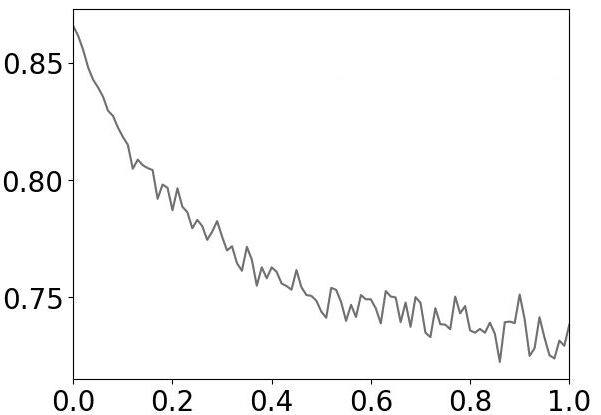
\includegraphics[width=0.48\textwidth]{media/From_IEEE/res_elec_100_h_10_rerun.csv_F1_score_reduced.jpg}
         \label{fig:f1_elec}}
    \subfloat[]{
         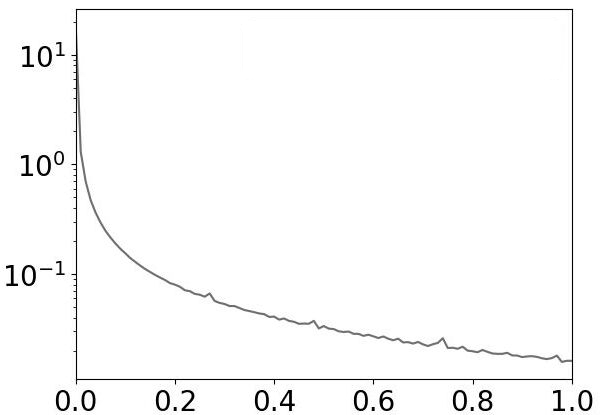
\includegraphics[width=0.48\textwidth]{media/From_IEEE/res_elec_100_h_10_rerun.csv_iter_time_reduced.jpg}
         \label{fig:iter_elec}}
    \\
    \subfloat[]{
         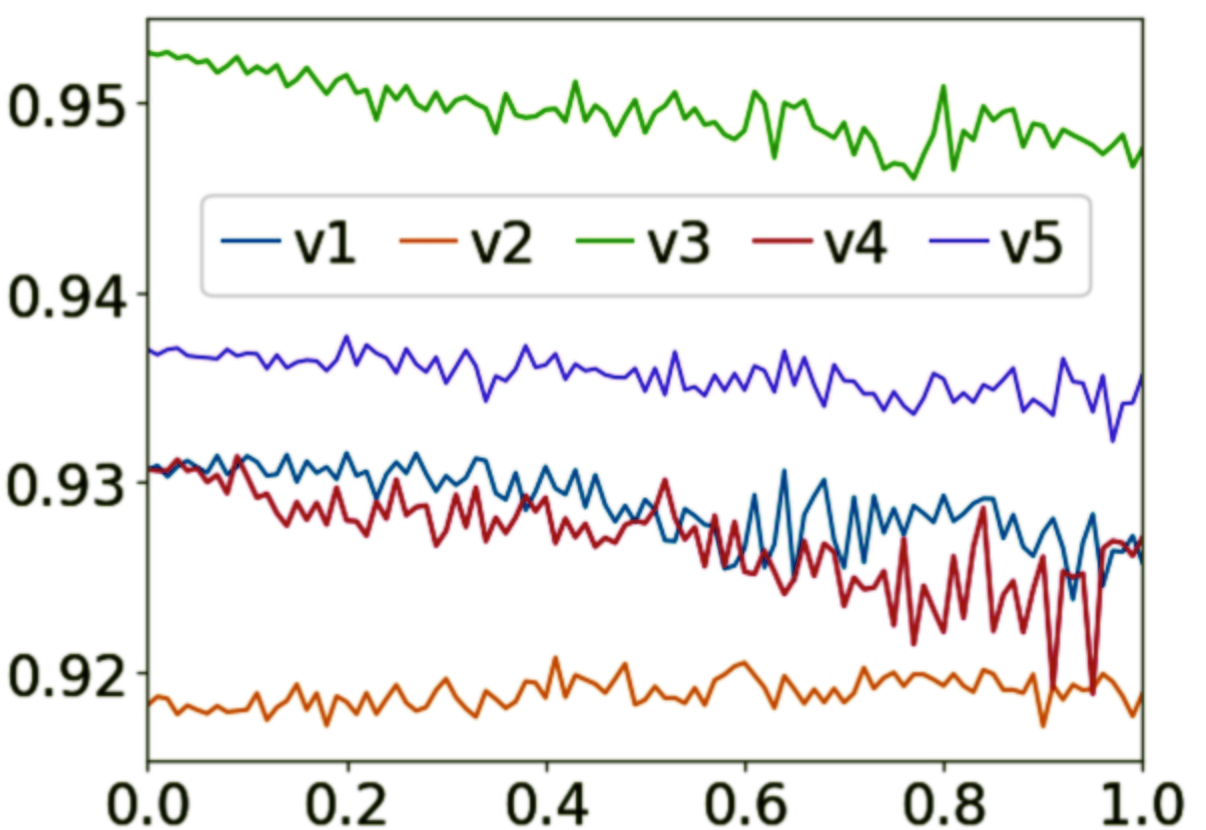
\includegraphics[width=0.48\textwidth]{media/From_IEEE/INSECTS-aggregated_3_F1_score.jpg}
         \label{fig:f1_insects}}
    \subfloat[]{
         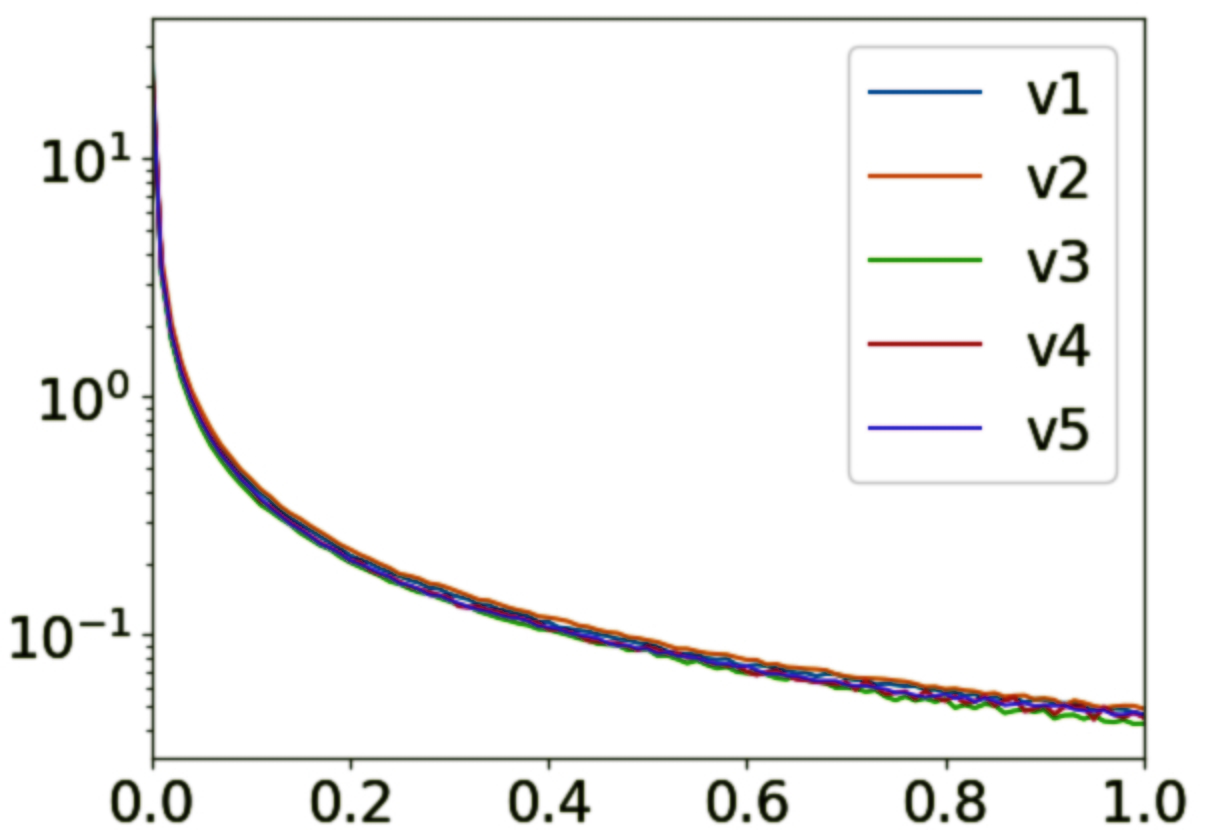
\includegraphics[width=0.48\textwidth]{media/From_IEEE/INSECTS-aggregated_3_iter_time_reduced.jpg}
         \label{fig:iter_insects}}
    \\
    \subfloat[]{
         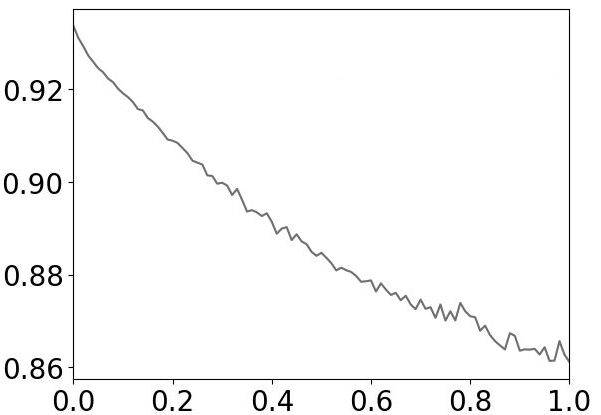
\includegraphics[width=0.48\textwidth]{media/From_IEEE/res_poker-lsn_1000_h_10.csv_F1_score_reduced.jpg}
         \label{fig:f1_poker}}
    \subfloat[]{
         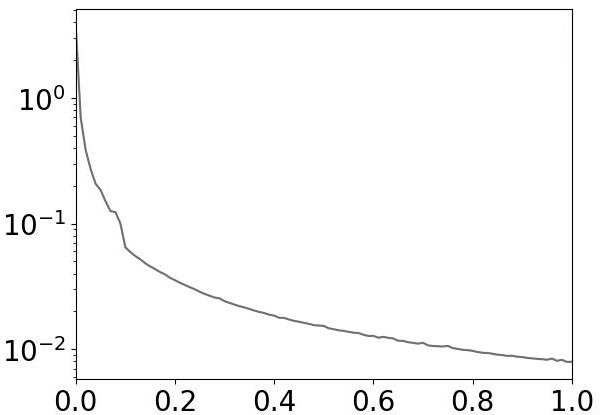
\includegraphics[width=0.48\textwidth]{media/From_IEEE/res_poker-lsn_1000_h_10.csv_iter_time_reduced.jpg}
         \label{fig:iter_poker}}
\caption{Performance of \algo\ in the SW model on the Electricity, INSECTS and Poker datasets (top to bottom), in terms of F1-score (left) and amortized milliseconds per update (right) as a function of $\epsilon$.}\label{fig:SW}
\vspace*{10pt}
\end{figure}

\begin{figure}
\vspace*{10pt}
    \centering
    \subfloat[]{
         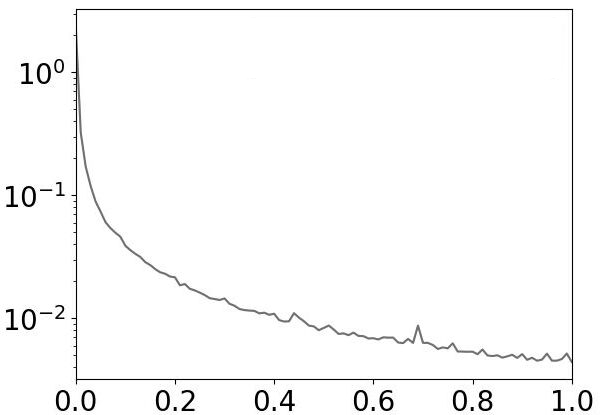
\includegraphics[width=0.5\textwidth]{media/From_IEEE/elec_random.csv_iter_time_reduced.jpg}
         \label{fig:ru_elec}    
    }
    \hfill
    \subfloat[]{
         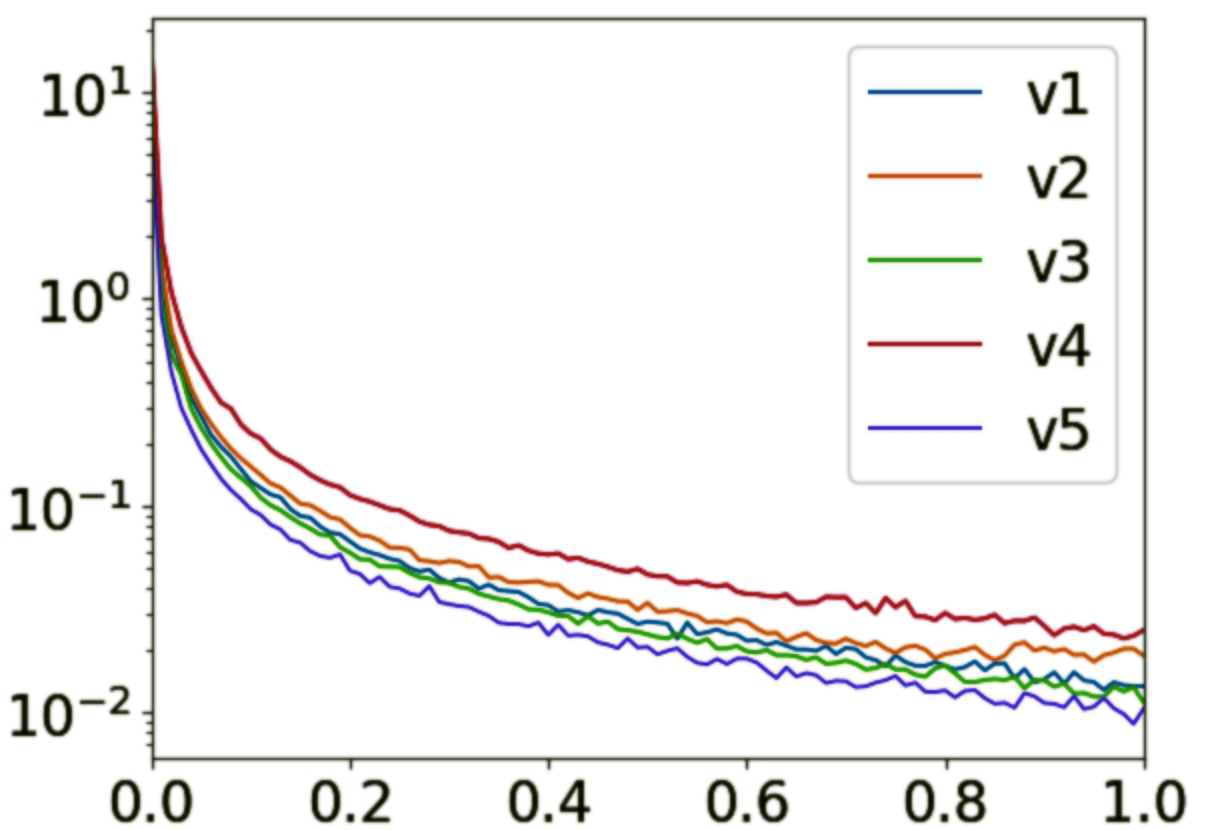
\includegraphics[width=0.5\textwidth]{media/From_IEEE/INSECTS_random-aggregated_3_iter_time_reduced.jpg}
         \label{fig:ru_insects}    
    }
    % \\[15pt]
    % \subfloat[]{
    %      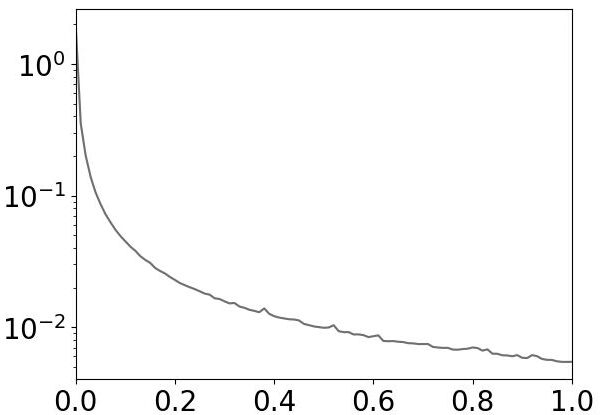
\includegraphics[width=0.5\textwidth]{media/From_IEEE/poker-lsn_random.csv_iter_time_reduced.jpg}
    %      \label{fig:ru_poker}    
    % }
%\caption{Amortized running time of \algo\ in the RU model on the Electricity (left) and INSECTS (right) datasets. Amortized running time for the Poker dataset is very similar to Electricity.}

\caption{Amortized running time per update (in milliseconds) of \algo\ in the RU model on the Electricity (left) and INSECTS (right) datasets. The Poker dataset yields similar results.}

\label{fig:RU}
\end{figure}




\iffalse
\begin{figure*}
    \centering
    \subfloat[Electricity (F1-score)]{
         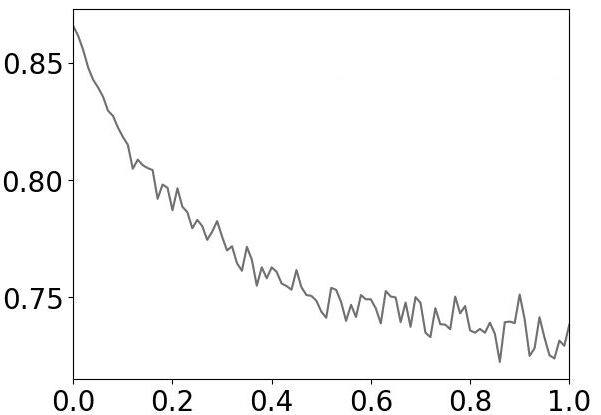
\includegraphics[width=0.3\textwidth]{media/From_IEEE/res_elec_100_h_10_rerun.csv_F1_score_reduced.jpg}
         \label{fig:f1_elec}}
    \hfill
    \subfloat[INSECTS (F1-score)]{
         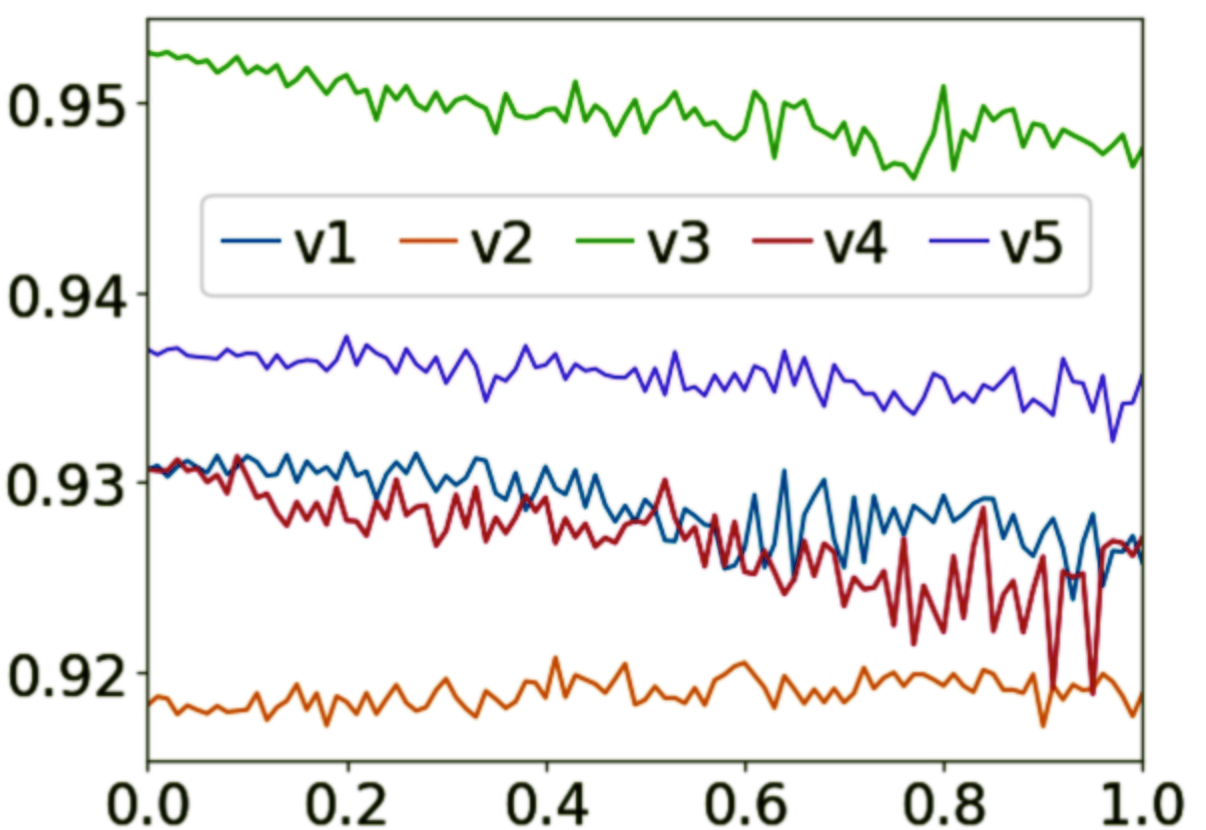
\includegraphics[width=0.28\textwidth]{media/From_IEEE/INSECTS-aggregated_3_F1_score.jpg}
         \label{fig:f1_insects}}
    \hfill
    \subfloat[Poker (F1-score)]{
         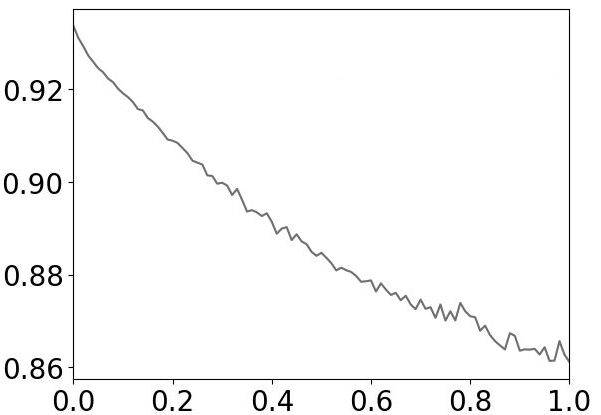
\includegraphics[width=0.3\textwidth]{media/From_IEEE/res_poker-lsn_1000_h_10.csv_F1_score_reduced.jpg}
         \label{fig:f1_poker}    
    }
    \label{fig:f1_scores}
    \subfloat[Electricity (Time)]{
         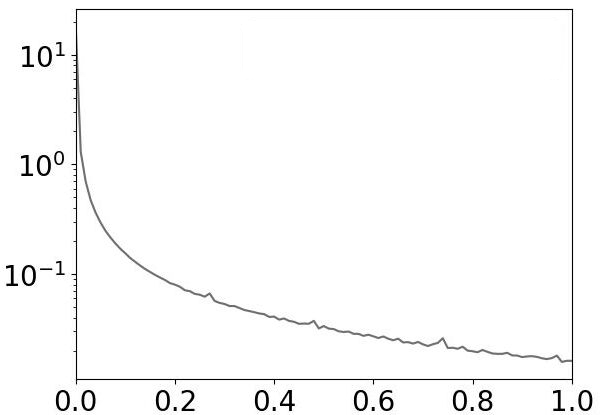
\includegraphics[width=0.3\textwidth]{media/From_IEEE/res_elec_100_h_10_rerun.csv_iter_time_reduced.jpg}
         \label{fig:iter_elec}    
    }
    \hfill
        \subfloat["INSECTS" (Time)]{
         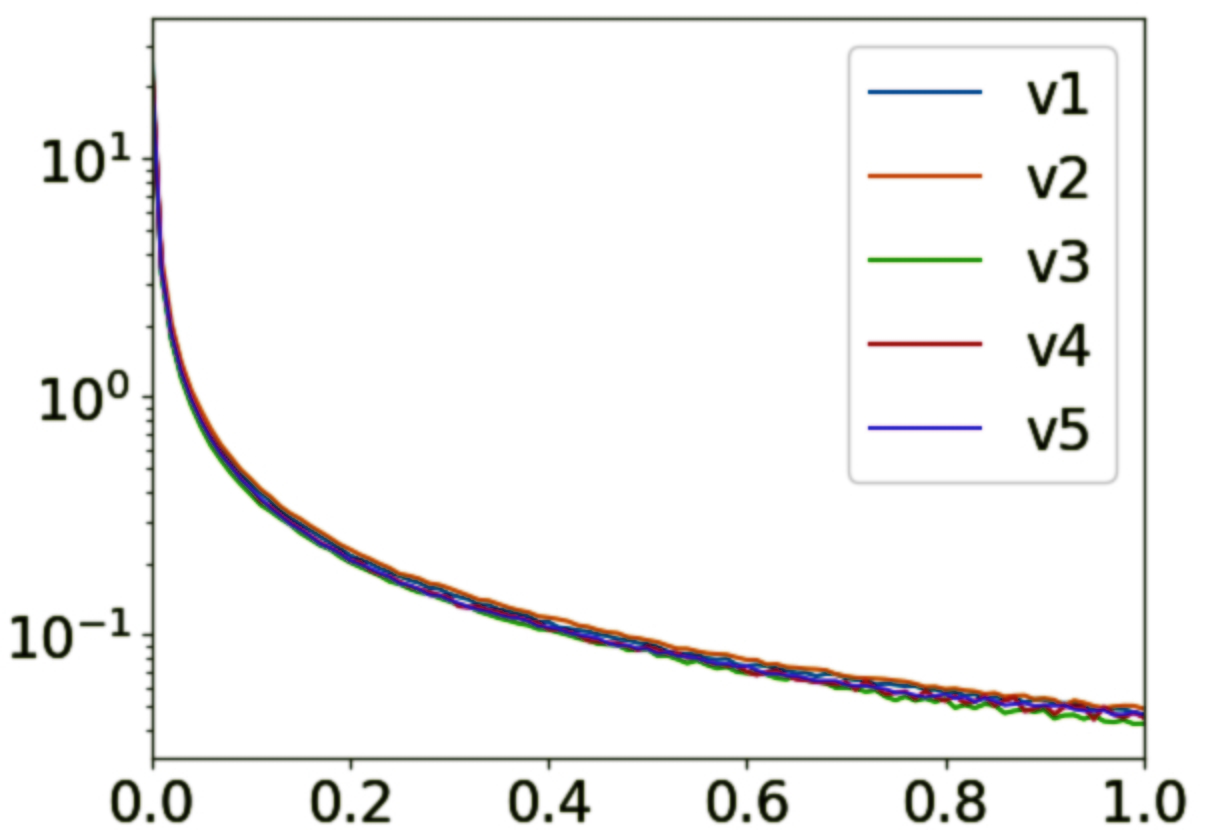
\includegraphics[width=0.28\textwidth]{media/From_IEEE/INSECTS-aggregated_3_iter_time_reduced.jpg}
         \label{fig:iter_insects}    
    }
    \hfill
    \subfloat[Poker (Time)]{
         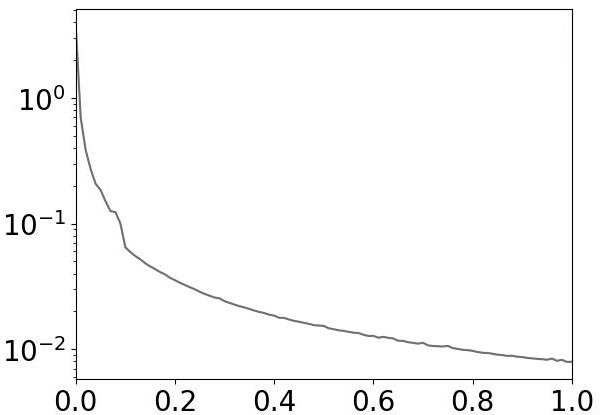
\includegraphics[width=0.3\textwidth]{media/From_IEEE/res_poker-lsn_1000_h_10.csv_iter_time_reduced.jpg}
         \label{fig:iter_poker}    
    }
\caption{F1-score and amortized running time in the SW model.}\label{fig:SW}

\end{figure*}
\fi

\iffalse
\begin{figure*}
    \centering
    \subfloat[Electricity]{
         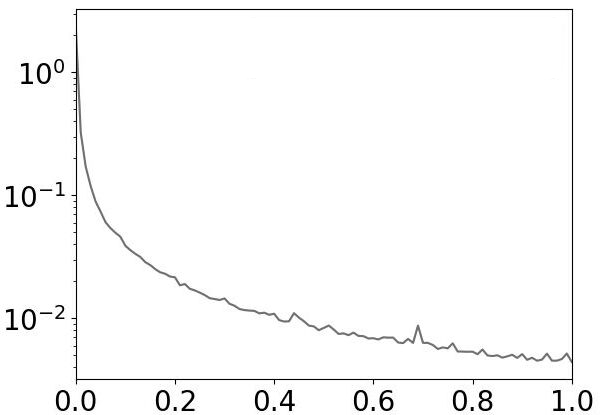
\includegraphics[width=0.3\textwidth]{media/From_IEEE/elec_random.csv_iter_time_reduced.jpg}
         \label{fig:ru_elec}    
    }
    \hfill
    \subfloat[INSECTS]{
         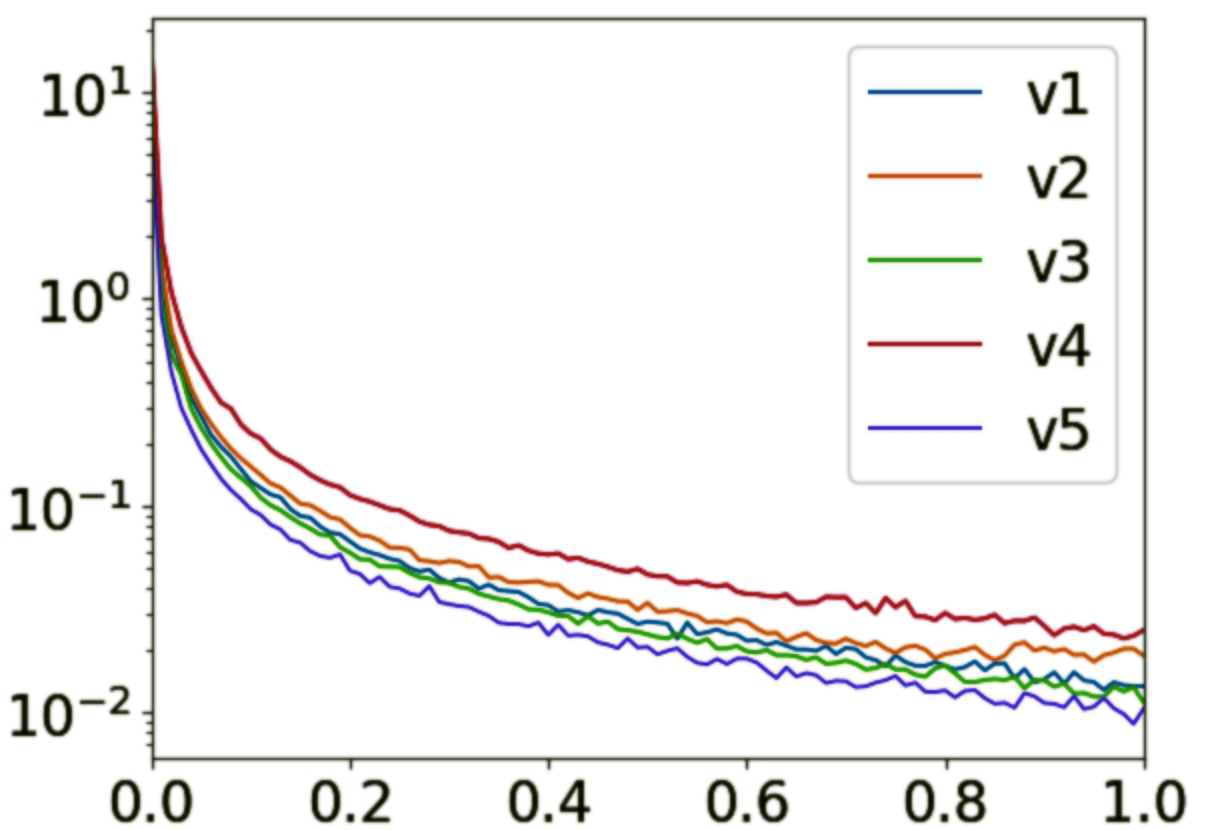
\includegraphics[width=0.28\textwidth]{media/From_IEEE/INSECTS_random-aggregated_3_iter_time_reduced.jpg}
         \label{fig:ru_insects}    
    }
    \hfill
    \subfloat[Poker]{
         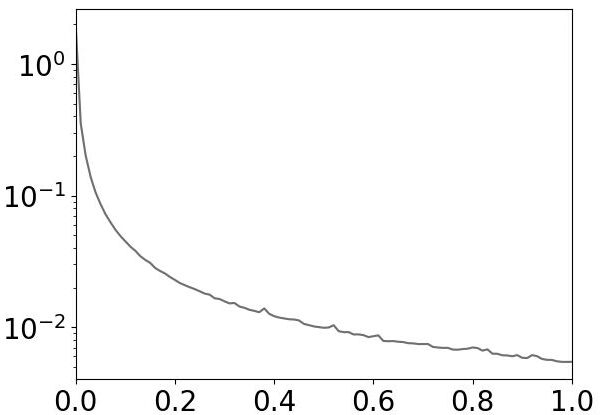
\includegraphics[width=0.3\textwidth]{media/From_IEEE/poker-lsn_random.csv_iter_time_reduced.jpg}
         \label{fig:ru_poker}    
    }
\caption{Amortized running time in the RU model.}\label{fig:RU}
\end{figure*}
\fi

%\iffalse
\subsection{Conclusions and Future Work}
We developed the first fully dynamic algorithm for maintaining $\epsilon$-feasible decision trees, while we proved it to be nearly optimal in terms of space and amortized time. Our work shows that many well-known decision tree algorithms, whether offline like CART or incremental like EDFT, can be made fully dynamic with a small loss in the quality of the decision tree and a small overhead in the amortized running time. Our work leaves open the natural question of whether these results can be strengthened from amortized to worst-case. We believe this is an exciting direction for future research in  fully-dynamic supervised machine learning.
%We developed the first fully dynamic algorithm for maintaining $\epsilon$-feasible decision trees, as well as lower bounds on the space requirements and amortized running time of any such algorithm. Our algorithm boasts near-optimal space requirements and near-optimal running time for some cases of interest. Our experimental evaluation shows that our algorithm is accurate in terms of F1-score, while boasting an average running per update of less than one millisecond. We believe that developing fully-dynamic algorithms for supervised machine learning problems is an exciting research direction that deserves more attention. 
%\fi
\chapter{Personalized PageRank for Graph Embedding}
\section{Introduction}
\subsection{Our contributions}
\subsection{Organization of the chapter}
\section{PageRank}
The PageRank score was briefly introduced in section \ref{subsec:Intro_centrality}. We propose here an in-depth study of this metric and its personalized version, its theoretical properties and its practical computation.

Let's first recall the definition of the PageRank score.

\subsection{Equivalent definitions of PageRank and PPR} \label{subsec:ppr_definitions}
\subsubsection{PageRank}
The first definition of PageRank with a parameter $\alpha \in [0, 1)$ was that of a random walk with restart in the graph. The walker starts from a vertex drawn uniformly at random and at each step, it makes one of the following two moves:
\begin{description}
    \item[Restart] The walker chooses any vertex of the graph at random and jumps to it.
    \item[Walk] The walker draws uniformly at random one of the neighbors (out-neighbors in the case of directed graphs) of the vertex it is on and goes to that neighbor.
\end{description}

At each step, the probability to restart is $\alpha$ and the probability to walk is $1-\alpha$. Let's note $p_i \in \realset^n$ the vector that, for each vertex, contains the probability of being on that vertex at step $i$. The random walk is defined by the following sequence:
\begin{equation}\label{eq:pr_def_as_sequence}
    \begin{cases}
        p_0 = \frac{1}{n}\ones\\
        p_{i+1}^\top = \alpha \underbrace{p_0^\top}_{\text{Restart}} + (1-\alpha)\underbrace{p_i^\top M}_{\text{Walk}}
    \end{cases}
\end{equation}
where $\ones \in \realset^n$ is the vector of which all elements are $1$.

\begin{property}\label{prop:pr_def_as_equation}
    The sequence defined in equation \ref{eq:pr_def_as_sequence} converges to the vertex $\pi$ defined by 
    \begin{equation}\label{eq:pr_def_as_equation}
        \pi^\top = \alpha p_0^\top + (1-\alpha)\pi^\top M
    \end{equation}
\end{property}
\begin{proof}
    Let $f : \realset^n \rightarrow \realset^n$ be the iteration function, $f(x)^\top =\alpha p_0^\top + (1-\alpha)p_i^\top M$. We have 
    \begin{equation*}
        \forall x, y \in \realset^n : f(x)^\top - f(y)^\top = (1-\alpha)(x-y)^\top M
    \end{equation*}
    Since $M$ is a stochastic matrix, we have $\forall z \in \realset^n : ||z^\top M||_1 \leq ||z||_1$. Therefore, we have 
    \begin{equation*}
        \forall x, y \in \realset^n : ||f(x)^\top - f(y)^\top||_1 \leq (1-\alpha)||(x-y)||_1
    \end{equation*}
    This proves that $f$ is a contraction mapping on $\realset^n$ and so the Banach fixed-point theorem concludes the proof.
\end{proof}

The PageRank vector of the graph $G$ is the asymptotic limit of the sequence defined in equation \ref{eq:pr_def_as_sequence}, i.e. it is the vector $\pi$ defined in equation \ref{eq:pr_def_as_equation}.

\begin{property}\label{prop:pr_def_as_series}
    The PageRank vector $\pi$ defined in equation \ref{eq:pr_def_as_equation} can be equivalently written as the series
    \begin{equation}\label{eq:pr_def_as_series}
        \pi^\top = \alpha \sum_{i = 0}^{+\infty} (1-\alpha)^i p_0^\top M^i
    \end{equation}
\end{property}
\begin{proof}
    We can show by induction that the general term of the sequence described in equation \ref{eq:pr_def_as_sequence} is
    \begin{equation*}
        p_i = (1-\alpha)^i p_0^\top M^i + \alpha \sum_{j = 0}^{i-1} (1-\alpha)^j p_0^\top M^j
    \end{equation*}

    It has already been shown that the sequence converges. 
    
    Given that $\lim_{i \to +\infty} ||(1-\alpha)^i p_0^\top M^i||_1 = 0$ then
    \begin{equation*}
        p_i \sim_{i \to +\infty} \alpha \sum_{i = 0}^{i-1} (1-\alpha)^i p_0^\top M^i
    \end{equation*}
\end{proof}

\subsubsection{Personalized PageRank}
In a graph $G = \{V, E\}$, the Personalized PageRank (PPR) vector $\pi_u$ of a vertex $u \in V$ with parameter $\alpha$ is the asymptotic vector of the sequence defined by 
\begin{equation}\label{eq:ppr_def_as_sequence}
    \begin{cases}
        p_0 = e_u\\
        p_{i+1}^\top = \alpha p_0^\top + (1-\alpha)p_i^\top M
    \end{cases}
\end{equation}
with $e_u \in \realset^n$ the vector of which the only non-zero element is $1$ at the $u$\textsuperscript{th} position.

This definition is identical to equation \ref{eq:pr_def_as_sequence} except for the first term. It is easy to see that properties \ref{prop:pr_def_as_equation} and \ref{prop:pr_def_as_series} also apply.

\begin{definition}[Personalized PageRank (PPR) matrix]
    The \define{Personalized PageRank matrix} $\Pi \in \realset^{n \times n}$ of a graph $G = \{V, E\}$ with parameter $\alpha$ is the matrix of which each line is the PPR vector of the related vector of the graph.
\end{definition}

We know from properties \ref{prop:pr_def_as_equation} and \ref{prop:pr_def_as_series} that
\begin{equation*}
    \pi_u^\top = \alpha e_u^\top + (1-\alpha) p_u^\top M
\end{equation*}
and
\begin{equation*}
    \pi_u^\top = \alpha \sum_{i=0}^{+\infty} (1-\alpha)^i e_u^\top M^i
\end{equation*}

We can deduce that
\begin{equation}\label{eq:ppr_mat_as_equation}
    \Pi = \alpha I + (1-\alpha)\Pi M
\end{equation}
and
\begin{equation}\label{eq:ppr_mat_as_series}
    \Pi = \alpha \sum_{i=0}^{+\infty} (1-\alpha)^i M^i
\end{equation}
where $I\in \realset^{n\times n}$ is the identity matrix.

Finally, we see from equation \ref{eq:ppr_mat_as_equation} that 
\begin{equation} \label{eq:ppr_mat_as_inverse}
    \Pi = \alpha (I - (1-\alpha)M)^{-1}
\end{equation}

Note that $I - (1-\alpha)M$ is a strictly diagonally dominant matrix, and hence is invertible.

\subsubsection{Interpretations}
A first interpretation of the PageRank and Personalized PageRank vectors has been given in its definition. We propose two other interpretations.

In the first new interpretation, a content (e.g. information, liquid\dots) flows from the vertices in $p_0$. At each step, a fraction $\alpha$ of the still-flowing content it kept or dissipated on its current vertex and the rest divides equally to keep flowing to the neighbors. The PageRank or PPR vector is the proportion of the content that have been kept or dissipated on each vertex, i.e. the exposure of each vertex to the content.

The second interpretation comes directly from equation \ref{eq:ppr_mat_as_series} and uses another random walk. In this new random walk, the initial position of the walker is selected as in the definition of PageRank or PPR, but then the actions of the walker are one of these two:
\begin{description}
    \item[Stop] The walker stops walking and the random walk ends
    \item[Walk] The walker draws uniformly at random one of the neighbors (out-neighbors in the case of directed graphs) of the vertex it is on and goes to that neighbor.
\end{description}

The probability of stopping is $\alpha$. The value for a vertex $v$ in the PageRank or PPR vector is the probability that the walker is on that vertex when he stops walking. This interpretation helps to understand why it is usually enough to compute only a few steps of the walk to approximate the PageRank or PPR vectors. For example, if $\alpha = 0.1$ then after only $66$ steps the probability that the walker is still walking is less than $10^{-3}$.

\subsection{Properties of the PPR matrix}
\begin{theorem} The multiplication of $\Pi$ with $M$ is symmetrical
    \[\Pi M = M \Pi\]
\end{theorem}
\begin{proof}
    \begin{equation*}
    \begin{split}
        \Pi M - M \Pi & = \cancel{\alpha M} + (1-\alpha)\Pi M^2 \cancel{- \alpha M} - (1-\alpha) M \Pi M\\
        & = (1-\alpha)(\Pi M - M \Pi) M
    \end{split}
\end{equation*}
so $$(\Pi M - M \Pi)(I - (1-\alpha)M) = 0_{\mathbb{R}^{n \times n}}$$ with $0_{\mathbb{R}^{n \times n}} \in \mathbb{R}^{n \times n}$ the zero matrix.

Since $(I - (1-\alpha)M)$ is invertible, we deduce that
\[(\Pi M - M \Pi) = 0_{\mathbb{R}^{n \times n}}\]
\end{proof}

\begin{theorem}
    If the graph $G$ is undirected, then the matrices $D\Pi$ and $\Pi D^{-1}$ are symmetrical.\todo{Mention now or later that it would allow eigendecomposition, but not studied yet}
\end{theorem}
\begin{proof}
     We first prove that $\Pi D^{-1}$ is symmetrical. We note that since $G$ is undirected, $A$ is symmetrical. We also recall that $\forall A, B$ invertible matrices, $(AB)^{-1} = B^{-1} A^{-1}$.
     
     We use the definition of $\Pi$ given by the equation \ref{eq:ppr_mat_as_inverse}. Then we have 
    \begin{equation*}
        \begin{split}
            \Pi D^{-1} &= \alpha (I - (1-\alpha) M)^{-1} D^{-1}\\
            &= \alpha (D - (1-\alpha) D \underbrace{M}_{= D^{-1} A})^{-1}\\
            &= \alpha (D - (1-\alpha) D \underbrace{A D^{-1} D}_{=M^\top D})^{-1}\\ 
            &= \alpha D^{-1}(I - (1-\alpha) M^\top)^{-1}\\
            &= D^{-1}\Pi^\top
        \end{split}
    \end{equation*}
    The proof that $D\Pi$ is symmetric follows directly from $\Pi D^{-1} = D^{-1} \Pi^\top$
\end{proof}

\begin{theorem}\label{th:dpi_pidm_symdefpos}
    If the graph $G$ is undirected, then the matrices $D\Pi$ and $\Pi D^{-1}$ are positive-definite
\end{theorem}
We note that if a matrix $\Gamma$ is symmetric and positive-definite, then there is an eigendecomposition $\Gamma = U D U^\top$ so that $U$ is a unitary matrix and $D$ is diagonal and strictly positive. Therefore, the inverse matrix $\Gamma^{-1} = U D^{-1} U^\top$ is also symmetric and positive-definite. We also know from equation \ref{eq:ppr_mat_as_inverse} that the inverse of $D\Pi$ and $\Pi D^{-1}$ are respectively $\frac{1}{\alpha} \big(D^{-1} - (1-\alpha)D^{-1} A D^{-1}\big)$ and $\frac{1}{\alpha} \big(D - (1-\alpha)A\big)$. The proof will therefore consist in proving that the matrices $\big(D^{-1} - (1-\alpha)D^{-1} A D^{-1}\big)$ and $\big(D - (1-\alpha)A\big)$ are positive-definite, i.e. that the quadratic forms defined by these matrices over $\realset^n$ is an inner product.

\begin{proof}[Proof that $\big(D^{-1} - (1-\alpha)D^{-1} A D^{-1}\big)$ is positive-definite]

    $\forall x \in \realset^n$, we have
    \begin{equation*}
        \begin{split}
            x^\top \big(D^{-1} - (1-\alpha)D^{-1} A D^{-1}\big) x &= \sum_{u=1}^n \frac{x_u^2}{d_u} - (1-\alpha)\sum_{u=1}^n \sum_{v=1}^n \frac{x_u x_v}{d_u d_v} a_{uv}\\
            & = \alpha \sum_{u=1}^n \frac{x_u^2}{d_u} + (1-\alpha)\sum_{u=1}^n\big(\frac{x_u^2}{d_u} - \sum_{v=1}^n \frac{x_u x_v}{d_u d_v} a_{uv}\big)\\
            & = \alpha \sum_{u=1}^n \frac{x_u^2}{d_u} + (1-\alpha)\sum_{u=1}^n\sum_{v=1}^n\frac{x_u}{d_u}\big(\frac{x_u}{d_u} - \frac{x_v}{d_v}\big)a_{uv}\\
            & = \alpha \sum_{u=1}^n \frac{x_u^2}{d_u} + \frac{1-\alpha}{2}\sum_{u=1}^n\sum_{v=1}^n\big(\frac{x_u}{d_u} - \frac{x_v}{d_v}\big)^2a_{uv}\\
        \end{split}
    \end{equation*}
    We see that $x^\top \big(D^{-1} - (1-\alpha)D^{-1} A D^{-1}\big) x \geq 0$ and that $0$ is reached only when $x=\zeros{\realset^n}$
\end{proof}

\begin{proof}[Proof that $\big(D - (1-\alpha) A\big)$ is positive-definite]

With a similar reasoning as for $\allowbreak\big(D^{-1} - (1-\alpha)D^{-1} A D^{-1}\big)$, we get that $\forall x \in \realset^n$, we have
\begin{equation*}
    x^\top\big(D - (1-\alpha) A\big)x = \alpha \sum_{u=1}^n d_u x_u^2 + \frac{1-\alpha}{2}\sum_{u=1}^n\sum_{v=1}^n(x_u - x_v)^2a_{uv}\\ 
\end{equation*}
\end{proof}

\subsection{Computing the PPR matrix and vectors}
We note $\pi(p_0)$ the PPR vector generated from the PageRank random walk with restart using $p_0$ as the initial vector. This can be the PageRank vector, a rooted PPR vector, or any PPR vector starting from a set of nodes.

The main idea of this algorithm is to build sequences $(q_i)_{i\in \naturalset}$ and $(r_i)_{i\in \naturalset}$ that maintain the following invariant
\begin{equation}\label{eq:ppr_alg_invariant}
    \forall i \in \naturalset, \big(\pi(p_0)\big)^\top = q_i^\top + r_i^\top\Pi
\end{equation}

The pseudocode is shown as Algorithm \ref{alg:ppr_invariant}. In this algorithm, the vectors $p_i$ are the successive approximations of the PPR vector, while the vectors $r_i$ are the residual values that are still to be considered in the approximation. This algorithm can be seen as a simulation of the interpretation as content flowing given in section \ref{subsec:ppr_definitions}. With that interpretation, $p_i$ is the content that has already stopped while $r_i$ represents the content that keeps flowing.

The convergence of this algorithm is guaranteed by the fact that $M$ is a stochastic matrix and hence $\forall i \in \naturalset : ||r_iM||_1 \leq ||r_i||_1$. Therefore $\forall i \in \naturalset : ||r_{i+1}||_1 \leq (1-\alpha)||r_i||_1$. $||r_i||_1$ is upper bounded by a geometric sequence of common ratio less than 1, therefore it converges to $\zeros{\realset^n}$ and, thanks to the invariant in equation \ref{eq:ppr_alg_invariant}, we deduce that $q_i$ converges to $\pi(p_0)$

\begin{algorithm}
\caption{PPR computing algorithm using an invariant}
\label{alg:ppr_invariant}
\begin{algorithmic}[1]
    \Require $\alpha$ the parameter of the PPR walk, $M$ the stochastic matrix of a random walk in the graph, $q_0 \in (\realset^+)^n : ||q_0||_1 = 1$ the initial random walk vector, $max\_iter\in \naturalset$ the number of iterations and/or $\varepsilon \in (0, 1)$ the maximum accepted residual value.

    \State $i = 0$
    \State $q_i = \zeros{\realset^n}$
    \State $r_i = q_0$

    \While{$i<max\_iter$ and $||r_i||_1 < \varepsilon$}
        \State $i++$
        \State $p_i = p_{i-1} + \alpha r_{i-1}$
        \State $r_i^\top = (1-\alpha) r_{i - 1}^\top M$
    \EndWhile
    \State \Return $p_i$
\end{algorithmic}
\end{algorithm}\todo{Check if true name exists}

\section{Graph Embedding and Matrix Factorization}
\subsection{Taxonomy of graph embedding methods}
As introduced in section \ref{subsec:intro_graph_embedding}, the objective of graph embedding is to find a function $\phi: V \rightarrow \realset^k$ that represents the vertices of the studied graph into a low-dimension vectorial space $\realset^k$. The function can be represented as a matrix $Y \in \realset^{n\times k}$ in which each line is the embedding of the related vertex. There exists in the literature a consensual taxonomy of the methods to perform such embedding \cite{cai2018_ComprehensiveSurveyGraph, goyal2018_GraphEmbeddingTechniques}. This taxonomy contains three main classes of techniques, namely the Matrix Factorization, the Random Walk and the Deep Learning techniques.

A Matrix Factorization technique is based on a $n \times n$ matrix $X$ of which each element represents some sense of proximity between the two related vertices. For example, the simplest of these matrices is the adjacency matrix $A$ of the graph. Then a factorization method as the eigendecomposition or the Singular Value Decomposition is used and parts or all of the results of this decomposition are used as the embedding results. When a non-symmetrical decomposition is performed as the SVD $X \approx U \Sigma V^\top$, each vertex can receive an embedding both from $U$ and $V$. In that case, the embeddings from $U$ and $V$ are usually called respectively \define{left embedding} and \define{right embedding}.

A Random Walk technique consists in sampling random walks in the graph and then embed these random walks, considering that they reflect the structure of the graph.

Some Matrix Factorization techniques are deeply related to Random Walk techniques because the matrices they are based on represent probabilities to go from one edge to another in a random walk. For example, as defined in section \ref{subsec:ppr_definitions}, the Personalized PageRank matrix is the probability matrix of a random walk with restart and therefore the matrix and an embedding derived from it could be approximated by sampling this random walk.

Finally, as suggested by their name, Deep Learning techniques rely on deep learning algorithms to learn the embedding of the vertices. Two main approaches exist, namely Autoencoder techniques and Graph Convolutional Networks (GCN). Autoencoders are Neural Networks that consist in a first part called the \define{encoder} of which role is to compute the embedding and a second part called the \define{decoder} of which role is to retrieve the graph or part of it based on the embedding vectors. The two parts are trained together in an unsupervised manner. Graph Convolutional Networks on the other first find an embedding based on the direct neighborhood of each vertex, and then iteratively takes into account the embedding of vertices further away.

\subsection{A brief history}\label{subsec:embedding_history}
One of the first graph embedding techniques was introduced in 2001 and is called \define{spectral embedding} \cite{belkin2001_spectralEmbedding}. Given an undirected graph, its Laplacian matrix $ L = D - A$ is symmetric and positive semidefinite. Therefore, this matrix has an eigendecomposition, i.e. there exist a diagonal matrix $D \in \realset^{n\times n}$ and an unitary matrix $U \in \realset^{n \times n}$ so that:
\begin{equation}
    A = U D U^\top
\end{equation}

The values in $D$ called \define{eigenvalues} are in increasing order. The first eigenvalue will always be $0$, and there will be as many eigenvalues that are $0$ as there are connected components in the matrix \cite{belkin2001_spectralEmbedding}. The embedding vectors, are the columns of $U$, called \define{eigenvectors}, except for the first one which corresponds to the eigenvalue of 0.

If we note $Y$ the embedding matrix, this embedding has been shown by \cite{belkin2001_spectralEmbedding} to solve the following problem:
\begin{equation}
    Y = \begin{cases}
    \begin{aligned}
        \min_{X \in \realset^n} &\sum_{u = 1}^n\sum_{v=1}^n ||X_u - X_v||_2^2a_{uv}\\
        \text{s.t.  } & X^\top \ones = \zeros{\realset^k}\\
                    & X^\top X = I
    \end{aligned}
    \end{cases}
\end{equation}

The first constraint $X^\top \ones = \zeros{\realset^k}$ ensures that the embeddings are centered, and the second constraint $X^\top X = I$ ensures that the embedding dimensions are uncorrelated.\todo{Add note about relation with PPR spectral embedding}

In 2014 was presented the first Random Walk embedding named DeepWalk \cite{perozzi2014_DeepWalkOnlineLearning}. This algorithm consists in sampling random walks of fixed length and it considers the sequence of vertices that form each random walk as a sentence of a corpus. The embedding is then computed by using Language Processing tools. Specifically, this method uses the SkipGram words embedding model.

This idea was taken one step further in 2016 with the very famous embedding method called node2vec \cite{groverNode2vecScalableFeature2016}. In this method, the random walk is biased by two parameters $p$ and $q$. The parameter $p$ limits the “return” likelihood of the random walk, i.e. a high value of $p$ will make it unlikely that the walker goes back to the node it just left. The parameter $q$ limits the “spreading” behavior of the random walk, i.e. a high value of $q$ will make it unlikely that the walker goes to a neighbor of the current node that would not also be a neighbor of the previous node.



\subsection{The problem of interpretability}\label{subsec:interpretability_explained}
%Note: Copied directly from the paper
The interest for explainable algorithms is growing recently among the broad research community and in the general public alike. Many data-processing algorithms are fed with embeddings of complex data. If the embedding methods are not interpretable, there is little hope to provide satisfying explanations of the result of the algorithm. As a result, many recent papers focus on developing embedding methods that are interpretable, such as~\cite{example_interpr_lee_2021} and~\cite{example_interpr_wu_2020}, for image and video processing, respectively.
In the field of graph embeddings, most of the efforts have focused on defining measures to assess the interpretability of a graph embedding algorithm, with community-based metrics emerging as one of the most popular metrics. In particular, \cite{khoshraftar2021} and \cite{gogoglou_2019} develop three different community-based interpretability metrics and evaluate node2vec and HOPE in terms of those metrics. Those works suggest that a satisfactory solution for an interpretable graph embedding is still missing. %Our work aims at filling this gap, focusing on developing an effective and interpretable graph embedding. 

\subsubsection{Metrics overview}\label{sec:metrics}
Several metrics have been proposed to evaluate the interpretability of a graph embedding, such as the Interpretability Score (IS)~\cite{gogoglou_2019}, the Betweenness Centrality Importance (BCI) and Closeness Centrality Importance (CCI)~\cite{khoshraftar2021}. Those metrics all consider the vector representation of a given node interpretable if it encodes somehow whether that node belongs to some real-world communities. 

%We evaluate the results of our algorithms in terms of IS.  We also study the BCI and CCI, however, due to the strong limitations of BCI and CCI, discussed in Section~\ref{subsec:bci_cci_introduction} and because of space limitations, we do not include them in our experimental evaluation. Finally, we propose the new Complete Interpretability Score Integrating Priority (CISIP) metric to tackle some weaknesses of the previous metrics.
\todo{Check that we explain somewhere which metrics we use and why}
% and Closeness Centrality Importance (CCI) presented by \cite{khoshraftar2021} but, due the strong limitations of these metrics discussed in section \ref{subsec:bci_cci_introduction} and because of space limitations, we do not include them in our experiments. Finally, we propose the new Complete Interpretability Score Integrating Priority (CISIP) metric to tackle some weaknesses of the existing ones.


\subsubsection{Interpretability score (IS)}
Let $k$ be the index of one of the embedding dimensions, and $C_g$ one of the ground-truth communities. The IS for a $(k, g)$ pair is decomposed into a top part $IS_{top(k, g)}$ 
%that equals the proportion of the $|C_g|$ vertices of maximum score in the embedding that belong to $C_g$,
that equals the recall@$|C_g|$ of the top-scores vertices of the embedding, i.e. the $|C_g|$ vertices of maximum score in the embedding that belongs to $C_g$, and a bottom $IS_{bottom(k, g)}$ part defined similarly on the lowest scores.
These parts evaluate respectively how well the highest and lowest scores of the embedding reflect the belonging to the group.

The article then proposes to aggregate the scores by dimension or ground-truth group using either average or maximum function.\todo{The technical details of how we use it should be described in the "Experiments" part (maybe with the equation commented below)} %In this paper we will use the maximum. It is also suggested in \cite{gogoglou_2019} that the scores should be aggregated either by embedding dimension or by ground-truth group.
%In order for us to obtain a single result score for the entire embedding, we will aggregate first by taking the maximum IS per embedding dimension over the ground-truth groups and then the mean over all embedding dimensions.
%The use of the mean allows us to obtain scores between 0 and 1. % but we should keep in mind that, counterintuitively, it makes it possible that the adding of new dimensions to the embedding worsens it score.
%In contrast with \cite{gogoglou_2019}, we do not multiply the result by 100, which only changes the results by this factor without any other impact.

\begin{equation}
    IS = \sum_{k=1}^K \text{agg}_{g \in [0, G]}\big(\text{agg}(IS_{top(k,g)}, IS_{bottom(k,g)})\big)
\end{equation}
% \begin{equation}
%     IS = \frac{1}{K}\sum_{k=1}^K \max_{g \in [0, G]}(\max(IS_{top(k,g)}, IS_{bottom(k,g)})
% \end{equation}

\subsubsection{Betweenness Centrality Importance (BCI) and Closeness Centrality Importance (CCI)}\label{subsec:bci_cci_introduction}
These scores are defined based on the well-known Betweenness Centrality and Closeness Centrality scores, introduced in \cite{bloch2023centrality}. \todo{Maybe introduce it in the "centrality" part} As for the IS, the BCI and CCI scores are split into a top and a bottom part that evaluate respectively how well the top and the bottom nodes of an embedding dimension match a ground-truth group.

For a $(k, g)$ pair, the top BCI score is defined as the normalized Betweenness Centrality in relation with the community, of the top nodes of the dimension that belongs to the community. The CCI top score is defined similarly but using the Closeness Centrality instead of the Betweenness Centrality.\todo{Detail further}
However, the normalization of these scores make them harder to use and interpret. For a $(k, g)$ pair, the scores are normalized by the number of nodes with non-null contribution. Let's consider a community $C_g$ and two embedding dimensions $k_1$ and $k_2$ so that the first one contains only one very central vertex among its top vertices, and the second one contains this same vertex plus another slightly less central vertex. Then, although arguably much more interpretable wrt. the $g$\textsuperscript{th} ground-truth community, the $k_2$ embedding dimension will have a lower score than the $k_1$ one.

\subsubsection{A new interpretability metric: CISIP}

A weak point of the metrics already proposed in the literature is that, although they evaluate the fitness of an embedding dimension to a ground-truth group, they don't evaluate how well the embedding separates the data and the redundancy between the dimensions. Let's take the IS as an example: if 50\% of the $|C_1|$ highest scores for the first dimension belong to $C_1$, then $IS_{top(1,1)} = 0.5$. But then it is possible that 50\% of the highest scores for the second dimension is made either of the exact same part of $C_1$, denoting strong redundancy for the interpretations of these dimensions, or of the other points of $C_1$, denoting that the first group is halved between these dimensions hence reducing the interpretability of both dimensions. In both cases, $IS_{top(2, 1)} = 0.5$.

On top of that all these metrics only consider the nodes that receive top- or bottom-$|C_g|$ scores from the embedding, and all these vertices are considered with equal weight. It seems however natural to consider that the importance should be decreasing before reaching the $|C_g|$ threshold, e.g. the vertex with the highest score should have higher importance than the vertex with the second-highest score.\todo{Illustrate} Similarly, it seems that the importance should not drop to 0 after the $|C_g|$\textsuperscript{th} score: if two embedding dimensions have the exact same top-$|C_g|$ vertices, but one has its $(|C_g|+1)$\textsuperscript{th} vertex belonging to $C_g$ while the other has not, it seems natural to consider that the first one is more interpretable wrt. $C_g$. 

To tackle these weaknesses, we propose the new Complete Interpretability Score Integrating Priority (CISIP) measure. First, we use a function $f$ to smooth the binary belonging feature, providing a score of belonging or importance of each node in each community. The simplest of these functions is simply to use the belonging feature (identity function), but we can also use the Mean Belonging of the Neighbors, the PPR of the community or other functions.

A score is then attributed to each $(k, g)$ pair. Using the Hungarian algorithm for optimal assignment, an exclusive mapping $S = \{(k_i, g_i), i \in [1, \min(K, G)]\}$ of the embedding dimensions to the ground-truth groups is performed. To achieve good performances, the scoring at this step for a couple $(k, g)$ is computed by summing the embedding scores for the dimension $k$ of the vertices that belong to $C_g$. To account for the possibility that the bottom part of the embedding is the part that matches the community, we score in the same way the opposite of the dimension and we take the maximum score of the two. If the score with the opposite is the max, we will then use the opposite of the dimension for the Weighted Kendall Tau scoring.

Then, for each pair $(k_i, g_i) \in S$, a score is computed using Vigna's weighted Kendall Tau score $WKT$ \cite{vigna_2015}. This method provides a score between 0 and 1 of how much the two vectors (embedding score and smoothed ground-truth belonging) are ranked in the same way, with more importance given to the top-scores of each vector. Finally, our metric $CISIP$ is computed as the mean score over the dimensions and groups:
\begin{equation}
    CISIP = \frac{1}{\min(K, G)}\sum_{i=1}^{\min(K, G)}WKT(v_d, f(w_g))
\end{equation}

One weakness of our method that should be noted is that ties in any of the vectors that would not be in the other vector would reduce the score. This behavior is actually wanted when the tie is in the embedding dimension because an embedding with ties that are not in the ground-truth scoring is arguably less interpretable, but it limits drastically the max achievable score when the ground-truth scoring contains many ties (e.g. when the smoothing uses the identity or the Mean Neighbors Belonging function).

\section{A new interpretable graph embedding}%\parfaite{}: PageRank-Matrix Factorization for Interpretable Graph Embeddings}

In a paper presented in the ASONAM conference in 2024\todo{To the best of my knowledge, the proceedings are not available yet. I am not really sure how I should cite this}, we presented a new embedding that we called PAgeRank FActorization-based InTerpretable graph Embedding (\parfaite{}) and that aims first and foremost at providing an highly interpretable graph embedding.

This novel approach is based on the SVD of the PPR matrix. We show in the experimental evaluation presented in section \ref{sec:parfaite_exp} that our method provides higher interpretability scores, while boasting similar results in link prediction than both node2vec and HOPE. To improve the interpretability of our method, we depart from the related work in a number of ways. The main idea of our work is to consider both the PPR matrix and its transposed matrix not only as graph matrices to factorize, but as data matrices that can be processed and mined as such. In particular, in contrast with previous works, our method focuses on the \textit{centered} PPR matrix. This idea comes directly from this vision of the PPR matrix as a data matrix as it is common to center data before mining them. It seems natural to center the PPR matrix, in that, the uncentered matrix is positive, and therefore its first singular vectors are also positive. Moreover, an embedding based on such a positive matrix would use only half of the available space. Observe that centering is also performed in principal component analysis (PCA). As we show in Section~\ref{subsec:interpretation}, centering helps us both reducing biases in the PPR matrix and to interpret the left part of the decomposition of the SVD. We also depart from the related work in the way our embedding is derived from the singular values of the SVD. In particular, virtually all methods based on the SVD of the PPR matrix, use the square root of the singular values to build the vertex embeddings $\mat{U}\mat{\Sigma}^{1/2}$ and $\mat{V}\mat{\Sigma}^{1/2}$. However, when considering the PPR matrix as a data matrix we see that $\mat{U}\mat{\Sigma}$ and $\mat{V}\mat{\Sigma}$ contain some relevant information because they represent the lines and columns of the original matrix projected onto the eigenspaces. Such information is not leveraged in previous work, to the best of our knowledge.  Another contribution of our work is a new metric measuring the interpretability of a graph embedding, addressing some limitations of previous metrics\todo{Move that in the dedicated section}. Finally, we release a novel dataset constructed from all pages of the French version of Wikipedia, which we release for reproducibility and benchmarking.\todo{Move that somewhere else}

The presentation of this section about the \parfaite{} embedding is organized as follows. In section \ref{sec:approach}, we present our approach, first through an overview and an explanation of its interpretation and then through the technical details of its use and implementation. 
In section \ref{sec:exp} we conduct an experimental evaluation showing that our method boasts higher interpretability scores than node2vec and HOPE while performing as good as HOPE and better than node2vec at predicting links.
Finally, section \ref{sec:conclusion} summarizes our work and discusses interesting directions for future work.\todo{Update this summary}


% \section{Preliminaries}\label{sec:back}

% %The main notations of this paper are summarized in table \ref{tab:notation}.

% \begin{table*}[t]
% \caption{Notation}
% \begin{center}
% \begin{tabular}{|c|p{0.65\linewidth}|c|}
% \hline
% \textbf{Symbol} & \textbf{Meaning} & \textbf{Definition}\\
% \hline
% $\mat{A}$ & Adjacency matrix of the graph&\\
% \hline
% $\mat{D}$ & Diagonal matrix of out-degrees&\\
% \hline
% $\mat{P}$ & Stochastic matrix of random walk in the graph & $D^{-1}A$\\
% \hline
% $\mat{U}$, $\mat{V}$, $\mat{\Sigma}$ & Result matrices of the SVD, $\mat{U}$ and $\mat{V}$ are unit matrices, and $\mat{\Sigma}$ is diagonal& \\
% \hline
% %$\alpha$ & Jump parameter of the PPR &\\
% %\hline
% $\mat{\Pi}$ & PPR matrix, each line is the PPR vector of a node & $\alpha \sum_{i=0}^{+\infty}(1-\alpha)^i\mat{P}^i$\\
% \hline
% $\mat{\Pi_l}$ & PPR matrix, approximated using only $l+1$ iterations & $\alpha \sum_{i=0}^{l}(1-\alpha)^i\mat{P}^i$\\
% %\hline
% %$\mat{e_u}$ & Vector containing $1$ on the $u$\textsuperscript{th} line and 0 elsewhere &\\
% \hline
% $G$ & Number of known ground-truth communities &\\
% \hline
% $K$ & Number of dimensions of an embedding &\\
% \hline
% $D$ & Number of dimension of the SVD&\\% in the first part of our method&\\
% \hline
% \end{tabular}
% \label{tab:notation}
% \end{center}
% \end{table*}
\todo{Check that reversed PPR is defined}
\todo{Is SVD introduced enough ?}
%\subsection{SVD} \label{subsec:back_svd}
%The Singular Values Decomposition (SVD) is a well-known method of matrix factorization. Each matrix $\mat{M} \in \realset^{m\times n}$ is factorized into two unit matrices $\mat{U} \in \realset^{m\times m}$ and $\mat{V} \in \realset^{n\times n}$, and a diagonal matrix $\mat{\Sigma} \in \realset^{m\times n}$ so that $\mat{M} = \mat{U} \mat{\Sigma} \mat{V}^\top$. %This factorization is possible and unique within permutations for all matrices. 
%If we want only an approximation of the matrix, of degree $d < \min(m, n)$, it is possible to only compute the \textit{truncated SVD} of $M$, that is the matrices $\mat{\Sigma_d} \in \realset^{d\times d}$, $\mat{U_d} \in \realset^{m\times d}$ and $\mat{V_d} \in \realset^{n\times d}$ that are the matrices made respectively of the $d$ highest values of $\mat{\Sigma}$ and the related columns of $\mat{U}$ and $\mat{V}$. The acronym SVD is usually used as a metonymy for the Truncated SVD and we will do so in the rest of this paper.
%The \textit{truncated SVD} of $\mat{M}$, approximates $\mat{M}$ with the matrices $\mat{\Sigma_d} \in \realset^{d\times d}$, $\mat{U_d} \in \realset^{m\times d}$ and $\mat{V_d} \in \realset^{n\times d}$ that are the matrices made respectively of the $d$ highest values of $\mat{\Sigma}$ and the related columns of $\mat{U}$ and $\mat{V}$. The acronym SVD is usually used as a metonymy for the Truncated SVD and we will do so in the rest of this paper.

\begin{figure*}[t]
    \centering
    \subfloat[Star of cliques]{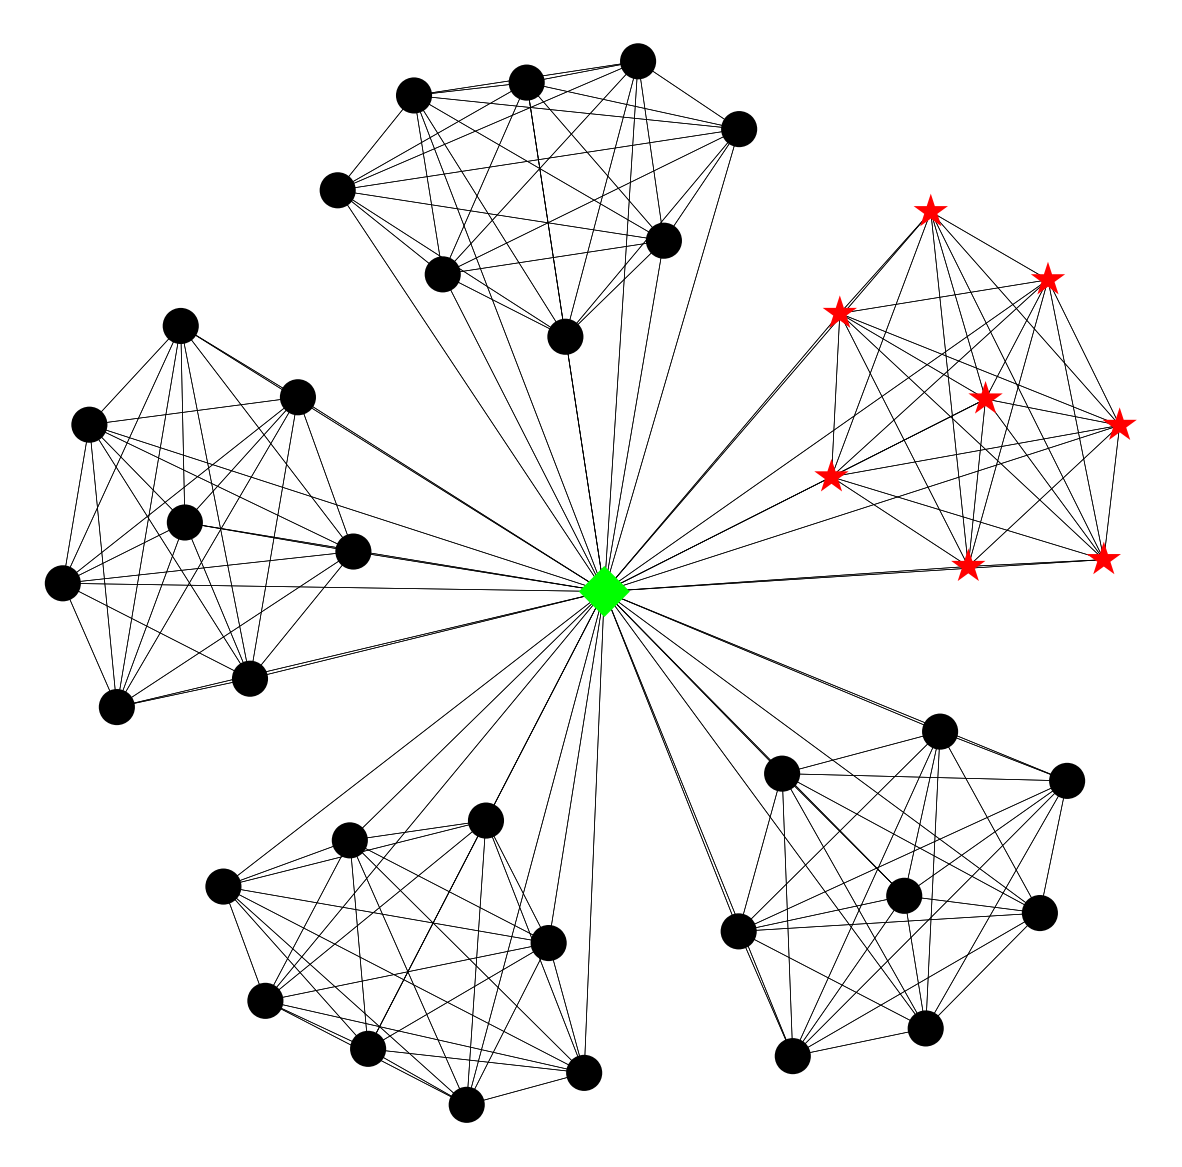
\includegraphics[width=0.3\linewidth]{media/From_ASONAM/Graphs/rep_soc_graph.png}\label{subfig:rep_soc_graph}}
    \hfill
    \subfloat[Ring of stars]{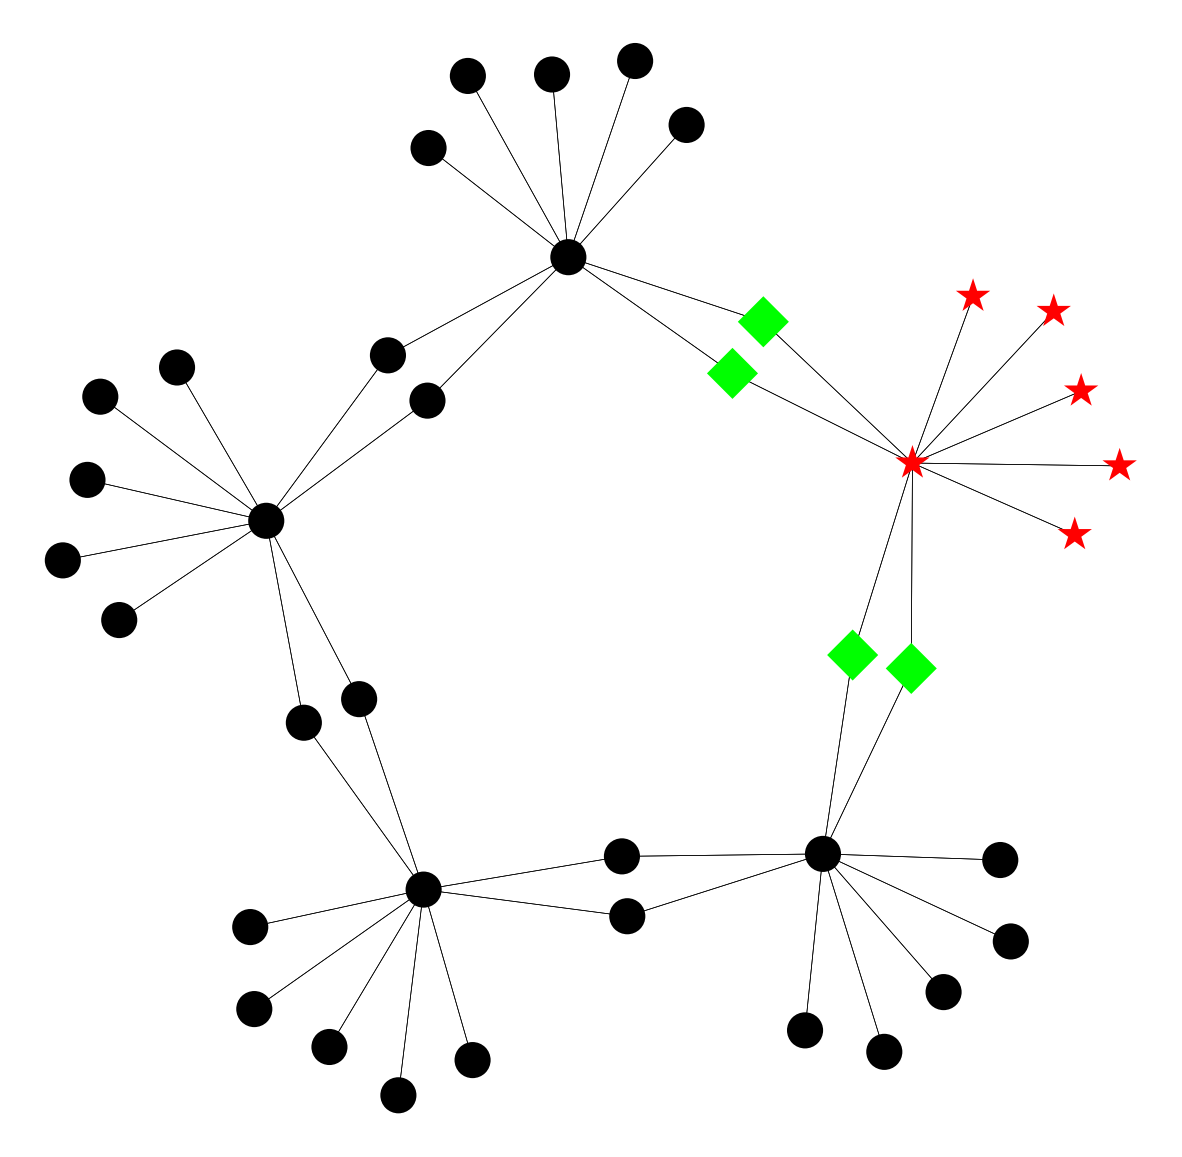
\includegraphics[width=0.3\linewidth]{media/From_ASONAM/Graphs/rep_ros_graph.png}\label{subfig:rep_ros_graph}}
    \hfill
    \subfloat[Toy Graph from SBM]{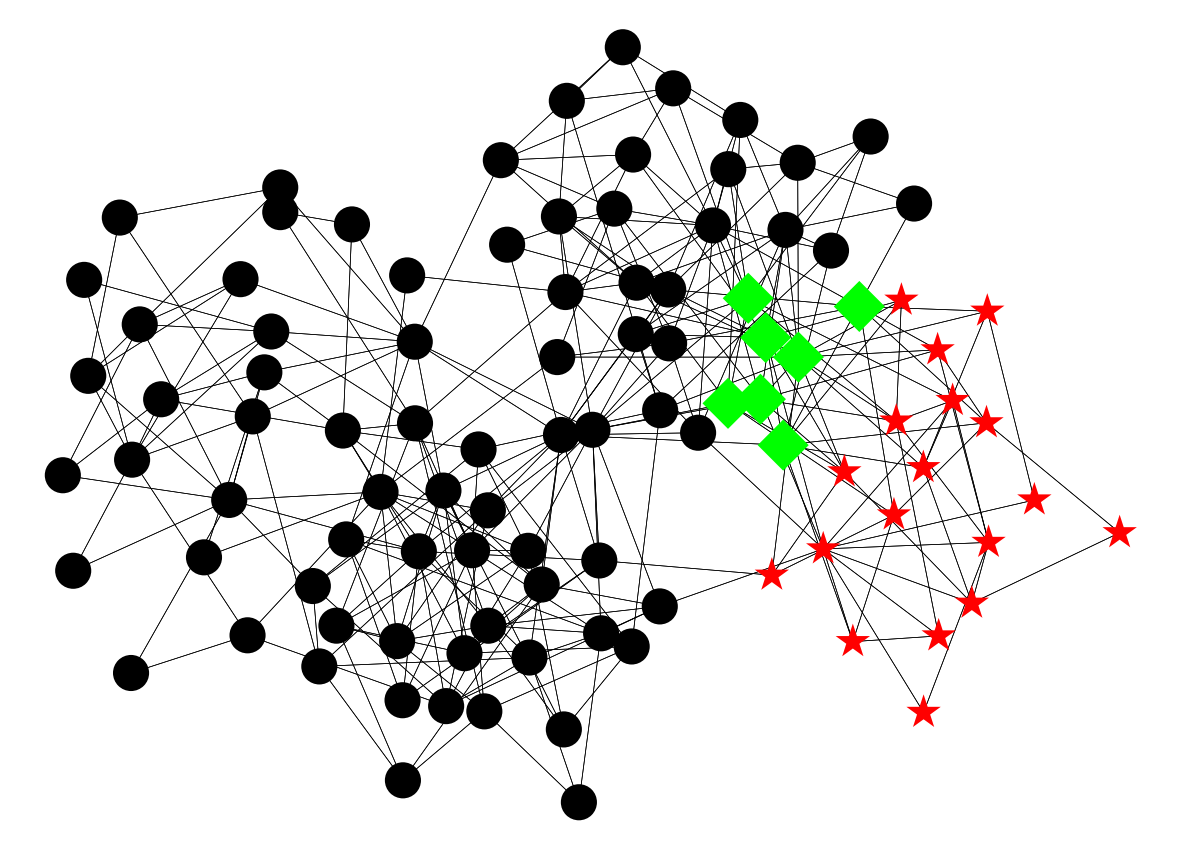
\includegraphics[width=0.3\linewidth]{media/From_ASONAM/Graphs/rep_toy_graph.png}\label{subfig:rep_toy_graph}}

    \subfloat[$\mat{\Pi} - \alpha \identity{n}$ matrix of the star of cliques]{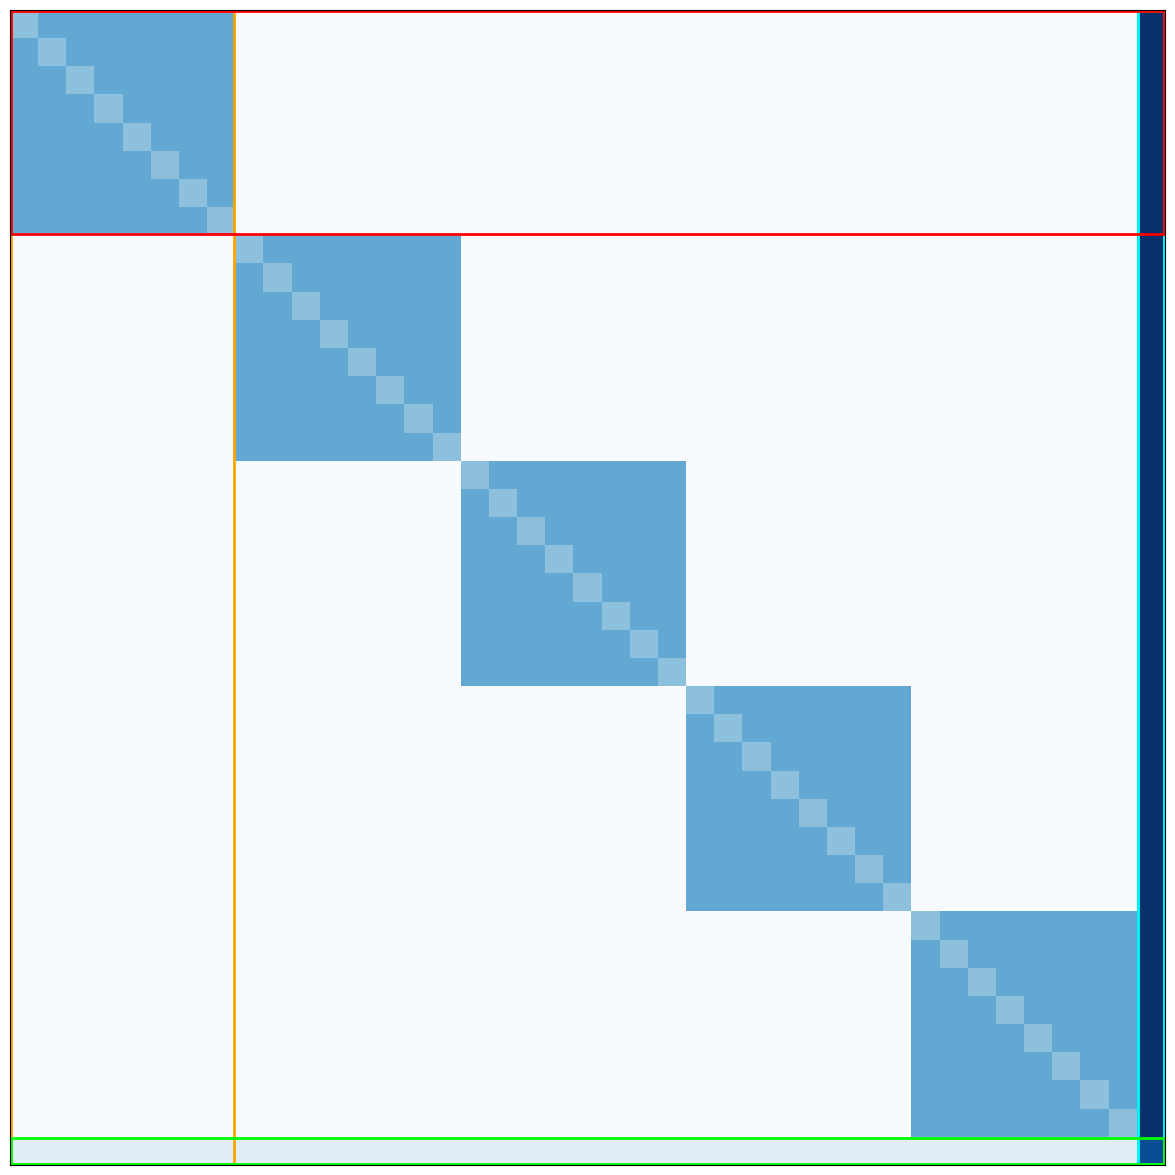
\includegraphics[width=0.3\linewidth]{media/From_ASONAM/PPR_matrices/ppr_mat_soc_graph.png}\label{subfig:ppr_mat_soc_graph}}
    \hfill
    \subfloat[$\mat{\Pi} - \alpha \identity{n}$ matrix of the ring of stars]{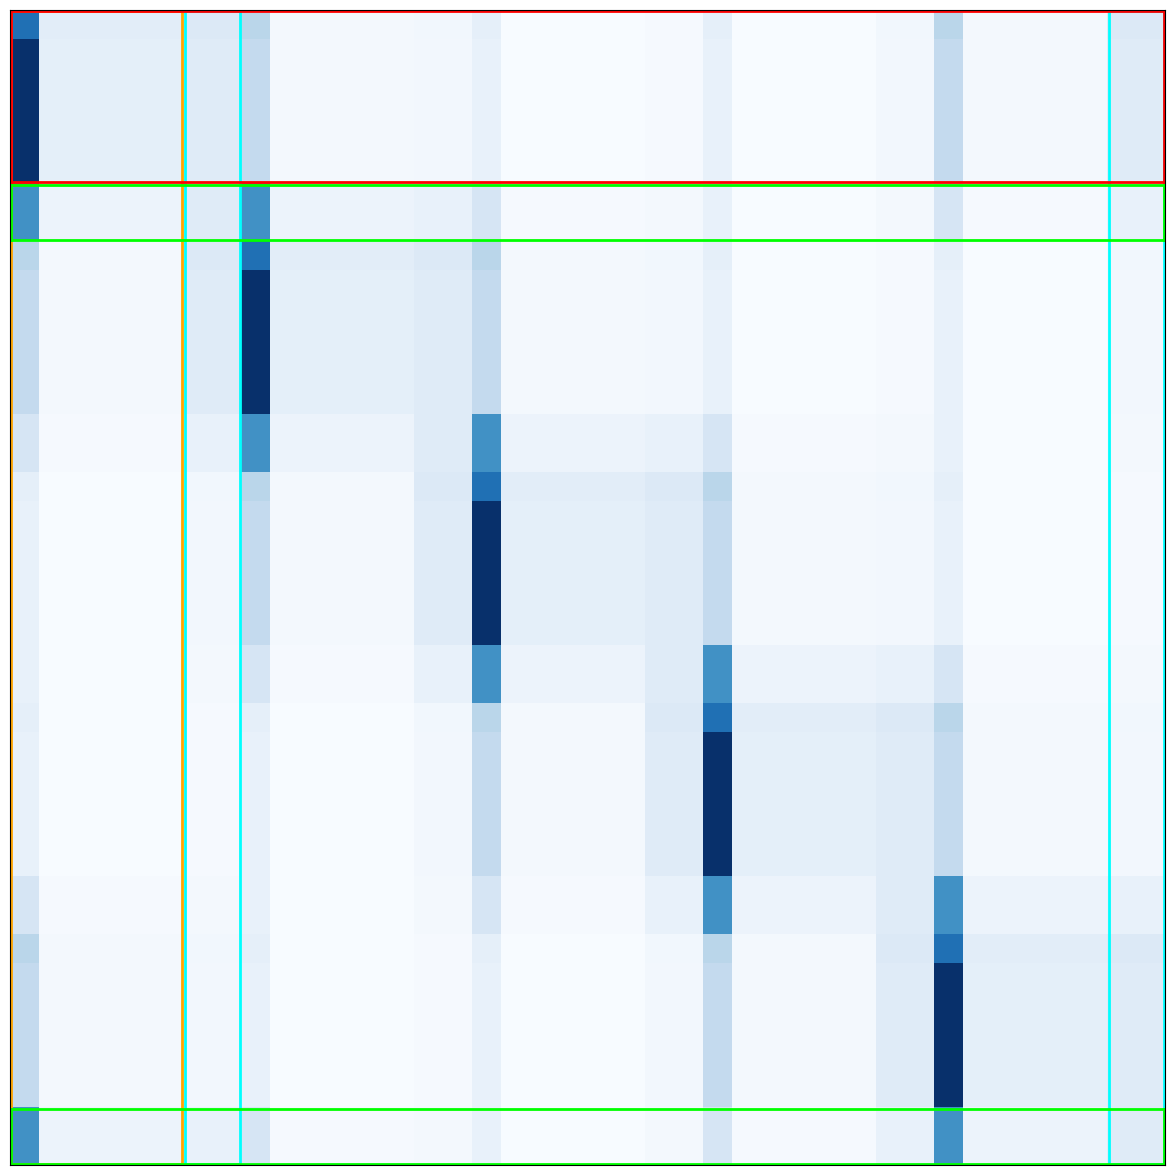
\includegraphics[width=0.3\linewidth]{media/From_ASONAM/PPR_matrices/ppr_mat_ros_graph.png}\label{subfig:ppr_mat_ros_graph}}
    \hfill
    \subfloat[$\mat{\Pi} - \alpha \identity{n}$ matrix of the toy graph from SBM]{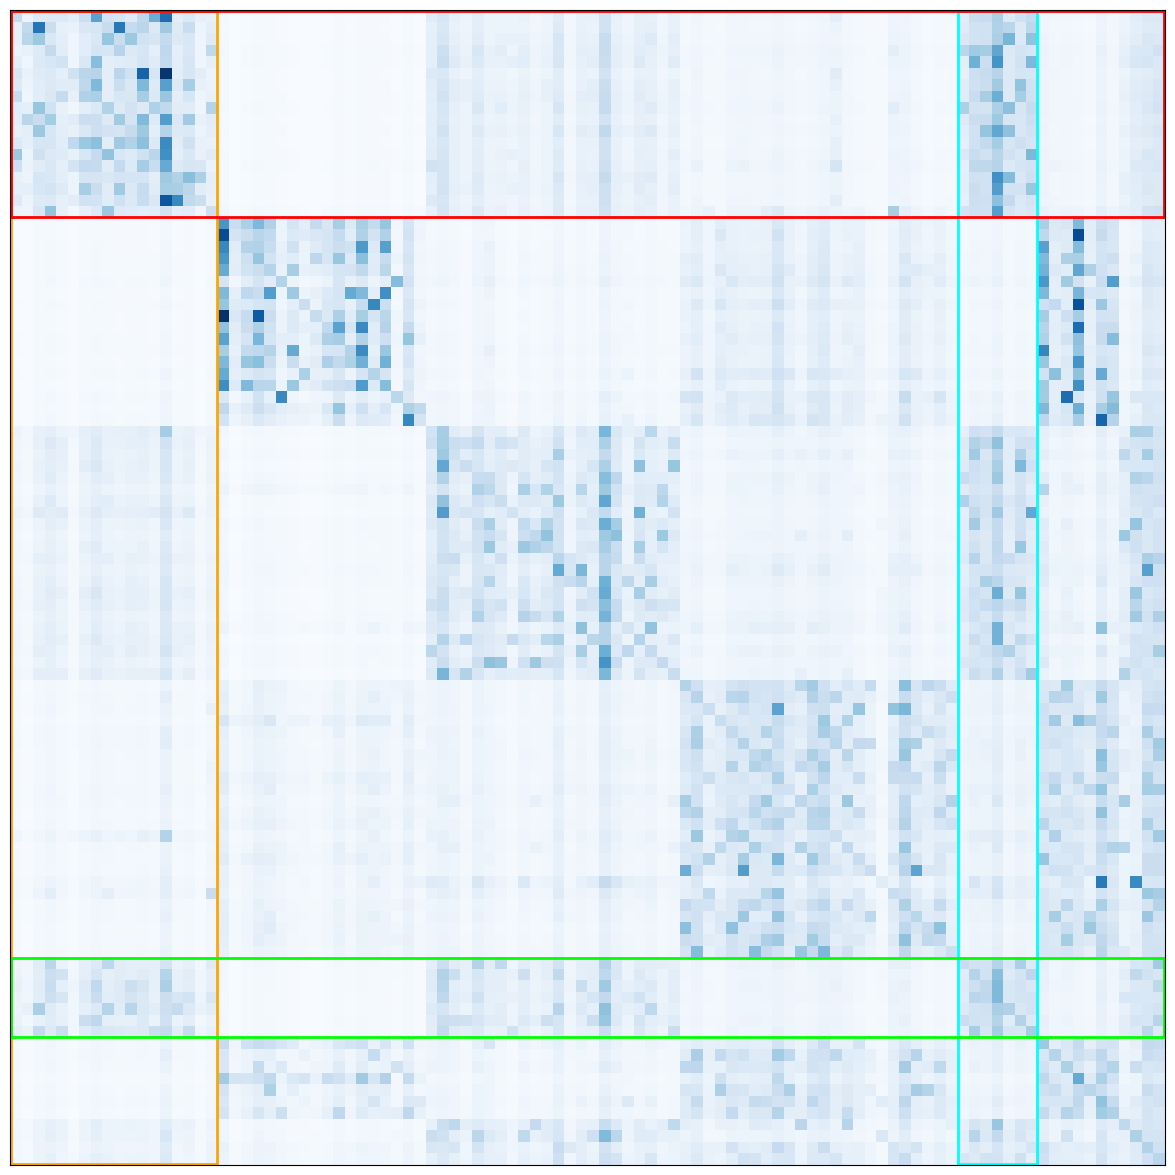
\includegraphics[width=0.3\linewidth]{media/From_ASONAM/PPR_matrices/ppr_mat_toy_graph.png}\label{subfig:ppr_mat_toy_graph}}
    %\subfloat[PPR matrix of the toy graph]{\includesvg[width=0.45\linewidth]{Figures/SBM_PPR.svg}\label{subfig:SBM_PPR}}
    \caption[Toy graphs and their respective $\mat{\Pi} - \alpha \identity{n}$ matrices]{Toy graphs and their respective $\mat{\Pi} - \alpha \identity{n}$ matrices. On each graph, a community is highlighted, the red stars vertices belonging exclusively to the community, and the green diamonds ones belonging both to the highlighted community and to at least one other. On each matrix, the rows and columns relative to the red star vertices are highlighted through red and orange boxes, and the rows and columns relative to the green diamond vertices are highlighted through green and cyan boxes.  We use $\mat{\Pi} - \alpha \identity{n}$ instead of $\mat{\Pi}$ for better readability.}
    \label{fig:graphs_PPR}
\end{figure*}

%One of the main advantages of the SVD, that make it especially attractive for embedding, is that it is known to filter out the noise in the data. More specifically, the SVD removes the small variations between data so that only the main patterns in the matrix are kept in the final result \cite{SVD_filtering_data}.
\todo{Use this paragraph in "our approach" part ?}

\subsection{Our approaches}\label{sec:approach}\todo{Approaches ? (plural ?)}
\subsubsection{Overview} \label{subsec:overview}
We introduce the new PAgeRank FActorization-based InTerpretable Embedding (\parfaite{}) method. It produces two embeddings, \newembLeft{} (left) and \newembRight{} (right).

Our method consists of three main parts. First, a truncated Singular Values Decomposition is performed on the centered PPR matrix. To overcome the issues of computing and representing the PPR matrix exactly for very large graphs, we employ a function $m$ that, given any vector $\vect{v}$, approximates the multiplication of the matrix with the vector. This results in two representations of the vertices as $\mat{U}\mat{\Sigma}$ and $\mat{V}\mat{\Sigma}$.

Then, vertices are clustered, with each vertex being represented by a concatenation of its left and right representation. This provides the central points of the communities in the space of these representations, stored in the matrix $\mat{C}$. Finally, our left and right embeddings, respectively \newembLeft{} and \newembRight{} are computed by projecting back these central points onto the original spaces. A pseudocode of our algorithm is shown in Algorithm~\ref{algo:emb}. 

\begin{algorithm}
    \caption{\parfaite{}}\label{algo:emb}
    \begin{algorithmic}[1]
    \Procedure{\parfaite{}}{$\mat{P}$: stochastic random walk matrix, $m_P$: function that approximate $\mat{\Bar{\Pi}}\vect{v}$ for any $\vect{v}$}
    %\KwResult{$\mat{C_l}, \mat{C_r}$ the left and right embeddings}
    \State $\mat{U}$, $\mat{\Sigma}$, $\mat{V}$ $\gets$ SVD($m_P$)
    \State clustering $\gets$ kmeans(concat( normalize($\mat{U}\mat{\Sigma}$), normalize($\mat{V}\mat{\Sigma}$)))
    \State $\mat{C} \gets$ clustering.clusters\_centers
    \State \newembLeft{} $ \gets \mat{U}\mat{C}_{\cdot, d:}^\top$
    \State\newembRight{} $ \gets \mat{V}\mat{C}_{\cdot, :d}^\top$
    \State \textbf{return} \newembLeft{}, \newembRight{}
    \EndProcedure
    \end{algorithmic}
\end{algorithm}

\subsubsection{Interpretation of the steps}\label{subsec:interpretation}


The \parfaite{} method relies on the well-established fact that the PPR vector of each vertex often contains large scores at dimensions corresponding to vertices it shares at least one community with, while it contains small scores at other dimensions \cite{Hollocou2017,Kloumann2014}. When we consider the PPR vector as a relevance scoring of the vertices of the graph wrt. the source vertex, it means that the vertices of the graph that are the most relevant to the source vertex are those which share a community with it.

This property strengthens the one stated by \cite{zhang_2020} that two nodes are likely to share a community not only if the PPR score from one node to the other is high, but especially if their PPR vectors are similar., meaning that they “agree with each other in terms of their personalized views about the network” \cite{zhang_2020}.


We illustrate this property with three toy graphs represented in Figure~\ref{fig:graphs_PPR}. The first two graphs provide ideal cases where we can find communities according to two natural community definitions: a) a clique, where each node is connected to every other node in the community,
and b) a star where all nodes but one are connected to a single node (e.g. they are connected to a same influencer in social media). In particular, Figure~\ref{subfig:rep_soc_graph} represents a star of cliques, while Figure~\ref{subfig:rep_ros_graph} represents a ring of stars. Observe that the communities in the graphs of Figure~\ref{fig:graphs_PPR} do \define{overlap}, which means that some nodes belong to several communities at the same time. On each graph represented in Figure~\ref{fig:graphs_PPR}, one community is outlined. Red star vertices are those that belong exclusively to the outlined community, while green diamond vertices belong to the outlined community and at least another one. The graph in Figure~\ref{subfig:rep_toy_graph} is built using the Stochastic Block Model (SBM) with 100 vertices, 300 edges, 4 communities, with each pair of vertices of a same community being $100$ times more likely to be connected than two vertices from different communities. As a result, in Figure~\ref{subfig:rep_toy_graph}, there are 19 vertices belonging to exactly two communities, 7 of which are depicted in green. 

Figures~\ref{subfig:ppr_mat_soc_graph}, \ref{subfig:ppr_mat_ros_graph} and~\ref{subfig:ppr_mat_toy_graph} show the corresponding PPR matrices. Recall that each row corresponds to some vertex $v$ and it represents the PPR vector of $v$, that is the PPR scores when $v$ is the source vertex of the random walk. Indeed, we can see that PPR vectors contain larger scores to vertices of a same community as the source node, generating “square” patterns in the matrices.

Similarly, we observe that the reversed PPR vectors (columns in the matrix) exhibit the same pattern of large scores inside the community and low scores outside.

However, there might be relatively few vertices that have very large PPR scores even if they do not share communities with other nodes. This is apparent in Figure~\ref{subfig:ppr_mat_ros_graph}, where we observe that the central nodes in the neighboring cliques have higher scores in the PPR vector of the studied community than other nodes in the same community. The reversed PPR is not affected by that issue.

To avoid this bias, we define the $\mat{\Bar{\Pi}}$ matrix obtained by centering the columns of $\mat{\Pi}$.\todo{Introduce the proba we are talking about}

\begin{property}
    \begin{equation*}
        \mat{\Bar{\Pi}}_{i, j} = \frac{1}{n}\proba{X_f = j}\big(\proba{X_0=i|X_f=j}-\proba{X_0 = i}\big)
    \end{equation*}
\end{property}

\begin{proof}
\begin{align*}
        \mat{\Bar{\Pi}}_{i, j} & =  \proba{X_f = j | X_0 = i} - \proba{X_f = j} \\
         & =  \frac{\proba{X_0 = i | X_f = j}\proba{X_f = j}}{
            \proba{X_0=i}
            %\underbrace{\proba{X_0=i}}_{1/n}
        }
         - \proba{X_f = j}
\end{align*}
\end{proof}

If we look at the rows of this new matrix, each entry is then the excess of probability to go to each vertex from the reference vertex, compared to the agnostic probability. If we look at the columns and because $\proba{X_f =j}$ is a constant along a column, each entry is proportional to the excess of probability to come from each vertex given that the walk arrived at the reference vertex.

Because the SVD only keeps the main patterns of the matrix it decomposes as we saw in section \todo{link section back svd}, we expect the result of the SVD to exhibit the typical rows and columns for each community, i.e. the patterns of the excess of probability to respectively come from and arrive into the community given that we respectively arrived into and came from the community.
We could then interpret these vectors as respectively the belonging of each node to the community and its relevance wrt. the community.

Our last problem is that, although the truncated SVD should make the community patterns in the matrix apparent, each dimension of the decomposition usually does not match a community, hindering the interpretation. To tackle this issue, we perform a clustering on the vertices represented by the SVD, and we use the central points to obtain the desired representative vectors for each community. Note that, although the clustering itself is non-overlapping and non-fuzzy, the resulting vectors are fuzzy scoring of belonging and importance of the nodes in each community.\todo{Illustrate on toy graph?}

\subsubsection{Decomposition of the PPR matrix}
The PPR matrix is a dense matrix belonging to $\realset^{n\times n}$. In most cases of big graphs, this matrix is too big to be explicitly represented. As we saw in section \todo{Ref to back SVD}, most modern SVD algorithms don't require an explicit representation of the matrix $\mat{M}$ but only a function $m(\vect{v}) = \mat{M}\vect{v}$. We use a reduced form of equation \eqref{eq:ppr_mat_as_series} to approximate the PPR matrix.

\begin{equation}
    m(\vect{v}) = \mat{\Bar{\Pi}_l}\vect{v} = (\alpha \sum_{i=0}^l (1-\alpha)^i\mat{P}^i\vect{v}) - (\vect{\pi} \cdot \vect{v}) \vect{1}
\end{equation}
\noindent where $\vect{1}$ is the vector of which all entries equal $1$ and $\vect{\pi}$ is the (not-personalized) PageRank vector of the matrix.

We know from \cite{Kloumann2014} that a few steps are usually enough to compute an approximation of the PageRank vector that outlines the community of the node. We fix $l=10$ for the rest of this section.

\subsubsection{Finding the communities}
SVD provides representations that should, if used to reconstruct the matrix, contain only the main patterns of the matrix which are the communities. There is no reason however to think that the dimensions of the representations correspond themselves to communities. That is why we perform a clustering of the vertices using their SVD representations to find the communities. Since both matrices of the embedding provide relevant and distinct information, there is no reason to exclude one and therefore we use a concatenation of both sides as the vectors for the clustering. 
Unfortunately, we did not have enough time during this thesis to study which clustering algorithm would perform best for this task, and we simply use the well-known k-means++ algorithm and its initialization variant k-means++.

As we saw before, the PPR and reversed PPR vectors for vertices of a same community are expected to have similar patterns of high and low entries, which correspond to similar directions of the vectors. They are however not supposed to have similar norms, especially for the reversed PPR, for which the norm typically follows the importance of the vertex. To make the clustering algorithm work on directions and not on Euclidean distance, both embeddings are normalized before concatenation and then the cosine similarity is used.

\subsubsection{Reconstructing the communities rows and columns}
The $\mat{U}\mat{\Sigma}$ and $\mat{V}\mat{\Sigma}$ embeddings are the projection of the columns and rows of the centered PPR matrix onto the singular spaces, e.g. for a vertex of the graph $w$, we have $ (\mat{U}\mat{\Sigma})_{w, \cdot} = \vect{\Bar{\pi}_w}^\top\mat{V}$. Therefore, the clusters centers are the central columns and rows of each community, projected on the singular spaces. To reconstruct the true central columns and rows of the communities, which are the typical centered reversed PPR and centered PPR vectors for the community, we multiply by the transposed of the projection matrices, which are $\mat{U}$ and $\mat{V}$. Note that this reconstruction is not perfect because the dimensions of the singular spaces we use are smaller than the dimension of the original space.
\todo{Look at Galerkin method that can justify this way of doing}

\subsection{Experiments}\label{sec:parfaite_exp}

Our main goal is to show that our method provides better interpretability scores than state-of-the-art approaches, while boasting similar results for a popular machine learning task in graph analysis, such as link prediction. 

\noindent\textbf{Datasets.}
We use two datasets that are available on the SNAP website \cite{SNAP_paper}. The first one named \textit{Wikispeedia} contains 4592 vertices, and 120~000 edges. 105 overlapping ground-truth community are given. The second one named \textit{Facebook} contains 10 graphs. We exclude 2 of them, numbered 698 and 3980, because they contain less than 128 nodes and we could therefore not compute the SVD for them using the same parameters used for the others. The remaining 8 graphs contain between 155 and 1035 vertices and between 3312 and 60050 edges. Between 7 and 46 overlapping ground-truth communities are given for each graph.

We also use our new WikipediaFr dataset that contains 2.52 millions vertices, 102 million edges and 2~700 ground-truth communities. To keep the dimension of the embeddings manageable however, we only study the 117 communities that contain more than 10~000 vertices.

%We also release a new dataset with ground-truth communities\footnote{https://gitlab.telecom-paris.fr/gabriel.damay/WikipediaFRNetwork} (Wikipedia fr), constructed from all the pages of the French version of Wikipedia.\footnote{All the pages from the main space of Wikipedia, that is all the pages usually accessed by public, excluding discussions, user pages etc.} In such a graph, nodes represent Wikipedia pages while directed edges represent links between the corresponding Wikipedia pages. In the French version of Wikipedia, it is common to add links to so called ``portals'' at the end of the page which serve as reference pages for given topics and can be seen as ground-truth communities. %We observe that links to portals are more rare in the English version of Wikipedia, while portals are more semantically related to their corresponding Wikipedia pages than Wikipedia categories.
%Such novel graph contains 2.52 millions vertices, 102 million edges and 2~700 ground-truth communities. 
\todo{Make a section for WikipediaFr}

\noindent\textbf{Methods.} 
We evaluate our method against the two widely used algorithms for graph embedding HOPE and node2vec described in section \ref{subsec:embedding_history}.

We evaluate all methods in terms of the IS, BCI, CCI and CISIP metrics, discussed in section \ref{subsec:interpretability_explained}. However, we consider the BCI and CCI results with a skepticism\todo{Check if results are good, and if they are say it.} because of the limitations due to their normalization, as explained in the aforementioned section.
We include in our experiments embeddings produced by the state-of-the-art node2vec and HOPE algorithms and our 2 new embeddings \newembLeft{} and \newembRight{}.

For node2vec, we use the most-used python3 implementation \cite{node2vec_impl}. We keep the default parameters, i.e. the number of walks is 200 per vertex, the length of the walks is 30 and the window size is 10.

For HOPE, we use the official implementation in Matlab\footnote{https://github.com/ZW-ZHANG/HOPE} provided by the authors of \cite{HOPE} that we reimplement in python3 (while using numpy and scipy), to provide a fair comparison with the other approaches. We keep all the constants and parameters as available in this implementation.
%\todo{Make the implementation available}

Our algorithm is implemented in python3, using mainly the numpy \cite{numpy} and scipy \cite{scipy} packages. The jump parameter $\alpha$ for the PPR algorithm is set to $\alpha=0.1$. The number $l$ of iterations to approximate the PPR matrix is set to $l=10$ and the dimension $D$ of the intermediate SVD is set to $D=128$.\todo{Rename dimension? $D$ is supposed to be the diagonal matrix}

For all embeddings, %and in order to optimize the potential interpretability,
the dimension $K$ of the embedding is set to be the number $G$ of known ground-truth communities.

\noindent\textbf{Metrics.} We measure the interpretability of the methods using each of the metrics mentioned in the “metrics” part of the section \ref{subsec:interpretability_explained}. The Interpretability Scores (IS) are aggregated along the ground-truth groups using the max function, and then along the embedding dimensions using the sum function.
The size of the top and bottom sets considered for the Betweenness and Closeness Centrality Indices (BCI and CCI) are set to the size of the studied ground-truth group, as suggested by the original paper.
For CISIP, three smoothing functions $f$ are considered. The first one, that we call “identity” is the direct use of the binary belonging feature, the second one is the Mean Neighbors Belonging (MNB), that is the mean of the belonging features of the neighbors, and the last one is the PPR of the community.

The BCI and CCI are not computed for the WikipediaFr for performances reasons.

\subsection{Results}
The results are given in Table~\ref{tab:IS_scores} \todo{Add all results}and~\ref{tab:CISIP_scores}. Because of space limitation, only Facebook 107 and 1912, as parts with the highest degree and order of Facebook, are presented, as well as Facebook 3437 because of the good performances of HOPE on this dataset with the CISIP-identity metric. The results for the other versions of Facebook are similar to what is presented.

As we see in these results, our algorithm's interpretability is much higher than node2vec's when evaluated using the Interpretability Score or any of the variants of CISIP. HOPE's interpretability is closer, but still generally below \parfaite{}'s.

Our left embedding greatly outperforms the right one when using CISIP with the PPR smoothing, and this result was expected, as the left embedding is an approximation of the typical PPR vector of each cluster detected. The results are however equivalent between our two embeddings when compared using either the IS or CISIP with the identity smoothing, which both evaluate directly the matching between the embedding and the belonging features, or with the MNB smoothing. This is consistent with our interpretation that the left embedding represents which communities a vertex belongs to, while the right embedding measures somehow the “importance” of a vertex in a community.

\subsection{Is the clustering needed ?}
To check if the last step of our algorithm of clustering the data and computing the final embeddings is really needed, we compare our results to what we would have without the clustering step. To achieve this, we take the $\mat{U}\mat{\Sigma}$ and $\mat{V}\mat{\Sigma}$ results from the SVD, and we keep only the $G$ first dimensions to match the dimension of the \parfaite{} embeddings so that the dimension of this embedding is identical to the dimension of the \parfaite{} embeddings.

The results for IS and for CISIP with the three smoothing functions already used are presented in Table~\ref{tab:IS_SVD_scores} and~\ref{tab:CISIP_SVD_scores}. We see that in most cases the results of our \newembLeft{} and \newembRight{} outperform those before clustering, sometimes significantly (e.g. more than $0.1$ points of difference for the IS). This is especially true for the IS and CISIP with PPR smoothing. We note however that the SVD provides better results in several occurrences when compared to our embeddings using CISIP with the identity or the MNB smoothing.

Overall we conclude that \newembLeft{} and \newembRight{} do generally perform better than single SVD, i.e. without the clustering and reconstruction steps.

\subsection{Is our embedding efficient ?}
The method we propose mainly focuses on the interpretability of the embedding. This interpretability should however not come at the cost of an excessive loss of efficiency in the task the embedding helps to solve.

We check the efficiency of \parfaite{} against HOPE and node2vec at the task of Link Prediction. We build test graphs by removing 0.1\% of the edges of a real-world graph. We store the pairs of vertices of these edges as “positive” pairs, and build a set of “negative” pairs by drawing the same number of pairs of vertices that are not connected by an edge.

The embedding of the test graph is computed, and a score is attributed to each positive or negative pair of vertices using this embedding.

For HOPE, the score is the dot product of the left embedding of the first vertex in the pair and the right embedding of the second vertex. The score for \parfaite{} is similar, but the left embedding of the first vertex is normalized to account for the entire use of the singular values on each side of the embedding. For node2vec, following \cite{groverNode2vecScalableFeature2016}, a Logistic Regression is trained on the test graph by representing the pairs with a concatenation of their vertices' embeddings.

We run this experiment on 10 test graph for both the Wikispeedia dataset and on the 1912 part of the Facebook dataset, as the part with the highest order. The mean results are given in Figure \ref{fig:lp_results}. As we can see, node2vec is outperformed by both HOPE and \parfaite{}. HOPE achieves similar results as \parfaite{} on Facebook~1912 and slightly better on Wikispeedia, but overall we can say that the greater interpretability of \parfaite{} does not come at the cost of lower efficiency on the task of link prediction.

\begin{figure}
   \centering
    \subfloat[Wikispeedia]{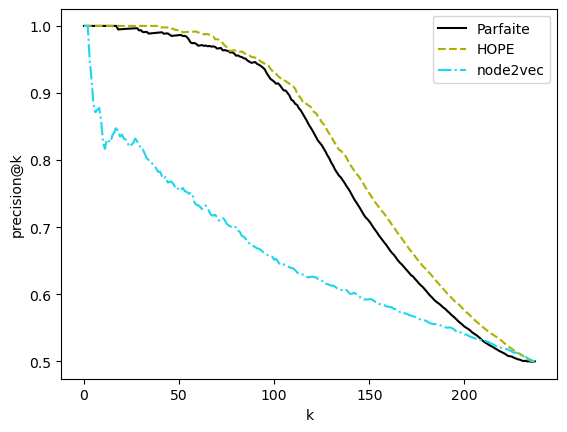
\includegraphics[width=0.5\linewidth]{media/From_ASONAM/LP/LP_results_wikispeedia.png}\label{subfig:lp_wikispeedia}}
    \subfloat[Facebook 1912]{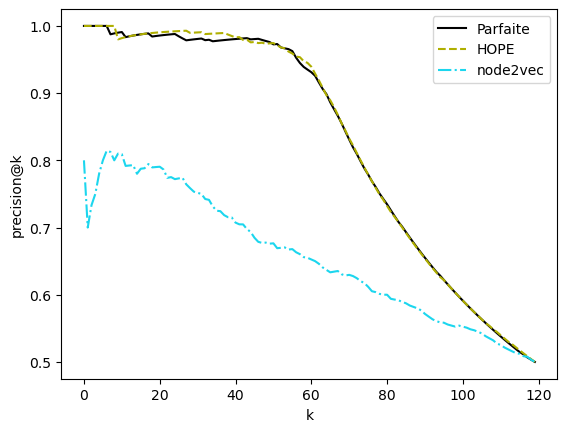
\includegraphics[width=0.5\linewidth]{media/From_ASONAM/LP/LP_results_facebook.png}\label{subfig:lp_facebook}}
    \caption[Precision@k results of the Link Prediction experiment]{Mean Precision@k of the Link Prediction on 20 test graphs built from the Wikispeedia and Facebook 1912 datasets}
    \label{fig:lp_results}
\end{figure}

\section{Conclusion and future work}\label{sec:conclusion}
We have presented \parfaite{}, a novel graph embedding algorithm and we have evaluated its interpretability against the state-of-the-art node2vec and HOPE algorithms. We also presented the new interpretability score CISIP to assure that interpretations are well-separated and non-redundant.
Our approach relies on the clustering of the vertex embeddings, for which we use the $k$-means algorithm. An interesting direction for future work would be to study whether other clustering methods provide better results. We have also seen that, although the clustering phase increases the interpretability of our embedding, in some rare cases clustering might have a negative impact on the interpretability. It would be interesting to have a better understanding of this phenomenon, which could pave the way for a more effective approach.  Finally, the CISIP metric contains a smoothing function as a parameter and it would be interesting to study the properties of various functions for this task and what they imply in terms of interpretability of the embedding at hand.

\begin{table}[t]
    \caption{Interpretability Score results for \parfaite{}, HOPE and node2vec}
    \begin{center}
        \begin{tabular}{l|c|c|c|c|c}
            \hline
            \textbf{Dataset} & \multicolumn{2}{|c|}{\textbf{\parfaite{}}} & \multicolumn{2}{|c|}{\textbf{HOPE}} & \textbf{node2vec}\\
            & left & right & left & right\\
            \hline
Wikispeedia  &  \textbf{0.389} & 0.375 & 0.200 & 0.266 & 0.139\\
%\hline
Facebook 0 & 0.520 & \textbf{0.567} & 0.529 & 0.530 & 0.429\\
%\hline
Facebook 107 & \textbf{0.626} & 0.601 & 0.550 & 0.550 & 0.323\\
%\hline
Facebook 348 & \textbf{0.968} & 0.928 & 0.888 & 0.888 & 0.895\\
%\hline
Facebook 414 & 0.854 & \textbf{0.861} & 0.683 & 0.683 & 0.414\\
%\hline
Facebook 686 & \textbf{0.736} & 0.730 & 0.650 & 0.650 & 0.617\\
%\hline
Facebook 1684 & \textbf{0.863} & 0.807 & 0.572 & 0.572 & 0.304\\
%\hline
Facebook 1912 & \textbf{0.766} & 0.764 & 0.603 & 0.603 & 0.348\\
%\hline
Facebook 3437 & 0.430 & \textbf{0.759} & 0.429 & 0.429 & 0.188\\
%\hline
WikipediaFr  &  0.040 & \textbf{0.083} & 0.041 & \textbf{0.083} & *\\
\hline
        \end{tabular}
    \end{center}
    \label{tab:IS_scores}
    * The embedding of this graph with node2vec as been stopped after 36h of computation.
\end{table}



\begin{table}[t]
\caption{CISIP results for \parfaite{}, HOPE and node2vec}
\begin{center}
\begin{tabular}{l|c|c|c|c|c}
\hline
%\textbf{Dataset} & \textbf{\newembLeft{}} & \textbf{\newembRight{}} & \textbf{node2vec} & \textbf{HOPE (l)} & \textbf{HOPE (r)}\\
\textbf{Dataset} & \multicolumn{2}{|c|}{\textbf{\parfaite{}}} & \multicolumn{2}{|c|}{\textbf{HOPE}} & \textbf{node2vec}\\
& left & right & left & right\\
\hline
\multicolumn{6}{c}{No smoothing (identity function)}\\
\hline
Wikispeedia  &  \textbf{0.429} & 0.414 & 0.339 & 0.318 & 0.255 \\
%\hline
Facebook 0 & \textbf{0.333} & 0.311 & 0.233 & 0.232 & 0.248 \\
%\hline
Facebook 107 & 0.403 & \textbf{0.408} & 0.316 & 0.316 & 0.234 \\
%\hline
Facebook 348 & 0.561 & \textbf{0.566} & 0.524 & 0.524 & 0.252\\
%\hline
Facebook 414 & 0.545 & \textbf{0.605} & 0.540 & 0.540 & 0.283\\
%\hline
Facebook 686 & \textbf{0.527} & 0.489 & 0.384 & 0.384 & 0.295\\
%\hline
Facebook 1684 & 0.483 & \textbf{0.493} & 0.369 & 0.369 & 0.264  \\
%\hline
Facebook 1912 & 0.401 & \textbf{0.425} & 0.352 & 0.353 & 0.266\\
%\hline
Facebook 3437 & 0.300 & 0.310 & \textbf{0.331} & \textbf{0.331} & 0.256\\
%\hline
WikipediaFr  &  0.350 & \textbf{0.376} & 0.339 & 0.353 & *\\
\hline
\multicolumn{6}{c}{Smoothing with MNB}\\
\hline
Wikispeedia  &  0.431 & \textbf{0.508} & 0.282 & 0.369 & 0.105 \\
%\hline
Facebook 0 & \textbf{0.436} & 0.434 & 0.230 & 0.230 & 0.028 \\
%\hline
Facebook 107 & \textbf{0.545} & 0.515 & 0.384 & 0.384 & 0.161\\
%\hline
Facebook 348 & \textbf{0.582} & 0.509 & 0.349 & 0.349 & 0.105\\
%\hline
Facebook 414 & \textbf{0.627} & 0.584 & 0.474 & 0.474 & 0.084\\
%\hline
Facebook 686 & \textbf{0.475} & 0.400 & 0.234 & 0.234 & 0.102\\
%\hline
Facebook 1684 & \textbf{0.539} & 0.532 & 0.389 & 0.389 & 0.122\\
%\hline
Facebook 1912 & 0.504 & \textbf{0.511} & 0.269 & 0.267 & 0.029\\
%\hline
Facebook 3437 & 0.513 & \textbf{0.524} & 0.373 & 0.373 & 0.067\\
%\hline
WikipediaFr  &  0.272 & \textbf{0.499} & 0.400 & 0.493 & *\\
\hline
\multicolumn{6}{c}{Smoothing with PPR}\\
\hline
Wikispeedia  &  0.449 & \textbf{0.516} & 0.189 & 0.174 & 0.012\\
%\hline
Facebook 0 & \textbf{0.429} & \textbf{0.429} & 0.143 & 0.138 & 0.074 \\
%\hline
Facebook 107 & \textbf{0.585} & 0.576 & 0.304 & 0.304 & 0.093 \\
%\hline
Facebook 348 & 0.633 & \textbf{0.682} & 0.510 & 0.510 & 0.071\\
%\hline
Facebook 414 & 0.589 & \textbf{0.774} & 0.531 & 0.531 & 0.283\\
%\hline
Facebook 686 & 0.454 & \textbf{0.550} & 0.285 & 0.285 & 0.106\\
%\hline
Facebook 1684 & 0.538 & \textbf{0.649} & 0.393 & 0.393 & 0.085 \\
%\hline
Facebook 1912 & 0.557 & \textbf{0.633} & 0.278 & 0.279 & 0.101\\
%\hline
Facebook 3437 & 0.568 & \textbf{0.688} & 0.402 & 0.402 & 0.073\\
%\hline
WikipediaFr  &  \textbf{0.123} & -0.067 & 0.049 & -0.015 & *\\
\hline
        \end{tabular}
    \end{center}
    \label{tab:CISIP_scores}
\end{table}

\begin{table}[t]
    \caption[Interpretability Score results for the SVD of the PPR matrix]{Interpretability Score results for the SVD of the PPR matrix. The results in bold as those at least as good as the related \parfaite{} results}
    \begin{center}
        \begin{tabular}{l|c|c}
            \hline
            \textbf{Dataset} & \textbf{SVD (left)} & \textbf{SVD (right)}\\
            \hline
Wikispeedia  & 0.234 & 0.204\\
%\hline
Facebook 0 & \textbf{0.538} & \textbf{0.593}\\
%\hline
Facebook 107 & 0.538 & 0.516\\
%\hline
Facebook 348 & 0.923 & \textbf{0.928}\\
%\hline
Facebook 414 & 0.808 & 0.812\\
%\hline
Facebook 686 & 0.690 & 0.696\\
%\hline
Facebook 1684 & 0.792 & 0.768\\
%\hline
Facebook 1912 & 0.589 & 0.604\\
%\hline
Facebook 3437 & 0.270 & 0.463\\
%\hline
WikipediaFr  & \textbf{0.043} & 0.061\\
\hline
        \end{tabular}
    \end{center}
    \label{tab:IS_SVD_scores}
\end{table}

\begin{table}[t]
\caption[CISIP results for the SVD of the PPR matrix]{CISIP results for the SVD of the PPR matrix. The results in bold as those at least as good as the related \parfaite{} results}
\begin{center}
\begin{tabular}{l|c|c}
\hline
\textbf{Dataset} & \textbf{SVD (left)} & \textbf{SVD (right)}\\
\hline
\multicolumn{3}{c}{No smoothing (identity function)}\\
\hline
Wikispeedia  & 0.363 & 0.362\\
%\hline
Facebook 0 & 0.333 & \textbf{0.360}\\
%\hline
Facebook 107 & \textbf{0.493} & \textbf{0.464}\\
%\hline
Facebook 348 & 0.520 & 0.525\\
%\hline
Facebook 414 & \textbf{0.545} & 0.549\\
%\hline
Facebook 686 & 0.438 & 0.440\\
%\hline
Facebook 1684 & \textbf{0.532} & \textbf{0.545}\\
%\hline
Facebook 1912 & 0.377 & 0.392\\
%\hline
Facebook 3437 & \textbf{0.304} & \textbf{0.337}\\
%\hline
WikipediaFr  & \textbf{0.350} & \textbf{0.381}\\
\hline
\multicolumn{3}{c}{Smoothing with MNB}\\
\hline
Wikispeedia  & 0.280 & 0.369\\
%\hline
Facebook 0 & 0.330 & 0.395\\
%\hline
Facebook 107 & \textbf{0.596} & \textbf{0.571}\\
%\hline
Facebook 348 & 0.404 & 0.412\\
%\hline
Facebook 414 & 0.431 & 0.404\\
%\hline
Facebook 686 & 0.320 & 0.337\\
%\hline
Facebook 1684 & 0.512 & 0.493\\
%\hline
Facebook 1912 & 0.299 & 0.320\\
%\hline
Facebook 3437 & 0.429 & 0.443\\
%\hline
WikipediaFr  & 0.259 & \textbf{0.502}\\
\hline
\multicolumn{3}{c}{Smoothing with PPR}\\
\hline
Wikispeedia  & 0.244 & 0.202\\
%\hline
Facebook 0 & 0.284 & 0.356\\
%\hline
Facebook 107 & \textbf{0.609} & \textbf{0.604}\\
%\hline
Facebook 348 & 0.449 & 0.485\\
%\hline
Facebook 414 & 0.527 & 0.541\\
%\hline
Facebook 686 & 0.378 & 0.407\\
%\hline
Facebook 1684 & 0.511 & 0.549\\
%\hline
Facebook 1912 & 0.319 & 0.320\\
%\hline
Facebook 3437 & 0.419 & 0.421\\
%\hline
WikipediaFr  & \textbf{0.150} & \textbf{-0.011}\\
\hline
\end{tabular}
\end{center}
\label{tab:CISIP_SVD_scores}
\end{table}

\section{A practical application: Detecting communities on a YouTube graph}
We teamed up with a company specialized in YouTube economics and data to extract a bipartite graph of YouTube. A \define{bipartite graph} is a graph in which the nodes are split into two parts and a node from one part can only share an edge with nodes of the other part. Each part usually represent a type of real-world entity. For example, here, one part represents the YouTube users while the other part represented YouTube videos. An edge represented the fact that the user had commented the video and it was weighted by the number of comments. However, due to technical limitations, we only had the last 15~000 comments on the videos of a same YouTube channel at the time of the scrapping.

The goal was to separate the graph into \define{clusters}, i.e. groups of nodes densely connected to one another, and sparsely connected to the rest of the graph. The graph had many small connected components and also some series of users connected to only a few videos, themselves connected to a few users. To remove these less interesting parts that made the clustering more difficult, we kept only the \define{$k$-core} of the graph, i.e. the maximal subgraph in which every node have at least $k$ neighbors. The values of $k$ we have considered $2$, $5$ and $10$. 

Then we tried two clustering methods in the graph. The first one computed a spectral embedding and then performed a k-means clustering on the resulting embedding. The second one used the Louvain algorithm, which is a well-known graph clustering algorithm, to cluster the data.

We presented the results as a small and easy website to help reading and browsing them\todo{Add screenshot}.

Unfortunately, the manual analysis of the results revealed poor performances. We worked with researchers interested in sociology who had partially clustered the videos and who did not find a convincing matching between their work and the results. After analyzing the data, we think that the limitation to the last 15~000 comments on the videos of a same YouTube channel removed a lot of information. For example, we probably lost a lot of the occurrences when a same user who was very loyal to a channel had commented on most of the videos at the time of their publication, because those comments would have been old and therefore “erased” by new comments.

\printbibliography

\todo{Check consistent use of "s" or "z" for "zation" words (e.g. "Minimization")}
\todo{Check footnotes after punctuation (except when refering to a specific word)}
\todo{Explicit and ensure consistency of use of "prediction" or "decision" for the output of classification algorithms}
\todo{Ensure consistency: "split condition"? "split criterion" => explicit that "condition" is used for binary trees}
\todo{Explicit tree building = tree training}
\todo{Unify a rule for indent (in latex: empty line) after Theorems-like environments}
\todo{Indicate that all non-transposed vectors are column?}
\todo{Clarify notations}
\todo{Check "symmetrical" $\rightarrow$ "symmetric"}
\todo{Check "they are" $\rightarrow$ "there are"}
\todo{Add Acknowledgements to ANR funding}
\todo{Unify "Parfaite" syntax (\textsc{PaRFaItE} ? )}
\todo{All matrices and vectors should use the \\mat and \\vect commands}
\todo{All probabilities should use the \\proba environment}
\todo{Identity matrices should use the dedicated command}
\todo{For old ref of the article, check that the ref is as good, or complete}
\todo{Check that we put the complete array of results, not the partial ones}
\todo{Check consistancy of BCI/CCI results promised and shown}
\todo{Check that odd-numbered pages are on the right (i.e. the last roman numbering is even or there is a blank page}
\todo{Check consistant use of the \\define environment}
\diplayLastPage
\end{document}